\chapter{Search for Non-resonant Signatures and Contact Interactions}\label{sec:ci}

% Physical processes that produce a pair of final state leptons offer a clear window into the dynamics of high energy collisions.
Observations of pairs of leptons, both of electron and muon flavors, offer a clear window into the dynamics of high energy collisions.
The clarity of this window is due to the long lifetime and ease of detection offered by those leptons.
Of particular use is the invariant-mass spectra of dilepton pairs, which elucidates the possible mechanisms of their production by means of local enhancements, or resonances. 
This has proved a useful tool that has been exploited throughout the history of experimental particle physics.
In 1974, a group working at Brookhaven National Laboratory\cite{jpsiBnl} and another group working at the Stanford Linear Accelerator Center\cite{jpsiSlac} used the dielectron mass spectrum to independently discover the \jpsi resonance at \mee=3.1~GeV.
In 1977, a group working at Fermilab used the dimuon mass spectrum to discover the $\Upsilon$ resonance at \muu=9.5~GeV \cite{upsilon}.
In 1983, the UA1 group working at the SPS collider at CERN used both dielectron and dimuon events to detect the decay of the \Z boson at a mass of $\mll\approx95$~GeV\cite{z0ua1}.
Later in the same year, the UA2 group used dielectron events to produce a measurement of \mee=91.9~GeV.
The utility of the dilepton final state is derived from the fact that the final state consisting of two leptons is fully reconstructible.

\begin{figure}[htp]
\captionsetup[subfigure]{position=b}
\centering
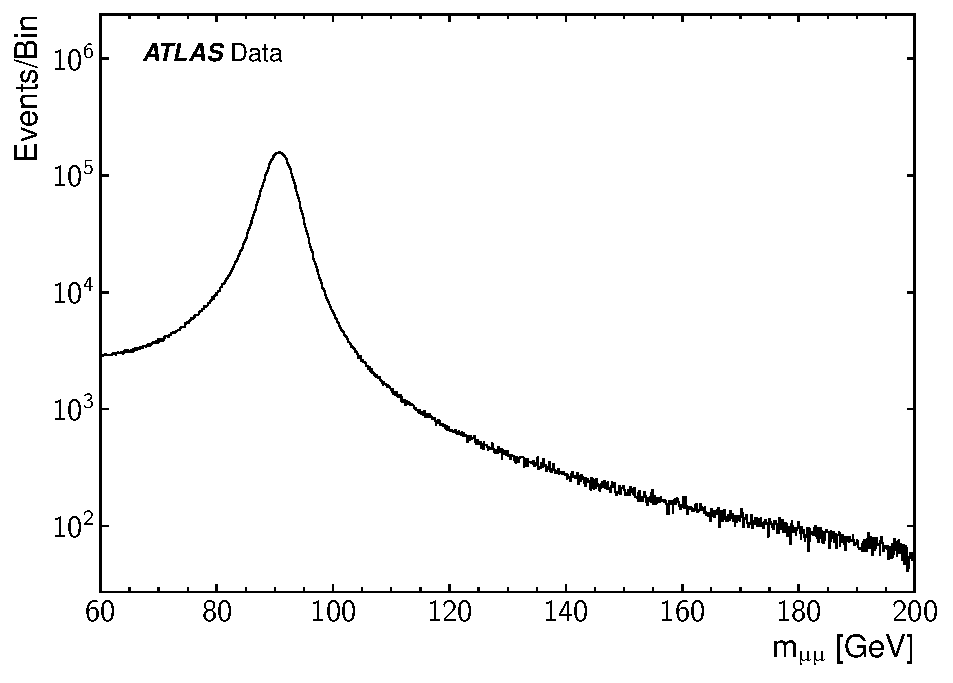
\includegraphics[width=0.7\textwidth]{figures/ci/lowmass/lowmass-lower.pdf}
\caption{The invariant-mass spectra around the \Z boson mass peak from one million collisions with two muons.}
\label{fig:ciLowMass}
\end{figure}

% General non-resonant
The discoveries made with the invariant-mass spectra associate enhancement in rate of observed events with new mechanisms responsible for the enhancement.
These enhancements may be localized, as is the case for narrow resonances produced by \jpsi decay.
Alternatively, broad enhancements are possible as well; such enhancements, termed \emph{non-resonant}, are the focus of this search.
\footnote{Broad deficits are possible as well; one example is the observations of negative (positive) interference between $\gamma^*$ and \Z that changes the forward-backward charge symmetry below (above) the \Z mass peak in electron-positron experiments \cite{fbasym}.}
The investigation presented in this chapter contemplates the dielectron and dimuon invariant mass spectra in search for new and broad excesses appearing in the high mass tail.

Many new physics models beyond the Standard Model predict broad enhancements in dilepton production.
% Contact interactions
A particularly interesting cause of a non-resonant signature is a \emph{contact interaction} (CI) between quarks and leptons at an energy scale exceeding that of the collision energy.
Although direct resonant production is inaccessible, a new contact interaction would lead to off-shell production and interference with the SM production.
This can be caused by a mediator particle with a mass far above the \sqrts=13~TeV collision energies offered by the LHC.
A \qqll CI is also interesting because it is a necessary outcome of quarks and leptons sharing a common substructure \cite{eichten}.

Many new physics models outside the Standard Model predict non-resonant excesses.
To maintain a degree of generality and model independence, the products of this search are designed to be agnostic as to the underlying mechanism behind the feature.
As a result, when possible, the procedure used to produce results tends to limit or exclude the role played by signal models.
Due to the nature of the chosen analysis strategy, several choices must be made with respect to the region of date in which the search is conducted.
In these cases, the analysis is designed in order to optimize sensitivity to a generic formulation of contact interaction that serves as a benchmark.
This model dependant optimization remains, for the greater part, separate from the final results.

\begin{figure}[h!]
\captionsetup[subfigure]{position=b}
\centering
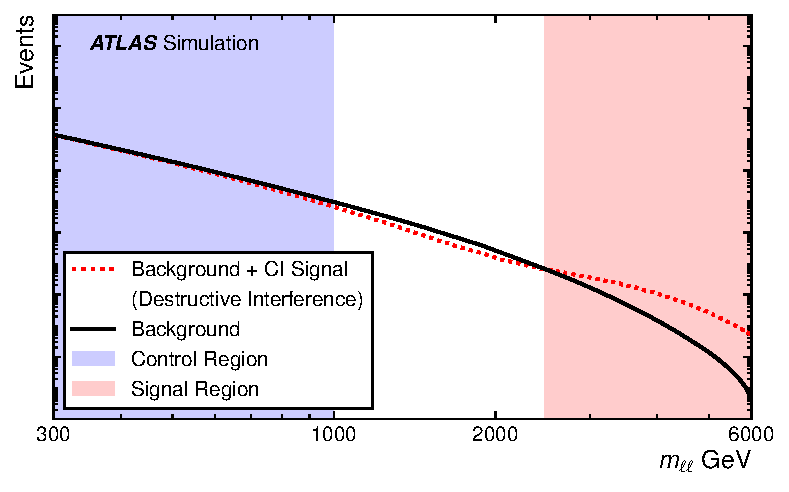
\includegraphics[width=0.99\textwidth]{figures/ci/massRanges.pdf}
\caption{
A schematic example of the dilepton invariant mass spectrum. 
The monotonically falling total background shape is shown by the solid black line, while the dotted red line shows an example of a CI signal plus the total background shape.
A background model is fit to the data it in a low-mass control region (shaded blue area) where a potential bias from the presence of a signal is negligible.
The resulting background shape is extrapolated from the control region into the high-mass signal region (shaded red area).
% The gap illustrated between the CR and the SR is found to be the preferred case for the destructive interference cases only.
}
\label{fig:ciStrat}
\end{figure}

% Challenges
This search for contact interactions is carried out using the dielectron and dimuon invariant-mass spectra.
Since CI produce final states of the same topology as some SM backgrounds, the signal production interferes either constructively or destructively with these backgrounds.
In the constructive case, the CI strictly enhances the spectra with a broad non-resonant shape.
In the destructive case, the interference modifies the background spectra as illustrated in Figure \ref{fig:ciStrat}. 
Both types of interference are considered in this analysis.

This search is complicated by both experimental and phenomenological challenges.
It involves probing the highest energy regimes and smallest length scales ever accessed by observation.
The first challenge results from the width of the non-resonant shape of interest, as shown in the red line of Figure \ref{fig:ciStrat}.
This shape is qualitatively similar to the shape of the background, so care must be taken to avoid interpreting an existing signal as background, thereby losing sensitivity to new physics.
The second challenge is the focus on new CI signals that may manifest themselves in the tail of the invariant-mass spectra.
Attention must be paid to systematic uncertainties in this regime, as well as to the relevant resolution of the measured spectra.
The third challenge is in modeling statistical knowledge of the background in signal regions with very low occupancy.
The sensitivity of the analysis is similarly impacted by statistical and experimental uncertainties on the background expectation, as these are of similar magnitude of the background itself.
New techniques are required to properly address these challenges.

% new analysis strategy: data-driven
This analysis introduces a number of changes that depart from previous searches.
The result presented here is the first non-resonant dilepton search at the LHC to use a functional form fit to data to estimate the background, rather than a background estimate derived from simulated events.
This choice removes the dependence of the background on the theoretical assumptions involved in the simulation process.
This is important because these assumptions are both significant and poorly constrained in the high-mass regime.

% Solution: avoid fitting signal shape
The contact interactions that provide a benchmark model predict deviations from the expected gradient of the high-mass tail of the dilepton mass spectrum; the subtlety of this effect could easily be masked by a background description of sufficient flexibility to match the data.
Therefore, the background event distribution at high masses is estimated based on a low-mass control region (CR) where the contribution of the benchmark signals are negligible.
A functional form is fit to the observed data in the CR, and extrapolated to higher masses to model the production rate of background events.
The search is then performed in a high-mass signal region (SR); here, event production by the benchmark signals is predicted to dominate over the background production.
The arrangement of these mass ranges is illustrated in Figure \ref{fig:ciStrat}.
The extrapolation from CR to SR avoids fitting the data in the regime where CI signals could potentially perturb the fit.
This strategy reduces the impact of a signal shape, if present in the data, on the fitted background model.

% Solution: avoid resolution, etc
ATLAS measures electron transverse energy, \et, and muon transverse momentum, \pt.
Consequently the invariant-mass resolution of dielectron pairs depends on \et resolution.
For high-\et electrons, this grows as a constant fraction of \et. 
Meanwhile, the invariant-mass resolution of dimuon pairs depends on \pt.
As a result, the fractional muon resolution grows linearly with \pt.
Both of these resolutions propagate to their respective invariant-mass spectra.
A single-bin SR is used to combat the effects of these resolutions, which are particularly impactful in the high-mass regime.
All events falling within the SR are counted identically, which mitigates the importance of \et and \pt resolution.
This approach has the additional benefit of removing shape information in the signal region, making the results readily reinterpretable for signal models predicting different non-resonant shapes.

% new analysis strategy: Bayesian
A key part of this analysis is the statistical treatment of the observations.
The Bayesian statistics used in previous ATLAS and CMS searches for CI has been replaced frequentist statistical framework.
This removes the dependence of the result on prior probabilities to observe a signal.
If the interference between signal and SM processes is not negligible, as is the case for CI, the choice of one prior over another is poorly motivated~\cite{Aad:2012hf,EXOT-2016-05}.
% The choice to analyse the observations using frequentist statistics produces in more robust results.

Finally, the transition to a background estimation from the data exchanges the systematic uncertainties in theoretical predictions for statistical uncertainties in data.
There are three new uncertainties that arise from this approach.
The dominant uncertainty in the expected background is due to statistical fluctuations in the CR.
Next in importance is the uncertainty in the degree to which the extrapolation from the CR can produce a background estimate different from the underlying distribution. Such a difference leads to a signal-like deflection in the SR. This uncertainty is quantified using the simulated background and the associated uncertainties.
The third and smallest uncertainty describes the impact of potential signal contamination in the CR.

Two signal regions are considered for each lepton flavor, leading to four signal regions in total.
For each flavor, the first SR extends to relatively lower invariant-mass and targets CI that interfere constructively with the SM.
The second SR remains at relatively high invariant-mass and targets CI that interfere destructively with the SM.
For the latter case, a gap is left between the CR and SR in order to avoid counting the destructive interference in the SR, as illustrated in Figure \ref{fig:ciStrat}.

A statistical analysis is performed on the observation in each SR.
The first results of the analysis are limits on the \xsbr in each SR, which can readily be reinterpreted in terms of various new physics models, without limitation to contact interactions.
This result is the first of its kind, and is a new development for non-resonant searches at the LHC.
The second result uses these four signal regions to set limits on CI models.
These are produced to be reinterpretable in terms of arbitrary CI models \cite{chala}.
The results of this analysis were published on November 4, 2020 \cite{ciAaron}.

% Chapter outline
This chapter describes the ATLAS search for contact interactions using the Run~2 dataset.
Section \ref{sec:ciMotivation} discusses the theoretical motivation.
Section \ref{sec:ciEvSel} describes the selection of data used for the search.
Sections \ref{sec:ciSig} and \ref{sec:ciBkg} present the signal and background models, respectively.
Next Section \ref{sec:ciSyst} discusses the systematic uncertainties used in the result.
Section \ref{sec:ciStat} details the statistical analysis of the data.
Finally Section \ref{sec:ciResults} presents the results and Section \ref{sec:ciConclusion} summarizes the analysis.

\section{Theoretical Motivation for Non-resonance Signatures}\label{sec:ciMotivation}

The effects of a new interaction may be observed at an energy much lower than that required to produce direct evidence of the existence of a new gauge boson.
The charged weak interaction responsible for nuclear $\beta$ decay provides such an example.
A non-renormalizable description of this process was formulated by Fermi in the form of a four-fermion contact interaction~\cite{Fermi:1934hr}.
A CI can also describe deviations from the SM in proton--proton scattering due to quark and lepton compositeness, where a characteristic energy scale \lam corresponds to the binding energy between fermion constituents.
The following Lagrangian can describe a generic \llqq contact interaction, including fermion compositeness \cite{eichten, Eichten:1984eu};
% A new interaction or compositeness in the process $q\overline{q} \to \ell^+\ell^-$ can be described by the following four-fermion contact interaction Lagrangian~\cite{eichten, Eichten:1984eu},

\begin{equation}\label{eqn:ciLagrangian}
\begin{array}{r@{\,}c@{}c@{\,}l@{\,}l}
\mathcal L = \frac{g^2}{2\Lambda^2}\;[ && \eta_{\mathrm{LL}}&\, (\overline q_{\mathrm L}\gamma_{\mu} q_{\mathrm L})\,(\overline\ell_{\mathrm L}\gamma^{\mu}\ell_{\mathrm L}) \nonumber \\
& +&\eta_{\mathrm{RR}}& (\overline q_{\mathrm R}\gamma_{\mu} q_{\mathrm R}) \,(\overline\ell_{\mathrm R}\gamma^{\mu}\ell_{\mathrm R}) \\
&+&\eta_{\mathrm{LR}}& (\overline q_{\mathrm L}\gamma_{\mu} q_{\mathrm L}) \,(\overline\ell_{\mathrm R}\gamma^{\mu}\ell_{\mathrm R}) \\
&+&\eta_{\mathrm{RL}}& (\overline q_{\mathrm R}\gamma_{\mu} q_{\mathrm R}) \,(\overline\ell_{\mathrm L}\gamma^{\mu}\ell_{\mathrm L})& ] \: ,\nonumber
\end{array}
\end{equation}

\noindent where $g$ is a coupling constant chosen by convention\footnote{The interested reader may note that this convention, followed in all ATLAS results, may be adjusted by consistent multiplication of \lam.} to satisfy $g^2/4\pi = 1$, \lam is the contact interaction scale, and $q_{\mathrm L,R}$ and $\ell_{\mathrm L,R}$ are left-handed and right-handed quark and lepton fields, respectively.
The parameters $\eta_{ij}$, where $i$ and $j$ may be left (L) or right (R), define the chiral structure of the new interaction.
Different chiral structures are considered by choices of the coefficients $\eta_{ij}$. For example, the left-right model is obtained by setting $\eta_{\mathrm{LR}} = \pm 1$ and $\eta_{\mathrm{RL}} = \eta_{\mathrm{LL}} = \eta_{\mathrm{RR}} = 0$.
Likewise, the left-left (LL), right-left (RL), and right-right (RR) chirality models are correspond to Lagrangians with the corresponding $\eta_{ij}$ set to $\pm 1$, and the remaining $\eta_{ij}=0$.
The sign of $\eta_{ij}$ determines the sign of interference: $\eta_{ij}=-1$ results in constructive interference, while  $\eta_{ij} = +1$ results in destructive with the Standard Model. 

Equation \ref{eqn:ciLagrangian} becomes more specific in the context of \llqq CI searches in dilepton final states at the LHC.
The terms take the form $\eta_{ij}\left(\bar{q}_i\gamma_{\mu}q_i\right)\left(\bar{\ell}_j\gamma^{\mu}\ell_j\right)$, where $q_i$ and $\ell_j$ are the quark and lepton fields respectively.
The differential cross-section for the process $q\bar{q}\rightarrow\ell^+\ell^-$, in the presence of CI, can be separated into the SM DY term plus terms involving the new contact interaction.
% This separation is given in Equation \ref{eqn:cixs}.
\begin{equation}
\frac{\text{d}\sigma}{\text{d}m_{\ell\ell}} = \frac{\text{d}\sigma_\textrm{DY}}{\text{d}m_{\ell\ell}} - \eta_{ij}\frac{F_\textrm{I}}{\Lambda^2} + \frac{F_\textrm{C}}{\Lambda^4}
\label{eqn:cixs}
\end{equation}
In Equation \ref{eqn:cixs}, the first term accounts for the DY process, the second term corresponds to the interference between the DY and CI processes, and the third term corresponds to the pure CI contribution.
The latter two terms include $F_\textrm{I}$ and $F_\textrm{C}$, respectively, which are functions of the differential cross-section with respect to $m_{\ell\ell}$ with no dependence on \lam~\cite{Eichten:1984eu}.
The interference may be constructive or destructive, and it is determined by the sign of $\eta_{ij}$.

\begin{figure}[htb]
\begin{center}
\begin{equation}
\begin{tikzpicture}
% \draw[style=help lines] (-3,-5) grid (9,2);
\draw (-2,-2) -- (-2,2);
\draw (9.3,-2) -- (9.3,2);
\node (A) at (9.5,1.9) {2};
\begin{feynman}[medium]
    \vertex (p1);
    \vertex [right=3.6em of p1] (p2);
    \vertex [above left=of p1] (qa){\(\phantom{^+}\qbar\)};
    \vertex [below left=of p1] (qb){\(\phantom{^+}q\)};
    \vertex [above right=of p2] (h){\(\ell^{-}\phantom{\qbar}\)};
    \vertex [below right=of p2] (v){\(\ell^{+}\phantom{\qbar}\)};
    \diagram* {
    (qb) --[fermion] (p1) --[fermion] (qa),
    (p1) --[boson,edge label=\(\gamma^*/Z\)] (p2),
    (v) --[fermion] (p2) --[fermion] (h),
    };
\end{feynman}
\node (A) at (10.5em,0) {+};
\begin{feynman}[xshift=17em,medium]
    \vertex [blob] (p1){\(\lam\)};
    \vertex [above left =4.80em of p1] (qa){\(\phantom{^+}\qbar\)};
    \vertex [below left =4.80em of p1] (qb){\(\phantom{^+}q\)};
    \vertex [above right=4.80em of p1] (h){\(\ell^{-}\phantom{\qbar}\)};
    \vertex [below right=4.80em of p1] (v){\(\ell^{+}\phantom{\qbar}\)};
    \diagram* {
    (qb) --[fermion] (p1) --[fermion] (qa),
    (v) --[fermion] (p1) --[fermion] (h),
    };
\end{feynman}
\end{tikzpicture}
\end{equation}
\end{center}
\vspace{-.4cm}
\caption{Leading-order production mechanism for Drell-Yan with additional contact term with scale \lam in the dilepton final state.}
\label{FeynmanCI}
\end{figure}

Contact interactions have motivated a rich set of searches.
Numerous searches for CI have been carried out in neutrino--nucleus and electron--electron scattering~\cite{Anthony:2005pm}, as well as electron--positron~\cite{Abdallah:2008ab, Schael:2006wu}, electron--proton~\cite{Aaron:2011mv}, and proton--antiproton colliders~\cite{Abulencia:2006iv,Abazov:2009ac}.
Searches for CI have also been performed by the ATLAS and CMS Collaborations~\cite{Aad:2014wca, Khachatryan:2014fba}.
The strongest exclusion limits for \llqq CI come from the previous ATLAS non-resonant dilepton analysis conducted using 36.1\fb of \sqrts=13~TeV proton--proton data \cite{Aaboud:2016cth}.
Other ATLAS studies of note include the 2012/2014 search for contact interactions using \sqrts=7/8~TeV collisions at ATLAS \cite{EXOT-2013-19, EXOT-2012-17}.

\section{Dilepton Event Selection}\label{sec:ciEvSel}
The present search is concerned with collisions that produce pairs leptons.
This section lists selection criteria used to identify such events.
% from the dataset collected during Run~2 of the LHC.
The observed dataset, which consists of the events collected by ATLAS during  Run~2 of the LHC, is detailed along with the corresponding simulated background and signal datasets.
% Finally, comparisons between the recorded data and simulation are provided.


\subsection{Event Selection}
During Run~2, roughly $10^{16}$ proton collisions took place inside the ATLAS experiment.
The majority of these events are uninteresting for the purpose of this analysis, so only events meeting appropriate criteria are considered.
This reduces the total number of data events considered for the analysis to 754,870 dimuon events and 883,594 dielectron events.

% GRL
Only events recorded during good operation of the detector are used.
The events meeting this requirement comprise the Good Run List, summarized in Section \ref{sec:physData}.

% Trigger
The first requirement for an event to be considered is the trigger: only events identified as interesting by the ATLAS trigger system are recorded.
The triggers used during data collection differ from year to year. 
In the dielectron channel, the following trigger requirements are applied.
\begin{itemize}
	\item 2015: Two electrons with $\et>12$~GeV,
	\item 2016: Two electrons with $\et>17$~GeV,
	\item 2017 and 2018: Two electrons with $\et>24$~GeV.
	% \item 2015: 2e12\_lhloose\_L12EM10VH
	% \item 2016: 2e17\_lhvloose\_nod0
	% \item 2017 and 2018: 2e24\_lhvloose\_nod0
\end{itemize}
Although events passing these triggers are expected to contain two electrons, both may not be reconstructed after the event is fully processed. 
Therefore, subsequent criteria require at least two electrons to be reconstructed.

In the dimuon channel, the following trigger requirements are applied.
\begin{itemize}
	\item 2015: One isolated ($\ptconeThirty/\pt<0.06$) muon with $\pt>26$~GeV, or any non-isolated muon with $\pt>50$~GeV,
	\item 2016, 2017 and 2018: The same requirement, except the isolation uses \ptvarconeMuon.
	% \item 2015: mu26\_imedium or mu50
	% \item 2016, 2017 and 2018: mu26\_ivarmedium or mu50
\end{itemize}
These trigger on events with single isolated muons.
These triggers are used, rather than a muon equivalent to the electron triggers, to increase the trigger's efficiency for dimuon events; the requirement for an event to have two muons is enforced in the later.

% Object selection
After passing the trigger requirement, events are evaluated under selection criteria.
In events where multiple vertices are reconstructed, the vertex with the largest $\sum\pt^2$ defines the \emph{primary vertex}.
Events are required to have at least two Inner Detector tracks associated with the primary vertex.
The first step is to define requirements for which physical objects are to be considered in each event. This step follows the object definitions from Section \ref{sec:physObjects}.
% Many of the terms used here follow the definitions found in that section.

Further requirements are made as to where the objects were reconstructed in the detector. 
This defines the fiducial region in which the search is carried out.
This definition differs for electrons and muons.

Electrons are defined using the \code{Medium} likelihood identification.
They are required to pass \code{Gradient} isolation.
Additionally, they must not be from a dead calorimeter cluster.
An additional \emph{loose selection} for electrons is defined to study the background from objects falsely reconstructed as electrons.
For these electrons, the \code{LooseAndBLayer} LH identification replaces the \code{Medium} LH.
This is otherwise the same as the nominal electron selection.
The kinematic criteria for both electron selections are listed in Table \ref{tab:ciElectronSel}.

\begin{table}[!htb]
\caption{Selection criteria for electrons. Parameters $d_{0}$ and $z_{0}$ are the transverse and longitudinal displacements of the track associated with the electron, and the vertex.}
\begin{center}
    \begin{tabular}[ht]{l l}
    \toprule
    Feature & Criteria \\
    \midrule
    Pseudorapidity range & $(|\eta| < 1.37) \quad || \quad (1.52 < |\eta| < 2.47)$ \\
    Transverse momentum & p$_T$ $>$ 30~GeV \\
    Track impact parameter significance & ${|d_{0}^{BL}|\over\sigma}$ $<$ 5 \\
    Track $z$ displacement & $|\Delta z_{0}^{BL} \sin{\theta}| <$ 0.5~mm \\
    \bottomrule
    \end{tabular}
\end{center}
\label{tab:ciElectronSel}
\end{table}

Muons are defined using the \code{High}-$p_T$ selection working point and must pass the isolation requirement \code{FCTightTrackOnly}.
An additional cut, the bad muon veto, is used to reject muons with poorly measured \pt.
The remaining kinematic criteria for muons are given in Table \ref{tab:ciMuonsSel}.

\begin{table}[ht]
\caption{Selection criteria for muons. Parameters $d_{0}$ and $z_{0}$ are the transverse and longitudinal displacements of the track associated with the muon, and the vertex.}
\begin{center}
    \begin{tabular}[ht]{l l}
    \toprule
    Feature & Criteria \\
    \midrule
    Transverse momentum  & $\pt>30$ GeV\\
    Pseudorapidity range & $|\eta|<2.5$ \\
    Track impact parameter significance & ${|d_{0}^{BL}|\over\sigma}< 3$ \\
    Track $z$ displacement  & $|\Delta z_{0}^{BL} \sin{\theta}| < 0.5~mm$\\
    \bottomrule
    \end{tabular}
\end{center}
\label{tab:ciMuonsSel}
\end{table}

Occasionally, the interaction of a single particle with detectors results in the reconstruction of two particles.
To limit this occurrence, an \emph{overlap removal} scheme removes particles that are suspiciously close to each other.
The criteria are listed in Table \ref{tab:ciOr}.
\begin{table}[ht]
\caption{Overlap removal}
\begin{center}
    \begin{tabular}[ht]{l l l}
    \toprule
    Reject & Against & Criteria \\
    \midrule
    Electron & Electron & Shared ID track, $\pt^1<\pt^2$ \\
    Muon     & Electron & Is calo-muon and shared ID track \\
    Electron & Muon     & Shared ID track \\
    \bottomrule
    \end{tabular}
\end{center}
\label{tab:ciOr}
\end{table}
Further rejection of muons and electrons takes place if a jet is reconstructed within an angular distance $\Delta R<0.4$.
This helps reduce the presence of secondary leptons.

% Event selection
These criteria reduce the full set of recorded events to a subset to consider, and within each event a set of physical objects to analyze.
It remains to determine whether the event is interesting for the purpose of this dilepton analysis.
Only events containing either two electrons or two muons meet this threshold.
Of the same-flavor leptons in the event, the leading and subleading \et (\pt) pair are selected in the electron (muon) channel.
In the muon channel, only pairs of oppositely charged muons are considered. 
In the electron channel, the charge is ignored because bremsstrahlung emission of photons.
Such photons can alter the track of an electron, leading to the mis-identification of its charge.
Finally, a preliminary invariant mass cut of $\mll>130$~GeV is required.
In the case where both a dielectron and dimuon candidate meet these requirements, the dielectron is selected, and the dimuon is discarded.
This choice is made due to the superior resolution for high-\et electrons.

\subsection{Data and Simulation}
% The data yield rate, broken into the different runs and periods for each year, are shown in Figure ~\ref{fig:ciYields}.
% These plots count events after applying the full selections.

% \begin{figure}[ht!]
% \captionsetup[subfigure]{position=b}
% \centering
% \subfloat[][]{{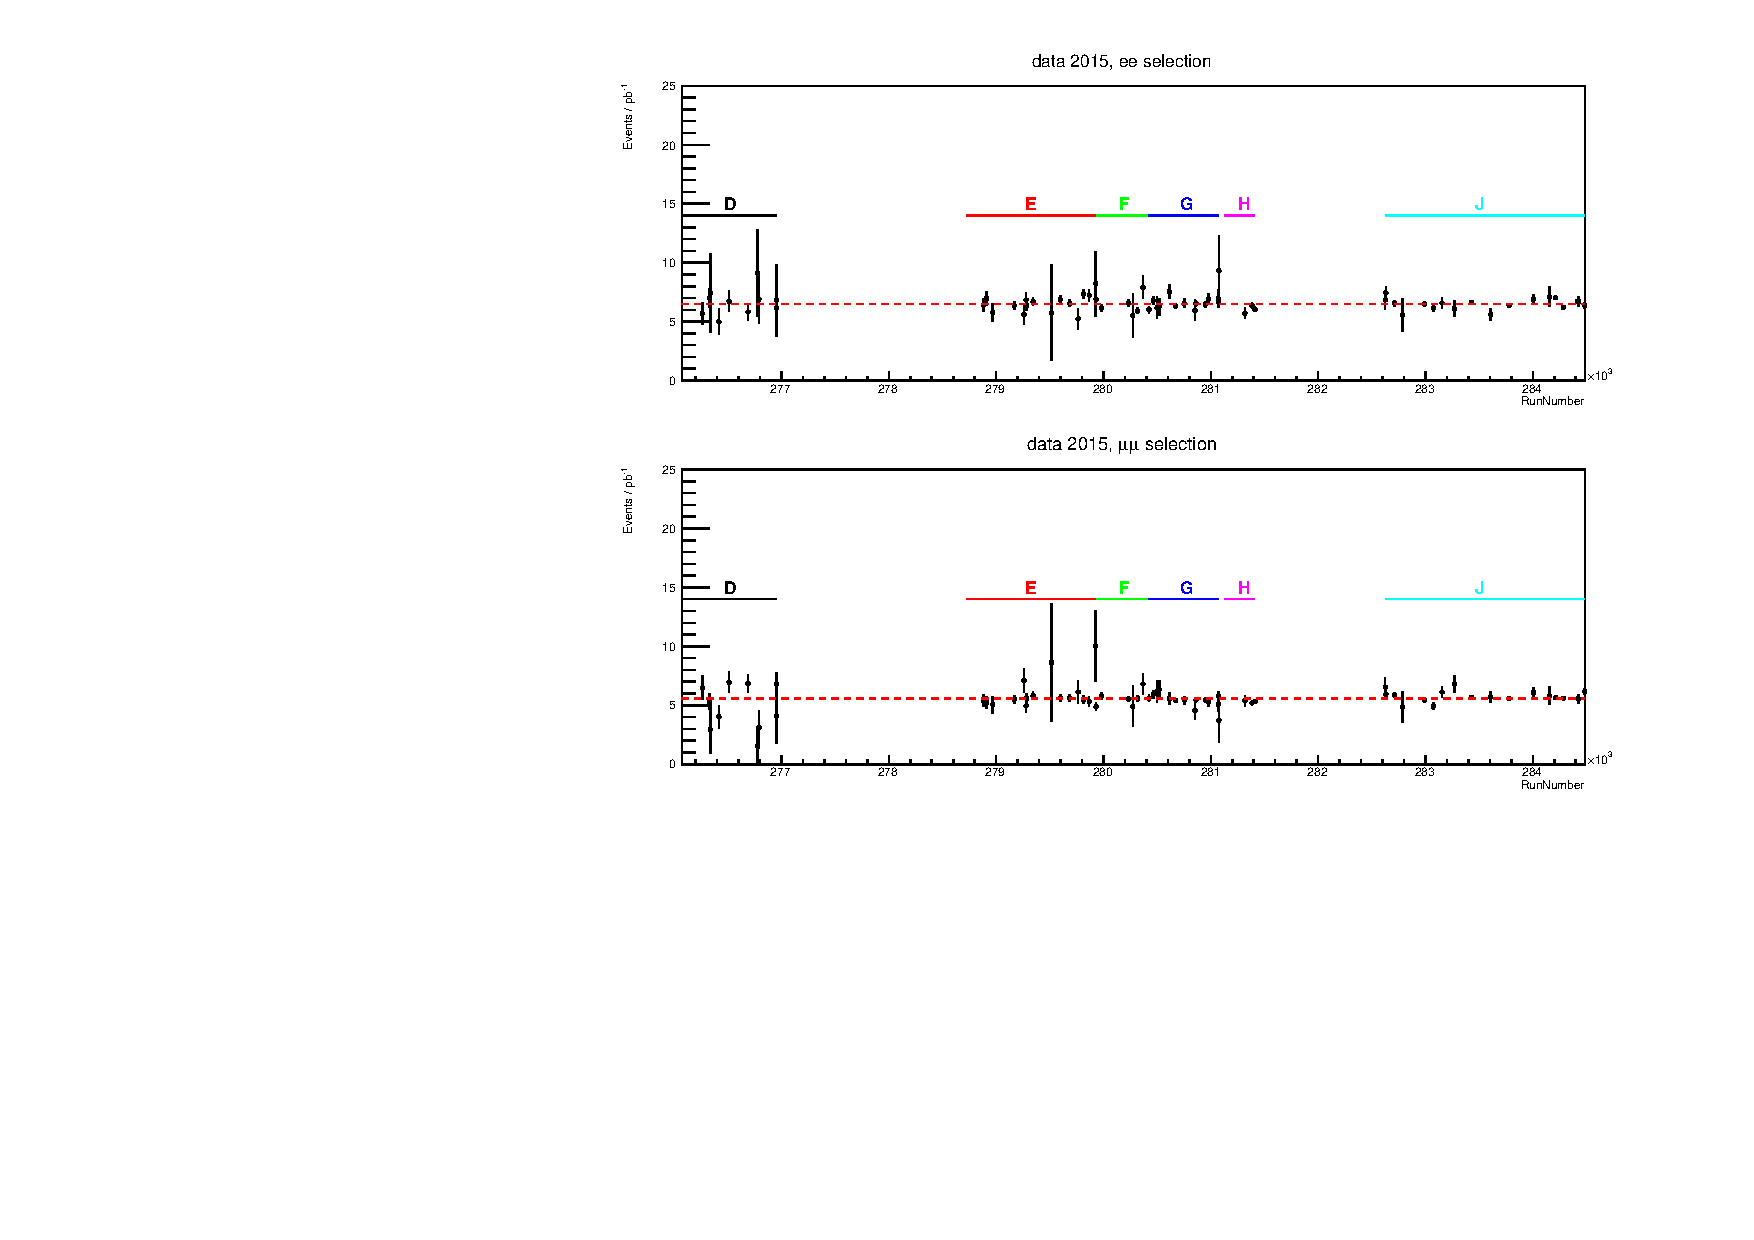
\includegraphics[width=0.48\textwidth]{figures/ci/dataMc/compare_data_yields2015.pdf}}}
% \subfloat[][]{{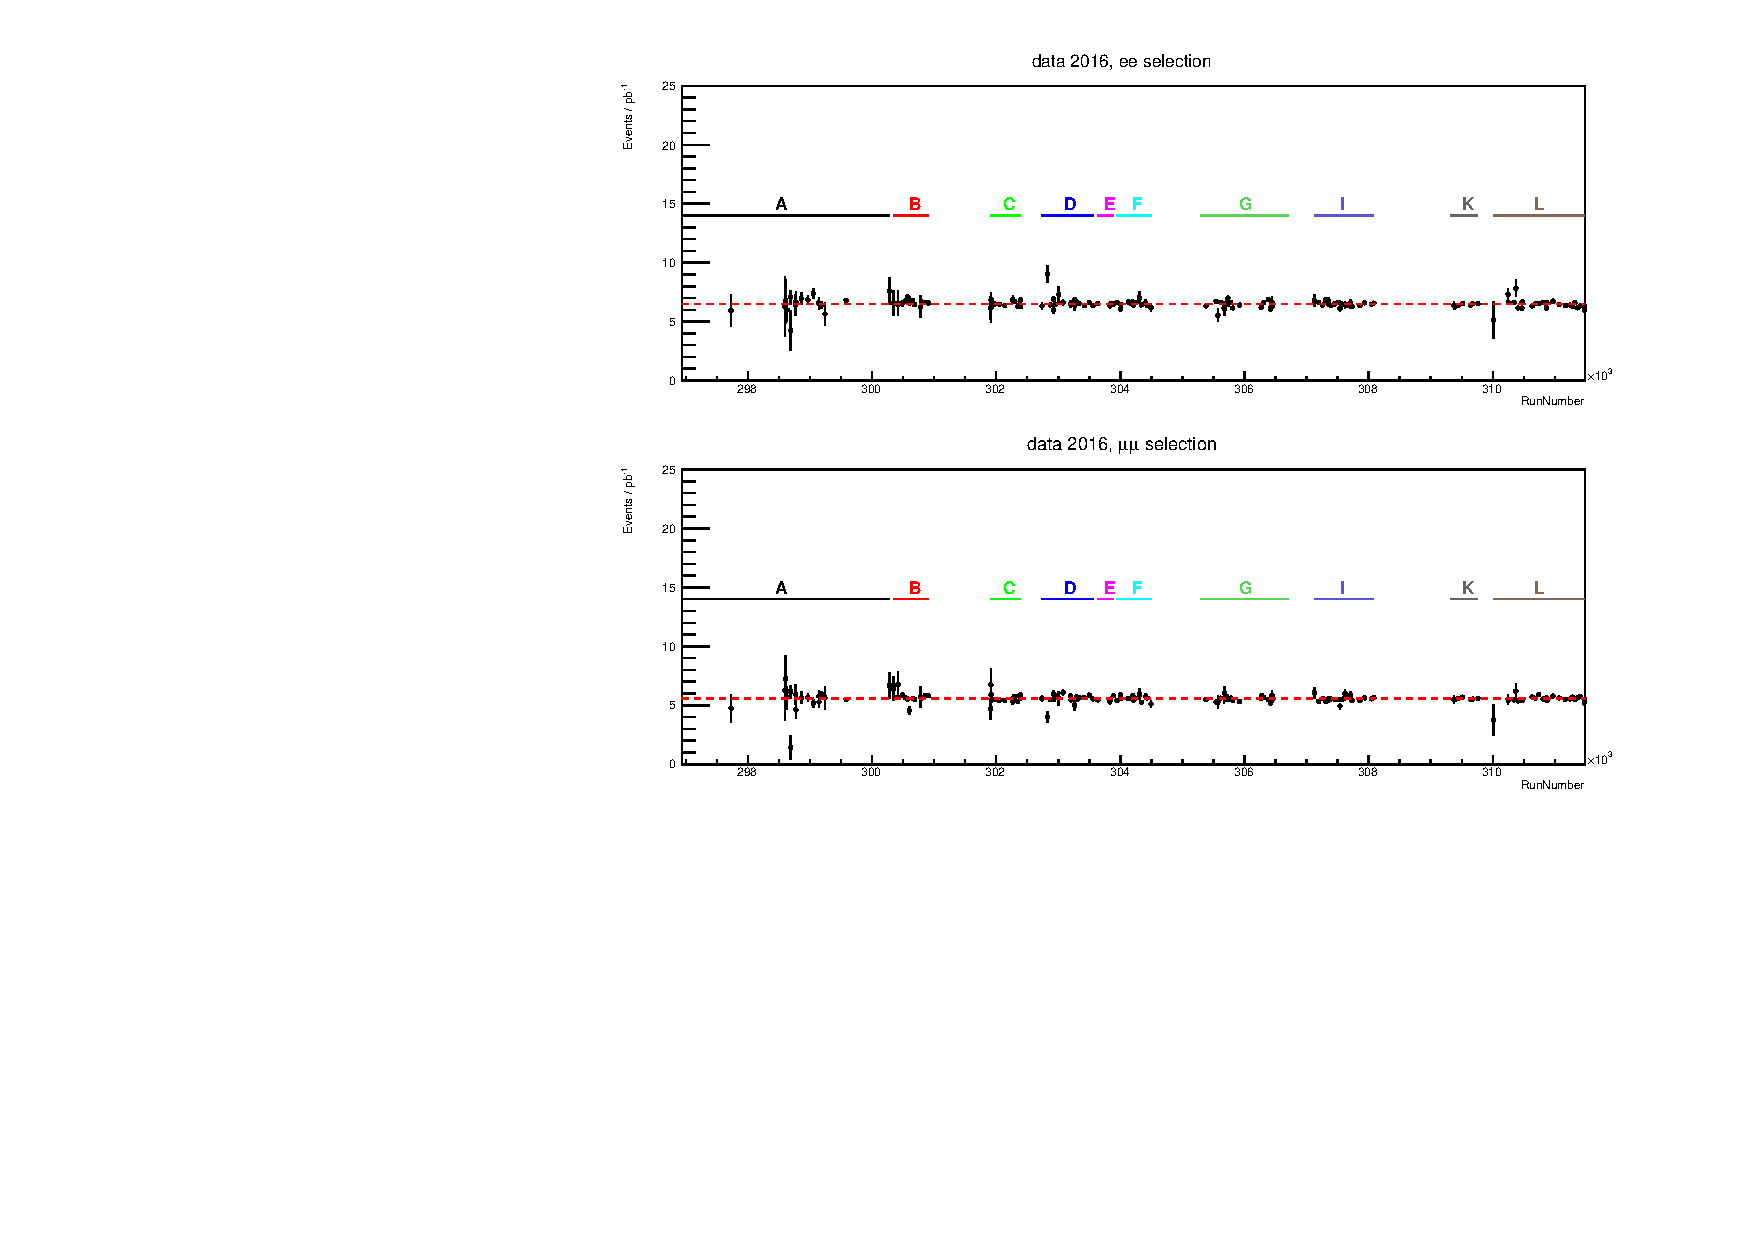
\includegraphics[width=0.48\textwidth]{figures/ci/dataMc/compare_data_yields2016.pdf}}}\\
% \subfloat[][]{{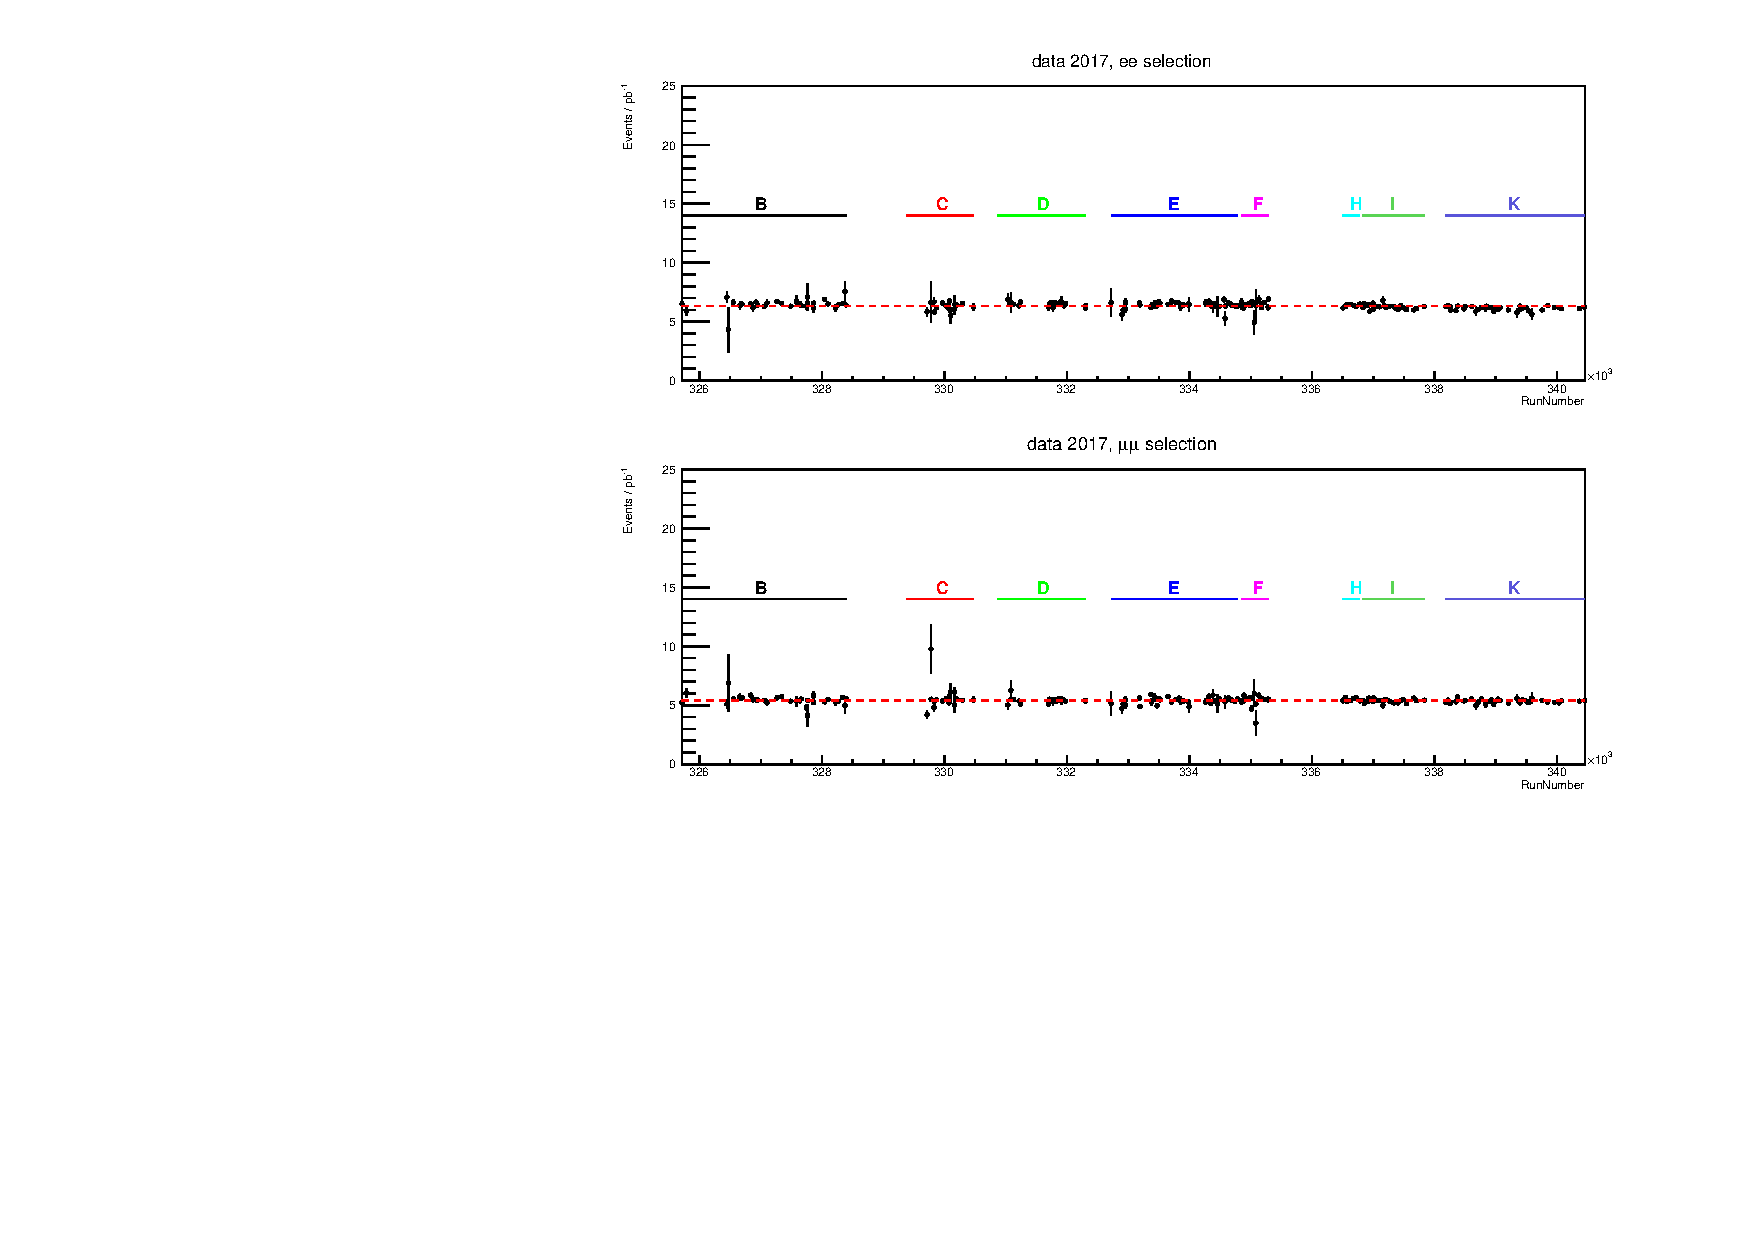
\includegraphics[width=0.48\textwidth]{figures/ci/dataMc/compare_data_yields2017.pdf}}}
% \subfloat[][]{{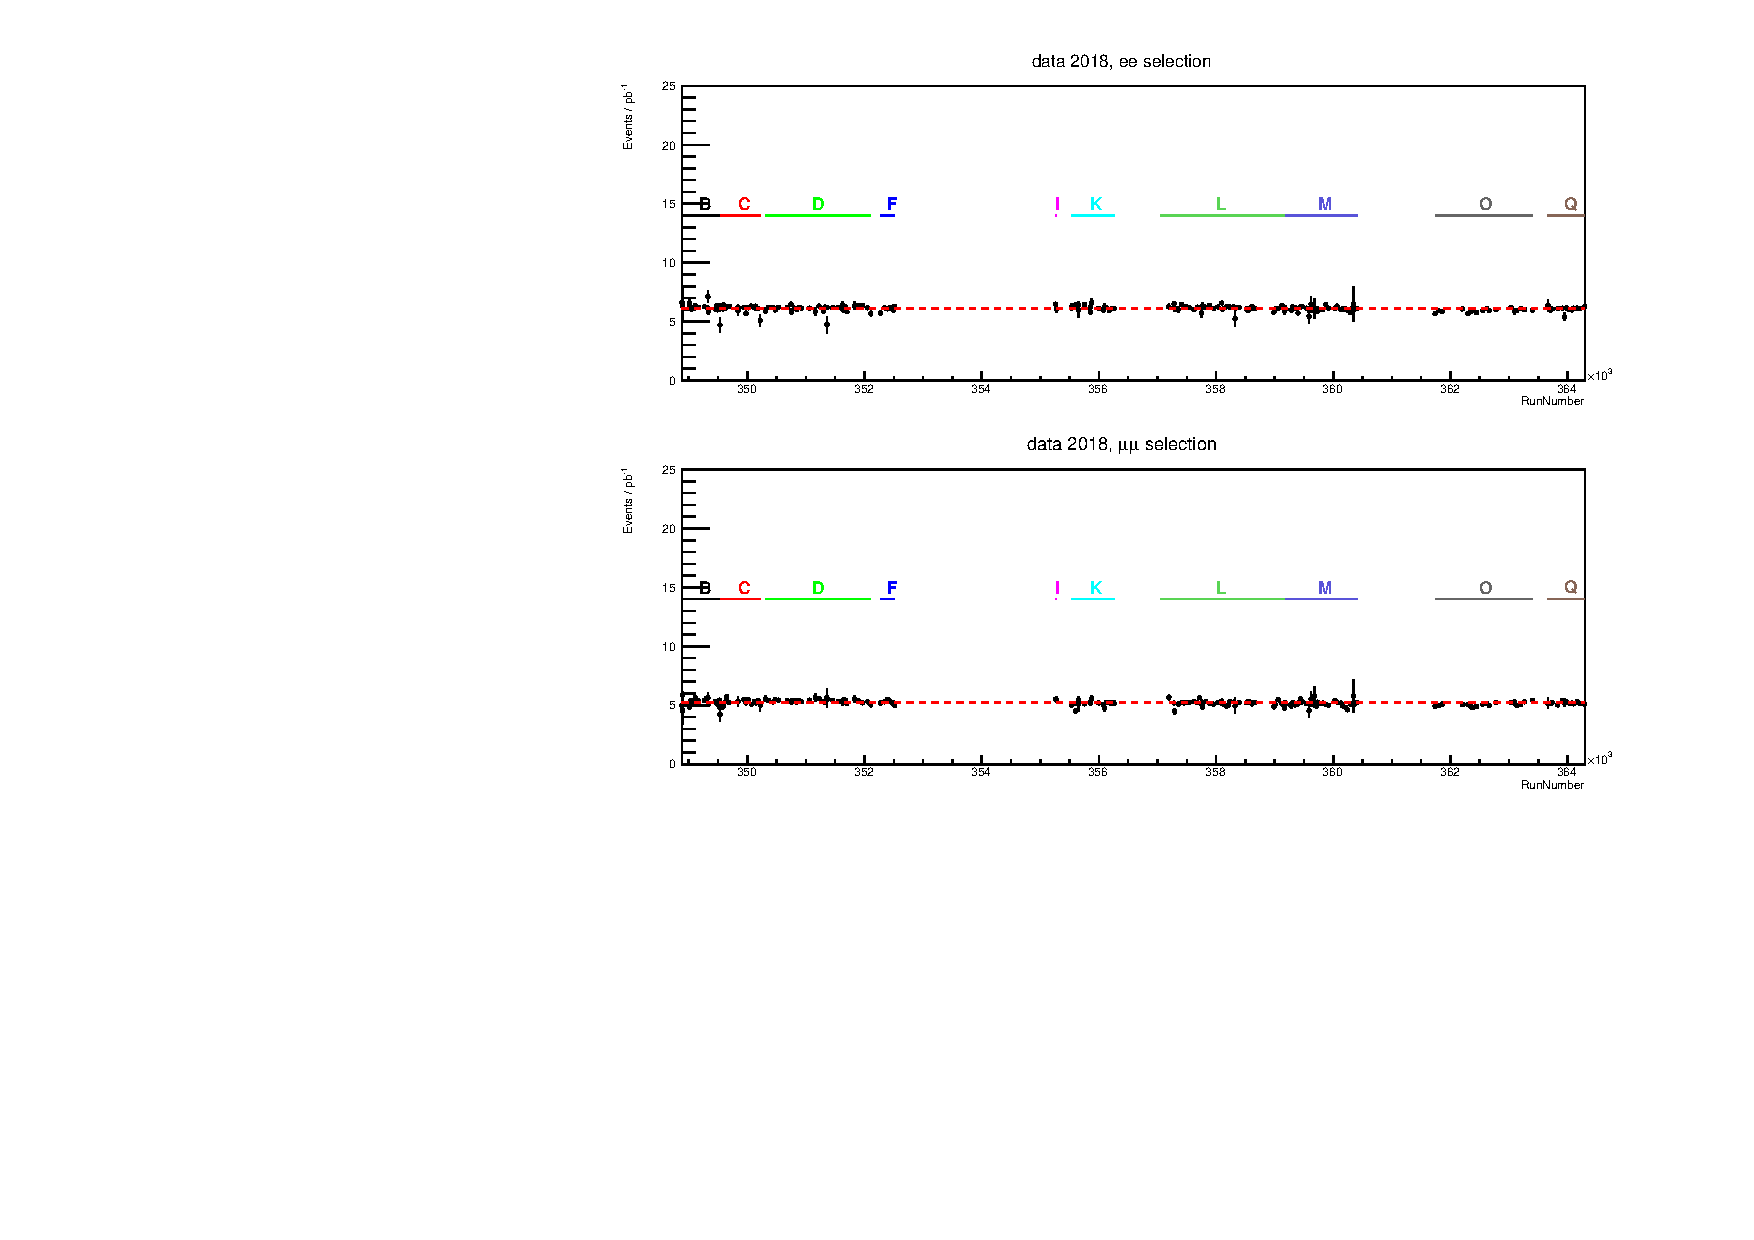
\includegraphics[width=0.48\textwidth]{figures/ci/dataMc/compare_data_yields2018.pdf}}}
% \caption{Data yields for the each run period for the inclusive $ee$ (above) and $\mu\mu$ (below) selections.}
% \label{fig:ciYields}
% \end{figure}
% \clearpage

The data used in this analysis were collected during the LHC Run 2 from \sqrts=13~TeV proton-proton collisions.
The recorded integrated luminosity of the collisions is $139.0\pm2.4$~\fb \cite{ATLAS-CONF-2019-021}.

Despite the reliance on background estimates derived from data, this analysis uses simulated invariant-mass distributions for three purposes.
The first use is to model the CI signal. This is done using simulated DY events, reweighted to include interference and direct production from a contact interaction.
The second use is to test a variety of choices made during the analysis. In particular, the simulation informs the choice of a functional form that matches the expected background shape. Simulation is also used to optimally select the control and signal regions to maximize expected sensitivity while avoiding potential biases.
The third use is to measure the impact of experimental and theoretical uncertainties on the results.

All simulation-based background contributions are scaled by their respective cross-sections and summed to obtain the simulated background invariant-mass distribution.
The main backgrounds in decreasing order of contribution to the full mass spectrum are the Drell--Yan (DY) process, top-quark pair production ($t\bar{t}$), single-top-quark production, and diboson production.
The multi-jet and $W+$jets processes in the dielectron channel are estimated from the data using the matrix method \cite{EXOT-2016-05}. The contribution of such processes to the analysis is estimated using a likelihood fit, and is later treated as an uncertainty in the simulated background.
The same processes in the dimuon channel, as well as processes with $\tau$-leptons in both channels, have been measured to have a negligible impact and consequently are not considered.
The event generators for the hard-scattering process and the programs used for parton showering are listed in Table~\ref{tab:MC} with their respective parton distribution functions (PDFs).
Afterburner generators such as \textsc{Photos}~\cite{Golonka:2005pn} for the final-state photon radiation (FSR) modeling, \textsc{MadSpin}~\cite{Artoisenet:2012st} to preserve top-quark spin correlations, and \textsc{EvtGen}~\cite{Lange:2001uf} for the modeling of $c$- and $b$-hadron decays, are also included in the simulation.

\begin{table}[htbp]
\caption{The programs and PDFs used to generate the hard-scatter matrix element (ME) and to simulate parton showering (PS) in the signal and background processes.
\centering
The top-quark mass is set to 172.5 GeV.}
{\scriptsize
\begin{tabular}{lll}
\toprule
Background Process & ME Generator and ME PDFs & PS and non-perturbative effect with PDFs \\\hline
NLO Drell--Yan & \POWHEGBOX~, CT10~, \textsc{Photos} & \PYTHIAV{v8.186}~, CTEQ6L1~, \textsc{EvtGen1.2.0} \\
$t\bar{t}$  & \POWHEGBOX, NNPDF3.0NLO~ & \PYTHIAV{v8.230}, NNPDF23LO~, \textsc{EvtGen1.6.0} \\
Single top $s$-channel, $Wt$& \POWHEGBOX, NNPDF3.0NLO & \PYTHIAV{v8.230}, NNPDF23LO, \textsc{EvtGen1.6.0} \\
Single top $t$-channel & \POWHEGBOX, NNPDF3.04fNLO, \textsc{MadSpin} & \PYTHIAV{v8.230}, NNPDF23LO, \textsc{EvtGen1.6.0}  \\
Diboson ($WW$, $WZ$ and $ZZ$) & \SHERPA 2.1.1~, CT10 &\SHERPA 2.1.1, CT10  \\\hline
Signal Process & & \\\hline
LO Drell--Yan & \PYTHIAV{v8.186}, NNPDF23LO  &  \PYTHIAV{v8.186}, NNPDF23LO, \textsc{EvtGen1.2.0} \\
LO CI & \PYTHIAV{v8.186}, NNPDF23LO  &  \PYTHIAV{v8.186}, NNPDF23LO, \textsc{EvtGen1.2.0} \\
\bottomrule
\end{tabular}
}
\normalsize
\label{tab:MC}
\end{table}


The DY~\cite{ATL-PHYS-PUB-2016-003} and diboson~\cite{ATL-PHYS-PUB-2016-002} samples were generated in slices of dilepton mass to increase the sample statistics in the high-mass region.
Next-to-next-to-leading-order (NNLO) corrections in QCD and next-to-leading-order (NLO) corrections in EW were calculated and applied to the DY events.
The corrections were computed with {\textsc{VRAP}} v0.9~\cite{vrap} and the CT14 NNLO PDF set~\cite{CT14} in the case of QCD effects, whereas they were computed with {\textsc{MCSANC}}~\cite{MCSANC} in the case of quantum electrodynamic effects due to initial-state radiation, interference between initial- and final-state radiation, and Sudakov logarithm single-loop corrections.
These are calculated as mass-dependent scale factors that are applied to simulated events before reconstruction.
The top-quark samples~\cite{ATL-PHYS-PUB-2016-020} are normalized to the cross-sections calculated at NNLO in QCD, including resummation of the next-to-next-to-leading logarithmic soft gluon terms using \textsc{Top++}2.0 \cite{Czakon:2011xx}.

All fully simulated event samples include the effect of multiple proton interactions in the same or neighboring bunch crossings.
These effects are collectively referred to as pile-up.
The simulation of pile-up collisions was performed with \PYTHIAV{v8.186} using the ATLAS A3 set of tuned parameters~\cite{ATL-PHYS-PUB-2016-017} and the NNPDF23LO PDF set, and weighted to reproduce the average number of pile-up interactions per bunch crossing observed in data.
The generated events were passed through a full detector simulation~\cite{SOFT-2010-01} based on\ \GEANT~4~\cite{geant}.

% Scale factors
The simulated data is weighted by several scale factors (SF) to improve its representation of the observed data.
Pile-up weights are used to describe the effects multiple collisions per beam crossing.
Mass dependant $K$-factors account for differences in the total cross-section if higher-order calculations are available for a given process compared to the order available for simulation. In the case of the LO and NLO DY samples, the SFs provide corrections for higher-order QCD, EW, and photon-induced (PI) effects.
Experimental scale factors for leptons are considered. For electrons, reconstruction, trigger, isolation, and identification scales factors are applied. For muons, reconstruction, trigger, isolation, and track-to-vertex association (TTVA) scale factors are applied.
Trigger scale factors according to the specific channel.

% \begin{itemize}
%     \item Pile-up weights describe the effects multiple collisions per beam crossing.
%     \item Mass dependant $K$-factors account for differences in the total cross-section if higher-order calculations are available for a given process compared to the order available for simulation. In the case of the LO and NLO DY samples, the SFs provide corrections for higher-order QCD, EW, and photon-induced (PI) effects.
%     \item Experimental scale factors for leptons are considered. For electrons, reconstruction, trigger, isolation, and identification scales factors are applied. For muons, reconstruction, trigger, isolation, and track-to-vertex association (TTVA) scale factors are applied.
%     \item Trigger scale factors according to the specific channel.
% \end{itemize}

To reduce statistical uncertainties, a large additional DY sample is used where the detector response is modeled by smoothing the dilepton invariant-mass with mass-dependent acceptance and efficiency corrections, instead of using the computationally expensive \GEANT~4 simulation.
The relative dilepton mass resolution used in the smearing procedure is defined as $(m_{\ell\ell}-m_{\ell\ell}^\mathrm{true})/m_{\ell\ell}^\mathrm{true}$, where $m_{\ell\ell}^\mathrm{true}$ is the generated dilepton mass at Born level before final-state radiation.
The mass resolution is parameterized as a sum of a Gaussian distribution, which describes the detector response, and a Crystal Ball function composed of a secondary Gaussian distribution with a power-law low-mass tail, which accounts for bremsstrahlung effects and for the effect of poor resolution in the muon momentum at high-\pt.
The parameterization of the relative dilepton mass resolution as a function of $m_{\ell\ell}^\mathrm{true}$ is determined by a fit of the function described above to simulated DY events at NLO.
A similar procedure is used to produce a mass-smeared $t\bar{t}$ sample.
These two samples replace the equivalent ones produced with the full detector simulation wherever applicable in the remainder of the analysis.
These samples are composed of over 55 times the number of events in the observed dataset.

Signal \mll distribution shapes are obtained by a matrix element reweighting of the leading-order (LO) DY samples generated in slices of dilepton mass \cite{EXOT-2016-05}.
This reweighting includes the full interference between the non-resonant signal and the background DY process.
The weight function is the ratio of the analytical matrix elements of the full contact interaction (including the DY component) and the DY process only, both at LO precision.
It takes as an input the generated dilepton mass at Born level before FSR, the flavor of the incoming quarks, and the CI model parameters (\lam, chirality states, and the sign of interference).
These weights are applied to the LO DY events to transform these into the CI signal shapes, in steps of $2$~TeV between $\Lambda=12$~TeV and $\Lambda=100$~TeV.
Mass-dependent higher-order QCD production corrections for the signals are computed with the same methodology as for the DY background, correcting from LO to NNLO precision.
Similarly, electroweak corrections for the signals are applied in the CI reweighting along with the interference effects, correcting from LO to NLO precision.
These signal shapes are used for optimizations as well as for calculations of the cross-section and acceptance times efficiency.

The invariant-mass distributions of the simulated datasets, and of the observed data are shown in Figure \ref{fig:ciMassMcPlot}.
Several representative contact interaction shapes imposed on top of the background yields for reference.
These plots clearly show the relative composition of the background in the simulated distributions.
The plots of the \ee selection additionally include the multi-jet and $W+$jets background.

\afterpage{
\begin{figure}[h!]
\captionsetup[subfigure]{position=b}
\centering
 \begin{minipage}[b]{.45\linewidth}
    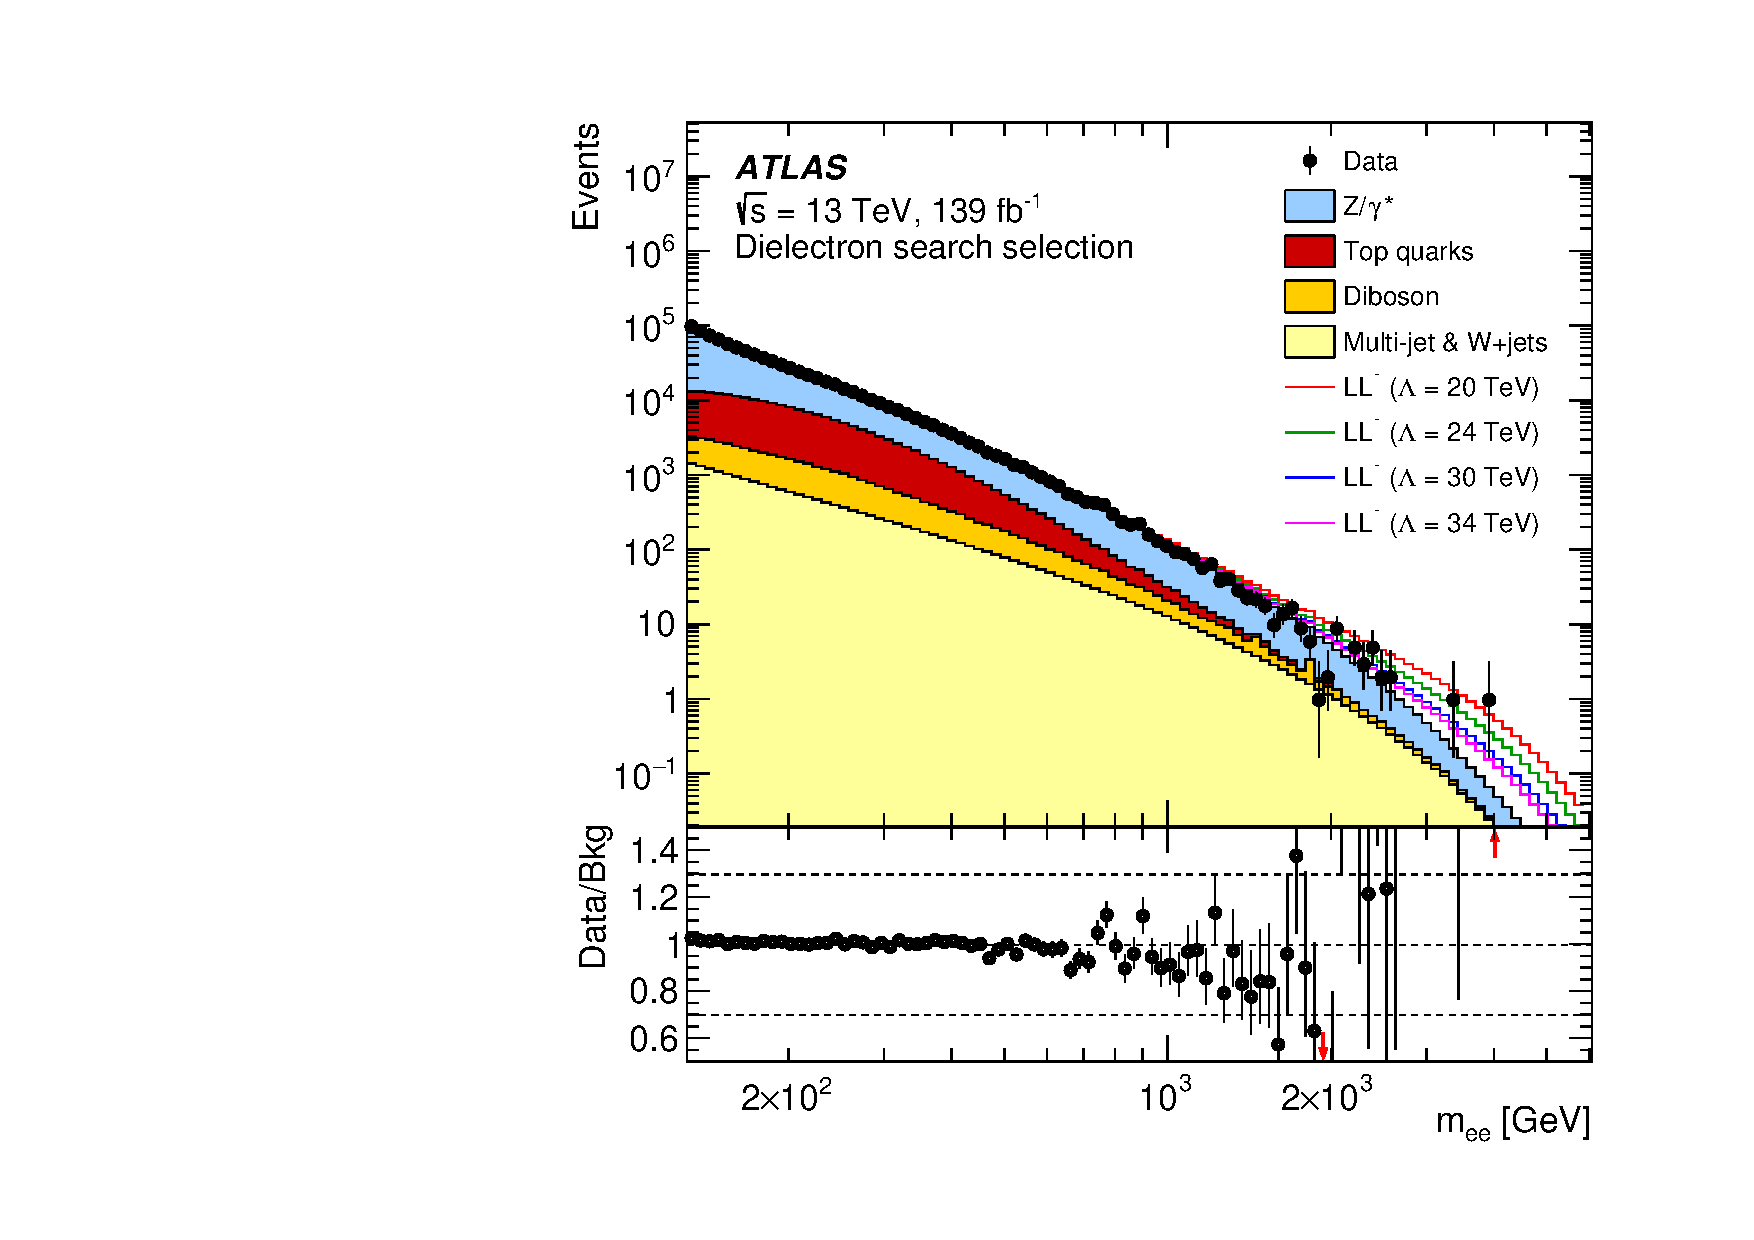
\includegraphics[width=1\textwidth]{figures/ci/dataMc/figaux_05a.pdf}
    \subcaption{}\label{fig:1a}
\end{minipage}
\begin{minipage}[b]{.45\linewidth}
    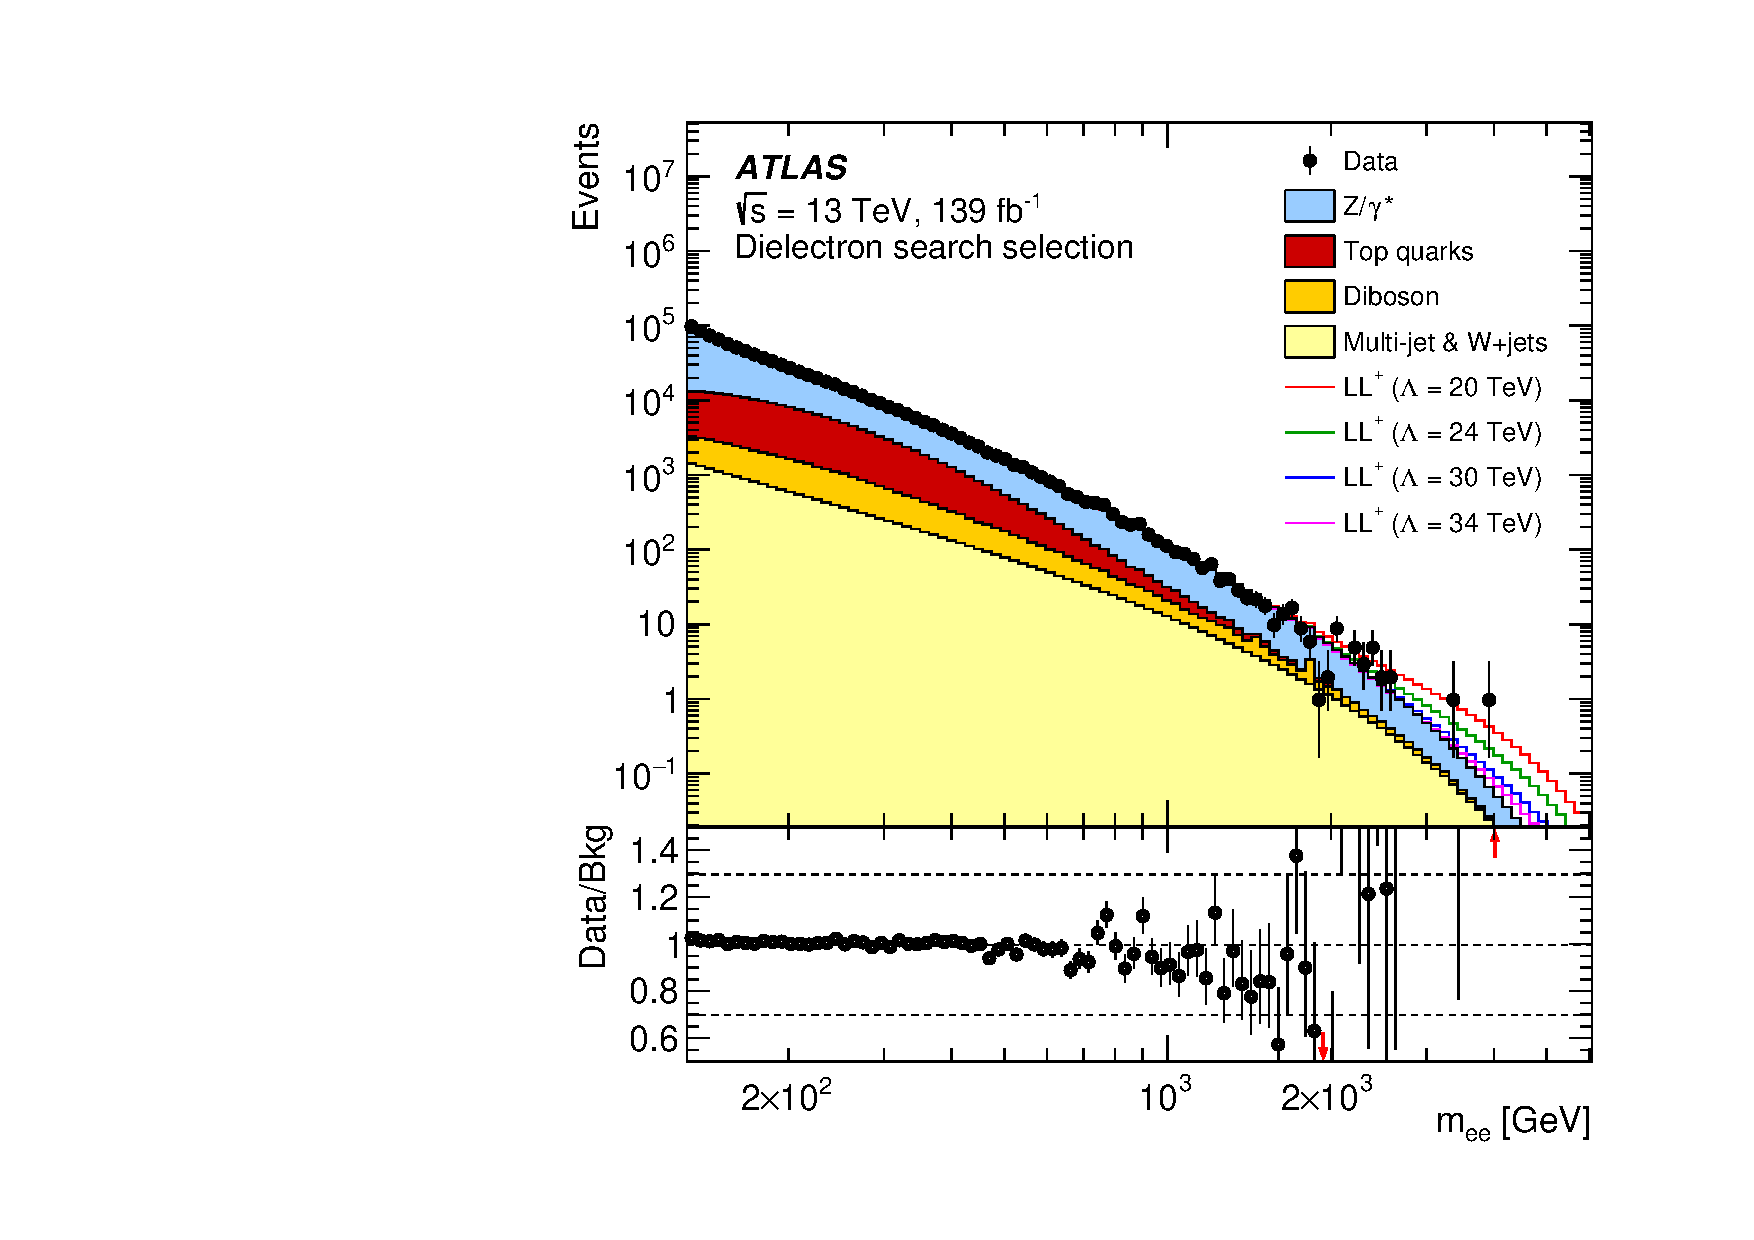
\includegraphics[width=1\textwidth]{figures/ci/dataMc/figaux_05b.pdf}
    \subcaption{}
\end{minipage} \\
\begin{minipage}[b]{.45\linewidth}
    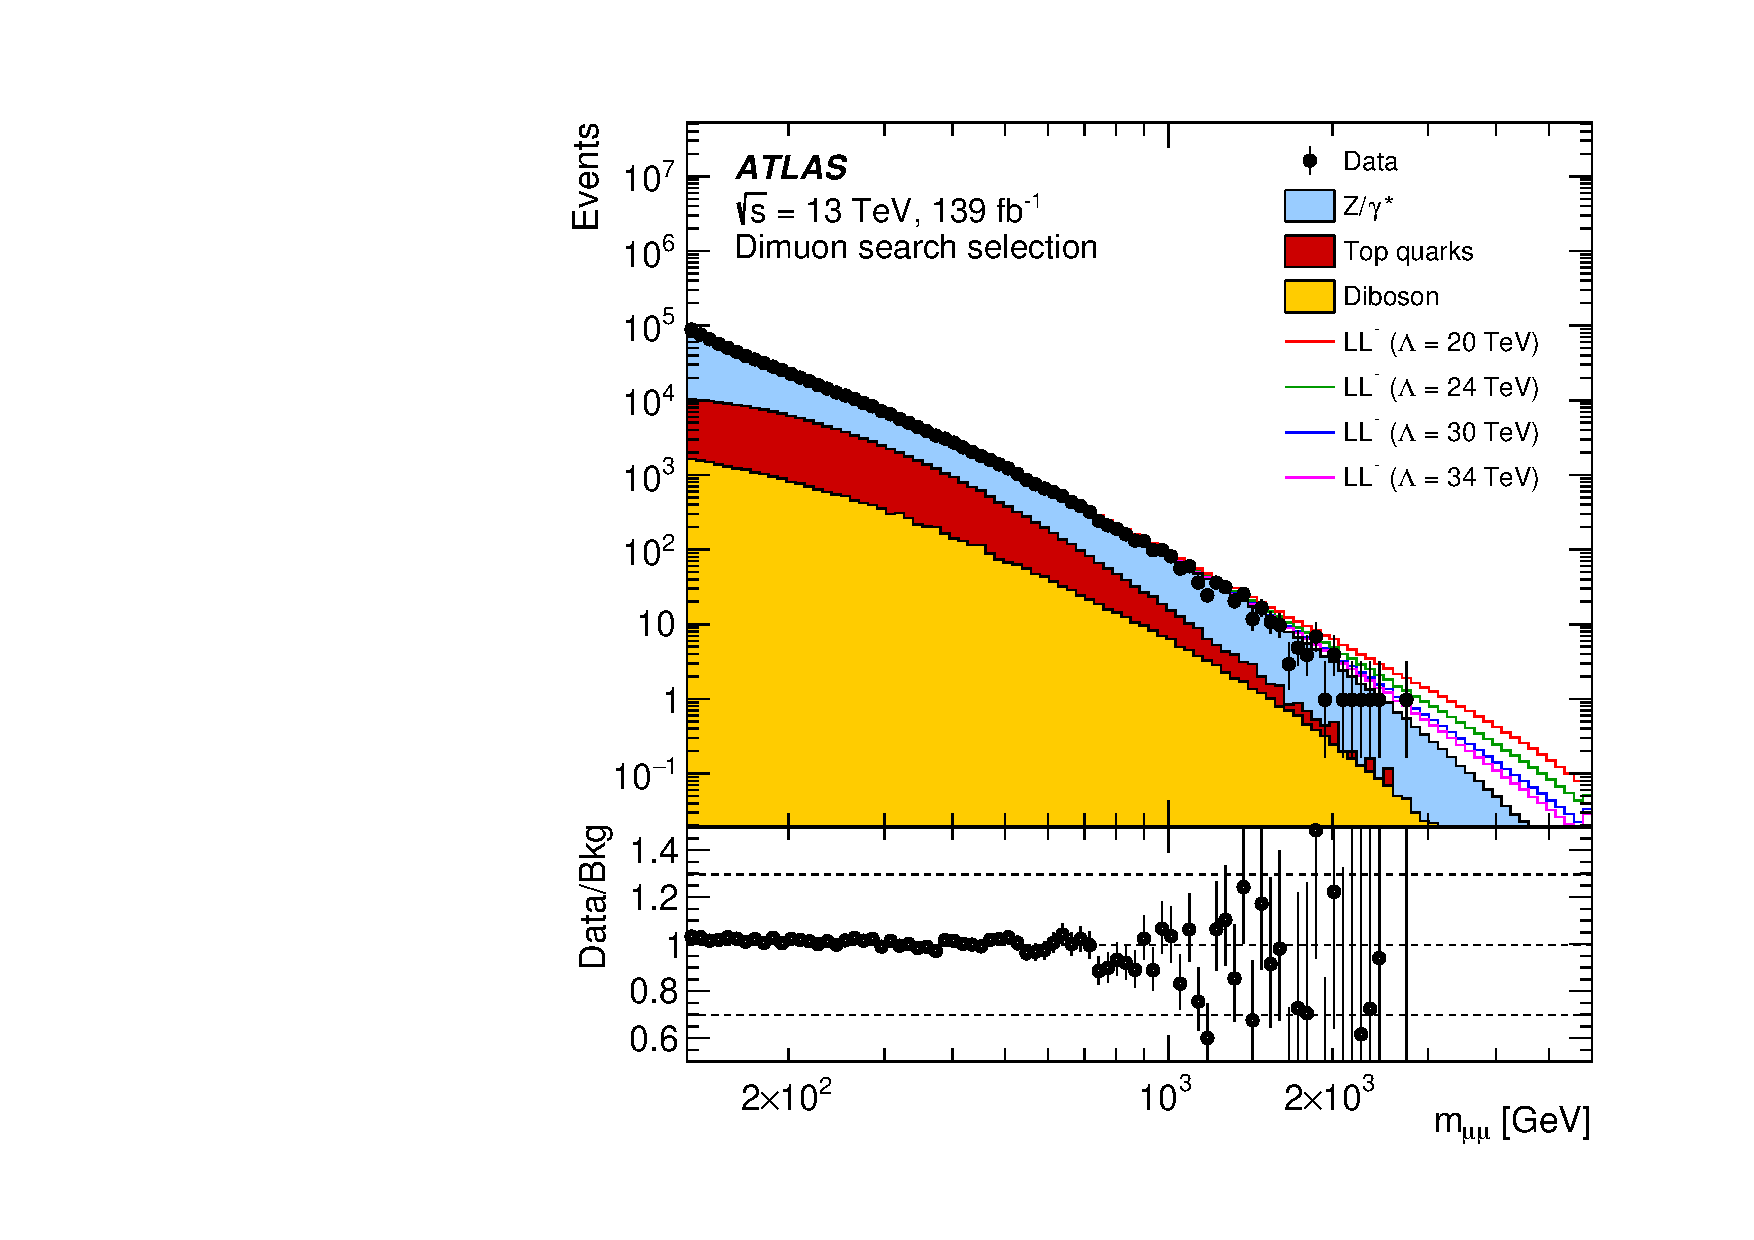
\includegraphics[width=1\textwidth]{figures/ci/dataMc/figaux_06a.pdf}
    \subcaption{}
\end{minipage}
\begin{minipage}[b]{.45\linewidth}
    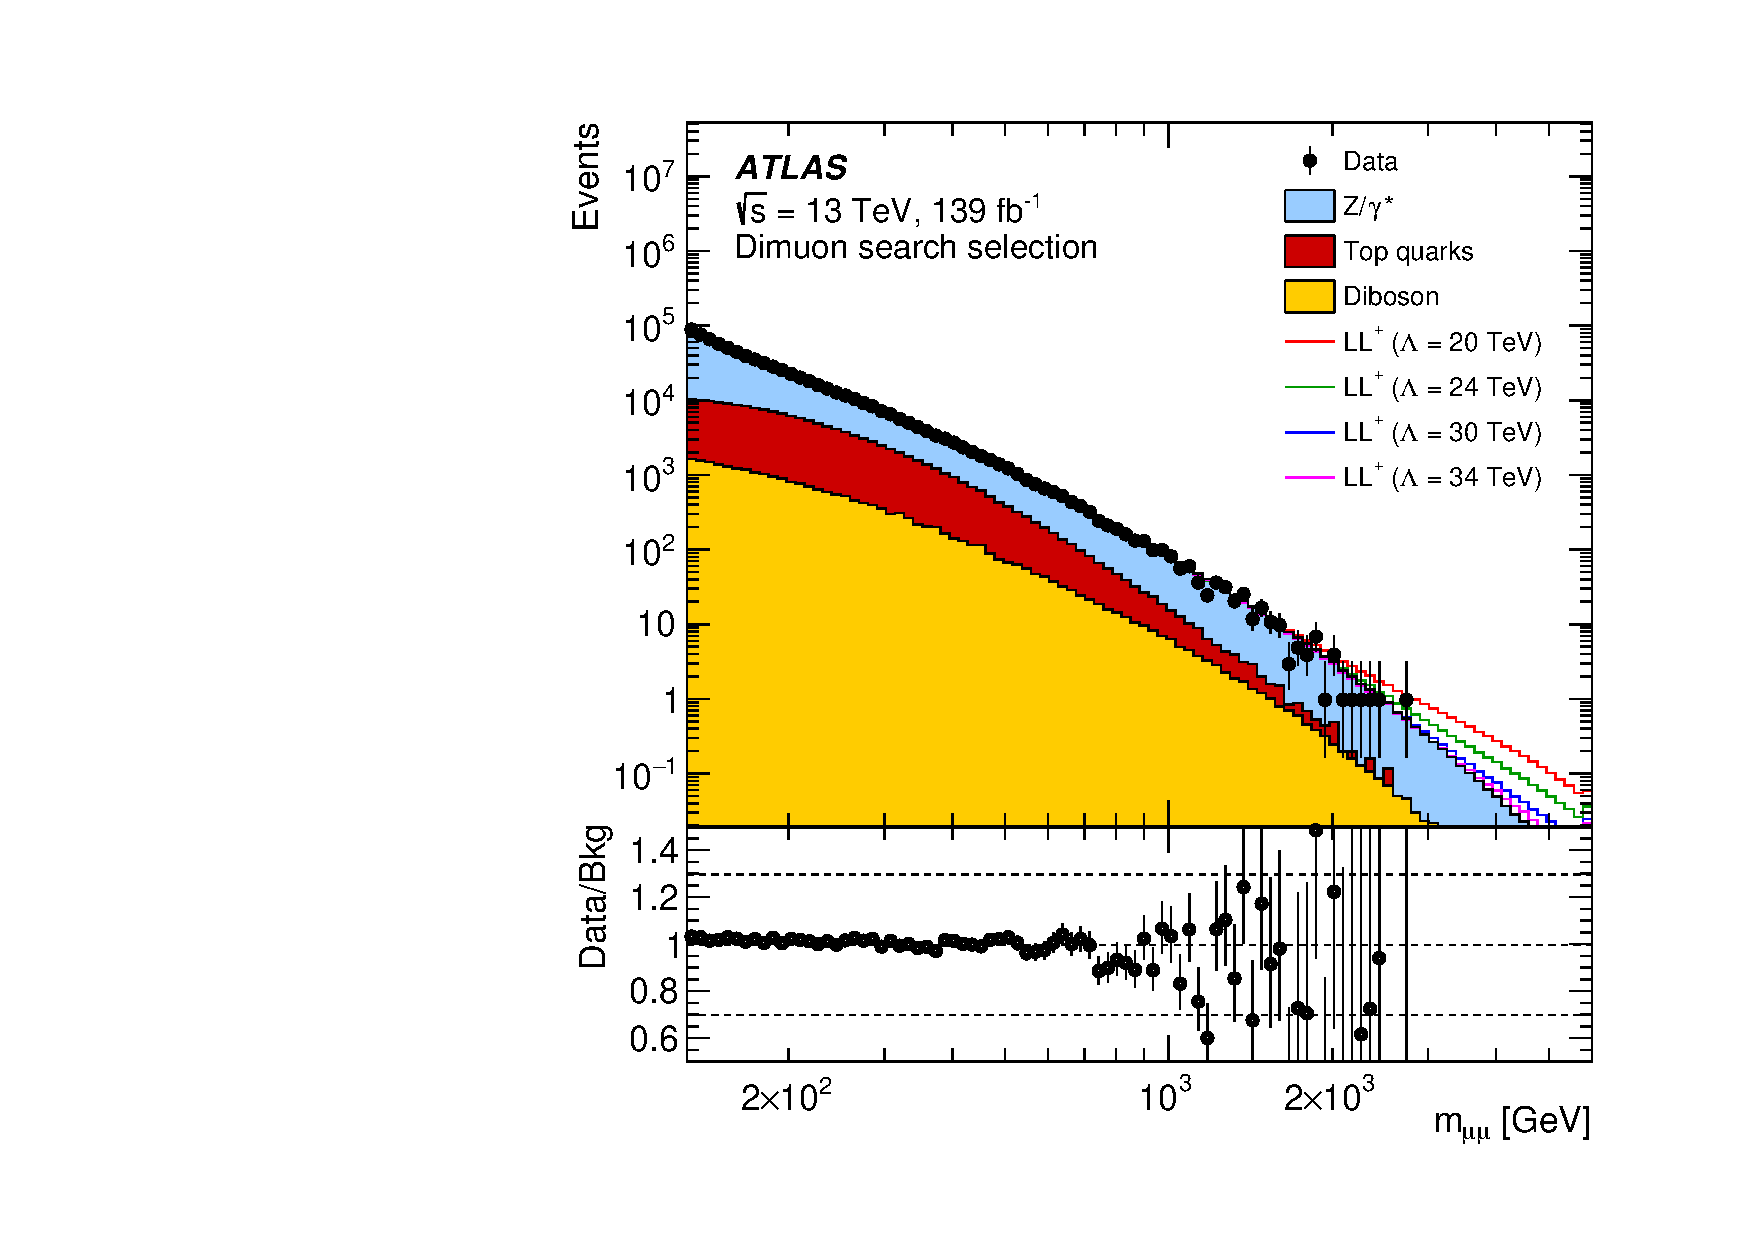
\includegraphics[width=1\textwidth]{figures/ci/dataMc/figaux_06b.pdf}
    \subcaption{}
\end{minipage}
\caption{Invariant-mass distributions in the $ee$ channel (top) and $\mu\mu$ channel (bottom). Plots on the left show selected constructive CI signal shapes imposed on top of the simulated distribution, while plots on the right show the same for destructive CI signal shapes.}
\label{fig:ciMassMcPlot}
\end{figure}
\clearpage
}

% \subsection{Kinematic Distributions}

% Several distributions of kinematic variables are provided in the following figures.
% These plots show the distribution of simulated events along with data events for both \ee and \mm selections.
% The following figures show some kinematic variables for each selection.
% Fully simulated resonant signals are included in these as illustrations, as the CI signal is reweighted only in the invariant-mass distribution.


% \afterpage{
% \begin{figure}[h!]
% \captionsetup[subfigure]{position=b}
% \centering
%  \begin{minipage}[b]{.45\linewidth}
%     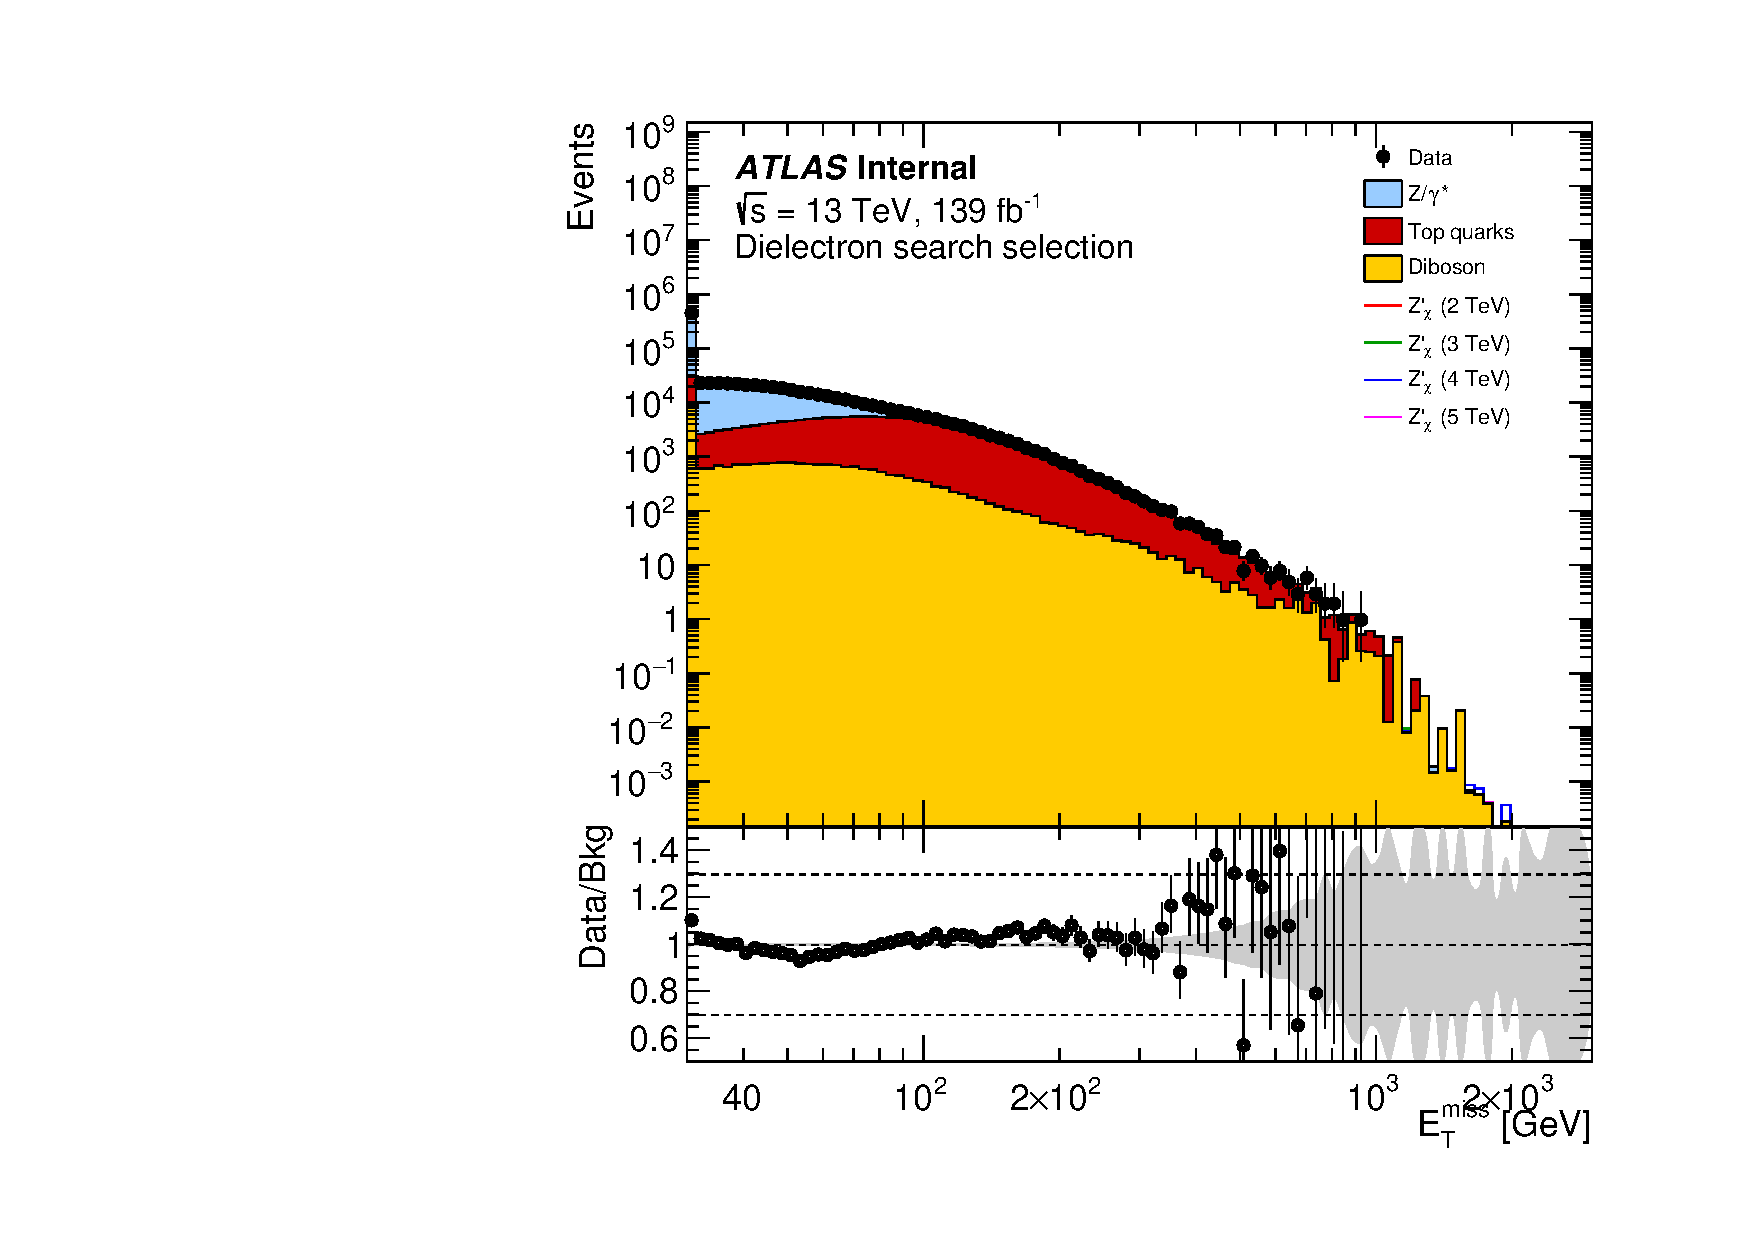
\includegraphics[width=1\textwidth]{figures/ci/dataMc/stacks_mc16e_2015-2018_ee_met_log100.pdf}
%     \subcaption{}\label{fig:1a}
% \end{minipage}
% \begin{minipage}[b]{.45\linewidth}
%     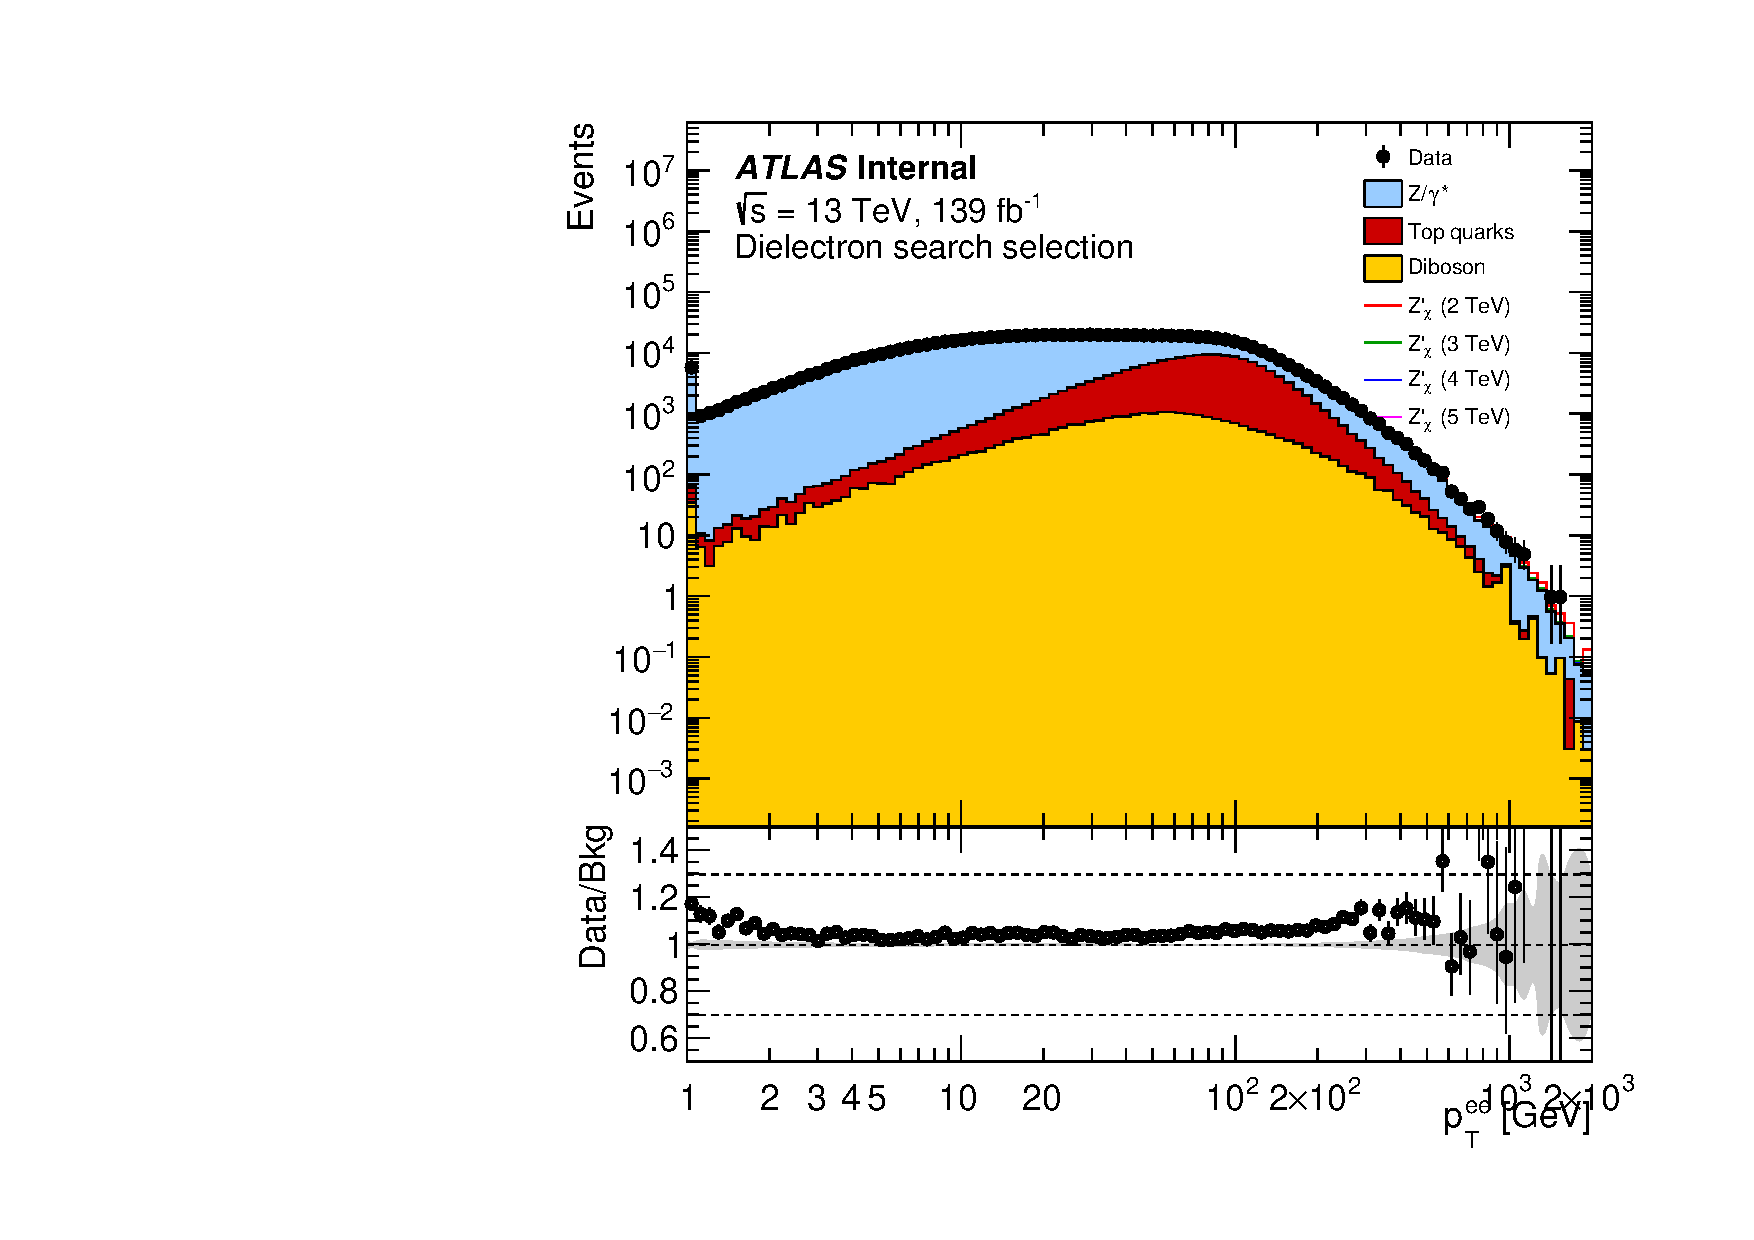
\includegraphics[width=1\textwidth]{figures/ci/dataMc/stacks_mc16e_2015-2018_ee_ptll_log100.pdf}
%     \subcaption{}
% \end{minipage} \\
% \begin{minipage}[b]{.45\linewidth}
%     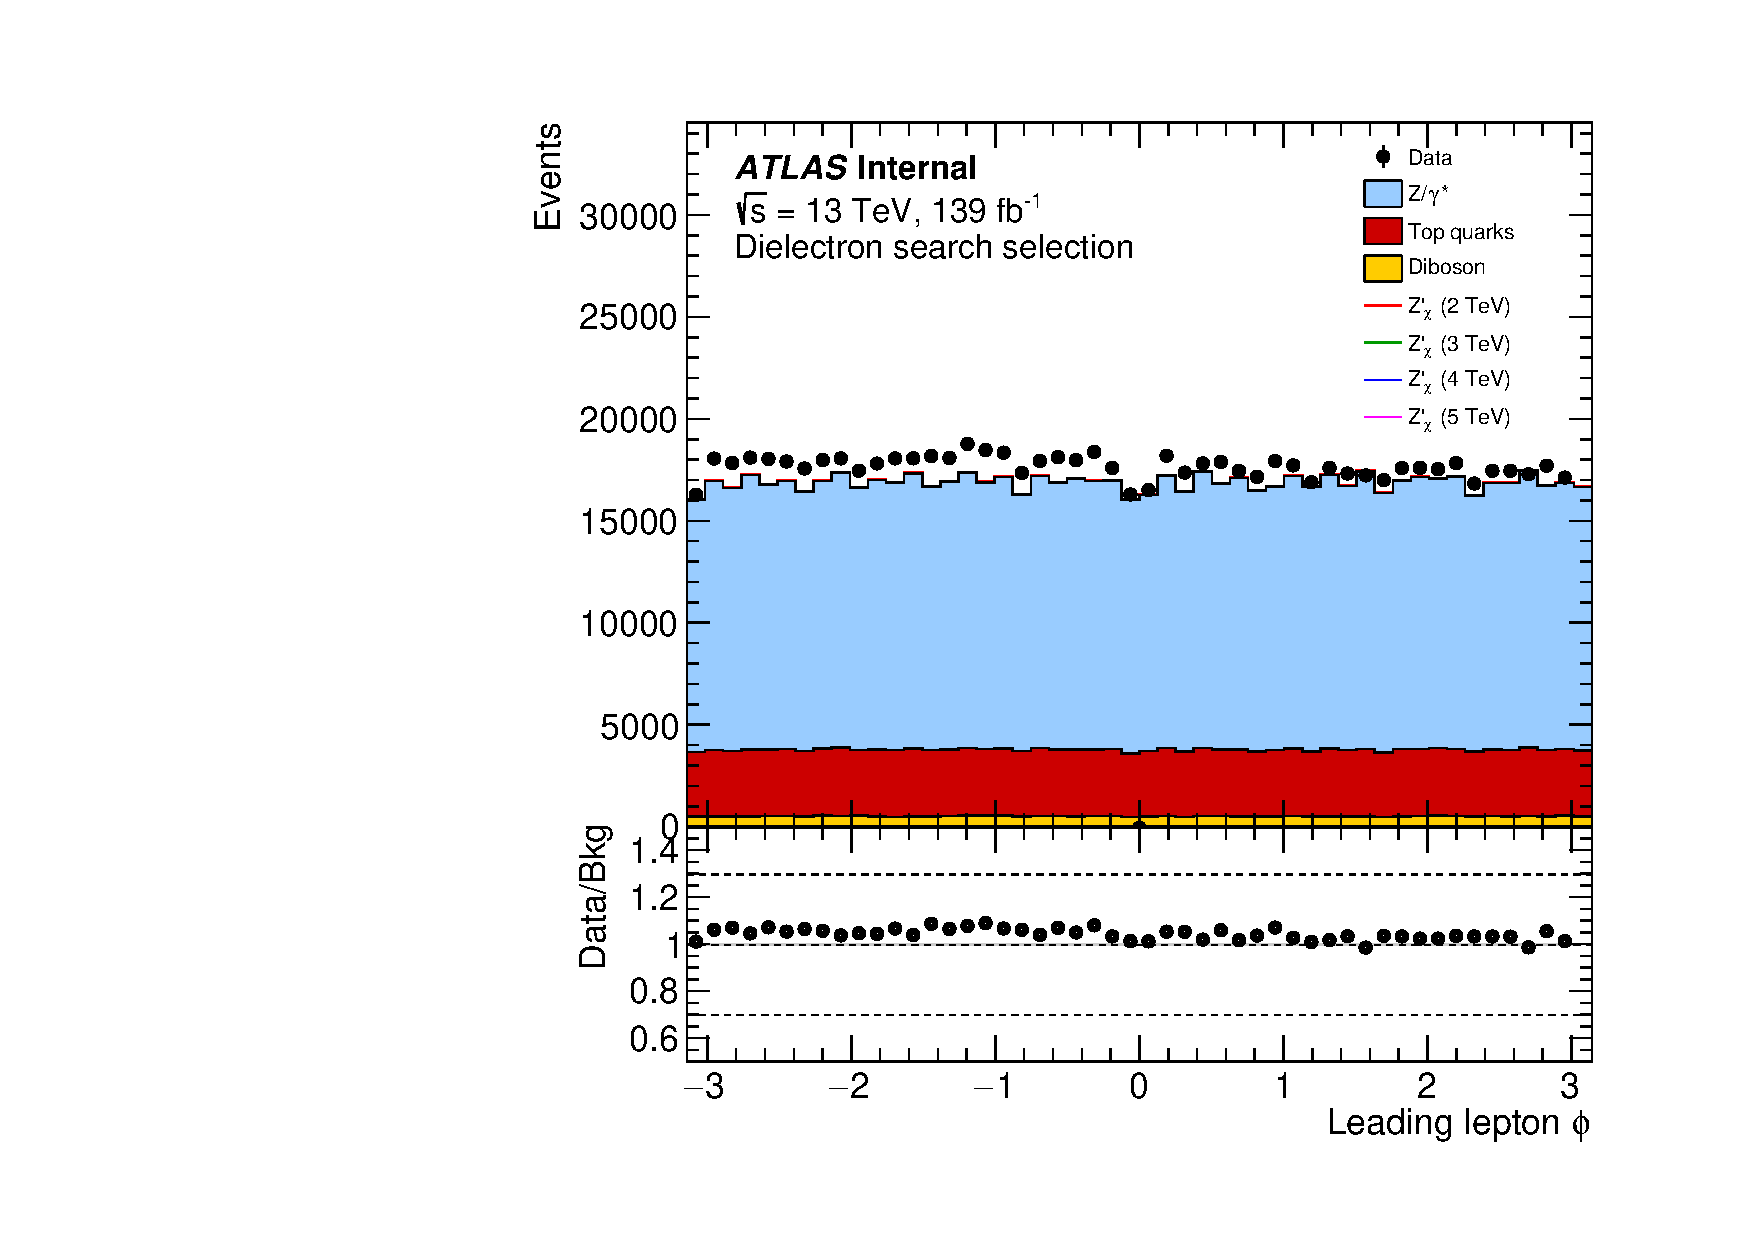
\includegraphics[width=1\textwidth]{figures/ci/dataMc/stacks_mc16e_2015-2018_ee_phi1.pdf}
%     \subcaption{}
% \end{minipage}
% \begin{minipage}[b]{.45\linewidth}
%     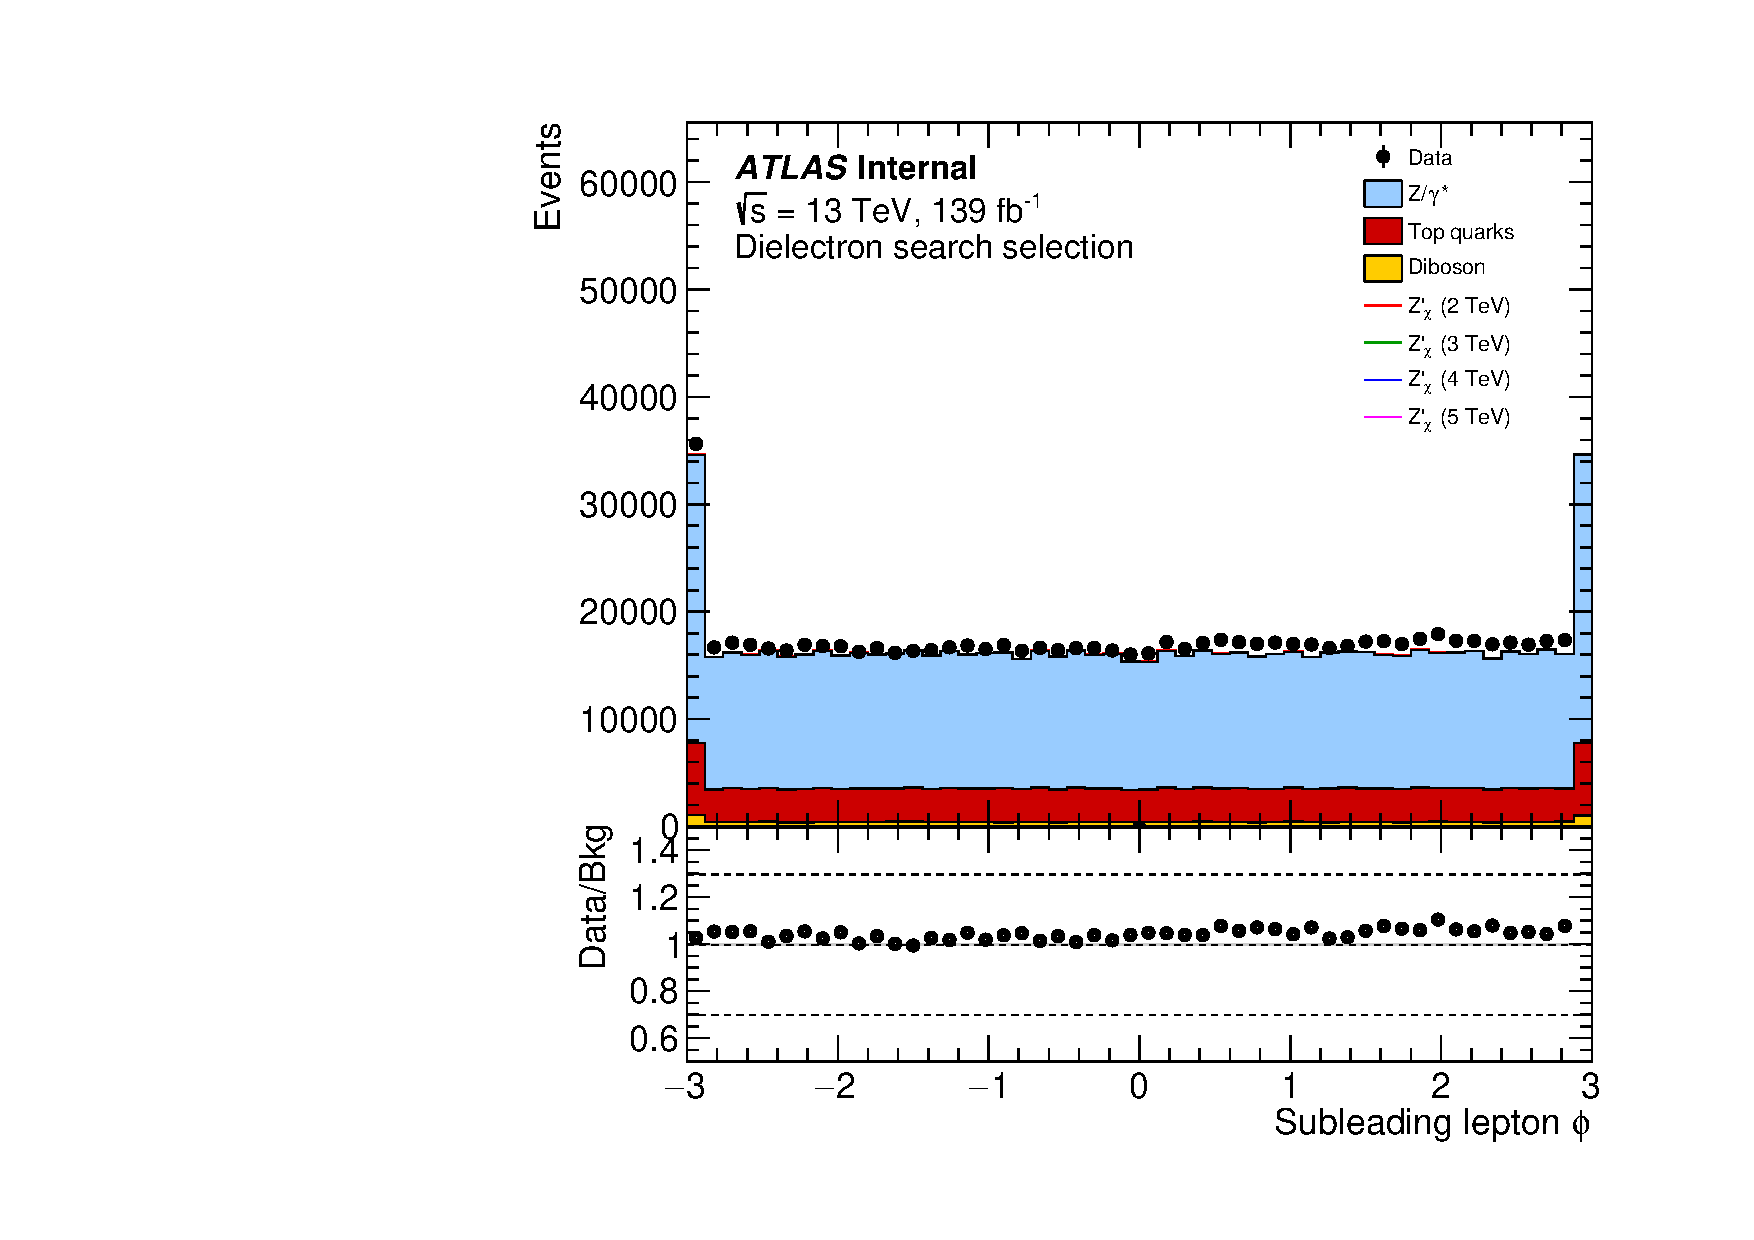
\includegraphics[width=1\textwidth]{figures/ci/dataMc/stacks_mc16e_2015-2018_ee_phi2.pdf}
%     \subcaption{}
% \end{minipage}
% \caption{Kinematic distributions in the $ee$ channel. (a) $E_T^\text{miss}$, (b) dielectron \pt, leading electron $\phi$, and subleading electron $\phi$.}
% \label{fig:}
% \end{figure}
% \clearpage
% }

% \afterpage{
% \begin{figure}[h!]
% \captionsetup[subfigure]{position=b}
% \centering
% \begin{minipage}[b]{.45\linewidth}
%     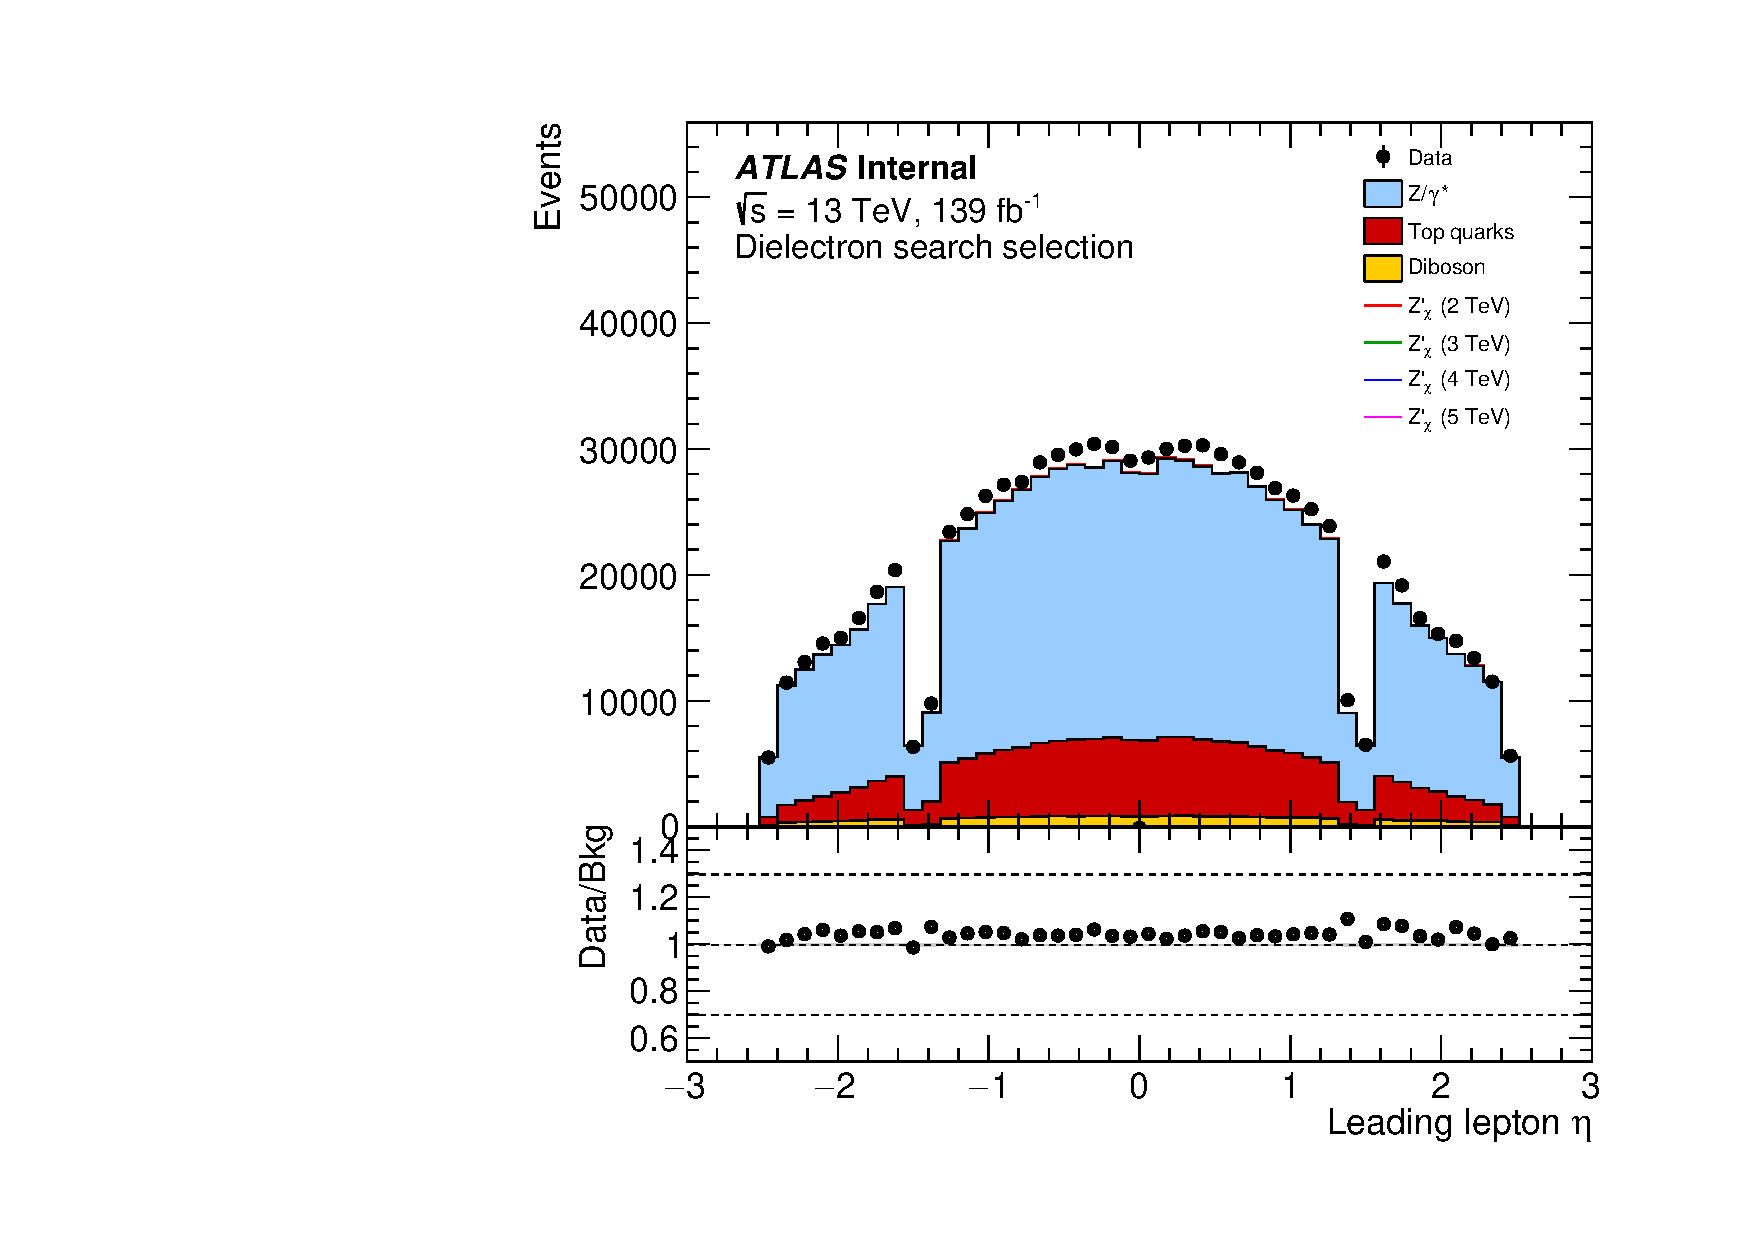
\includegraphics[width=1\textwidth]{figures/ci/dataMc/stacks_mc16e_2015-2018_ee_eta1.pdf}
%     \subcaption{}
% \end{minipage} 
% \begin{minipage}[b]{.45\linewidth}
%     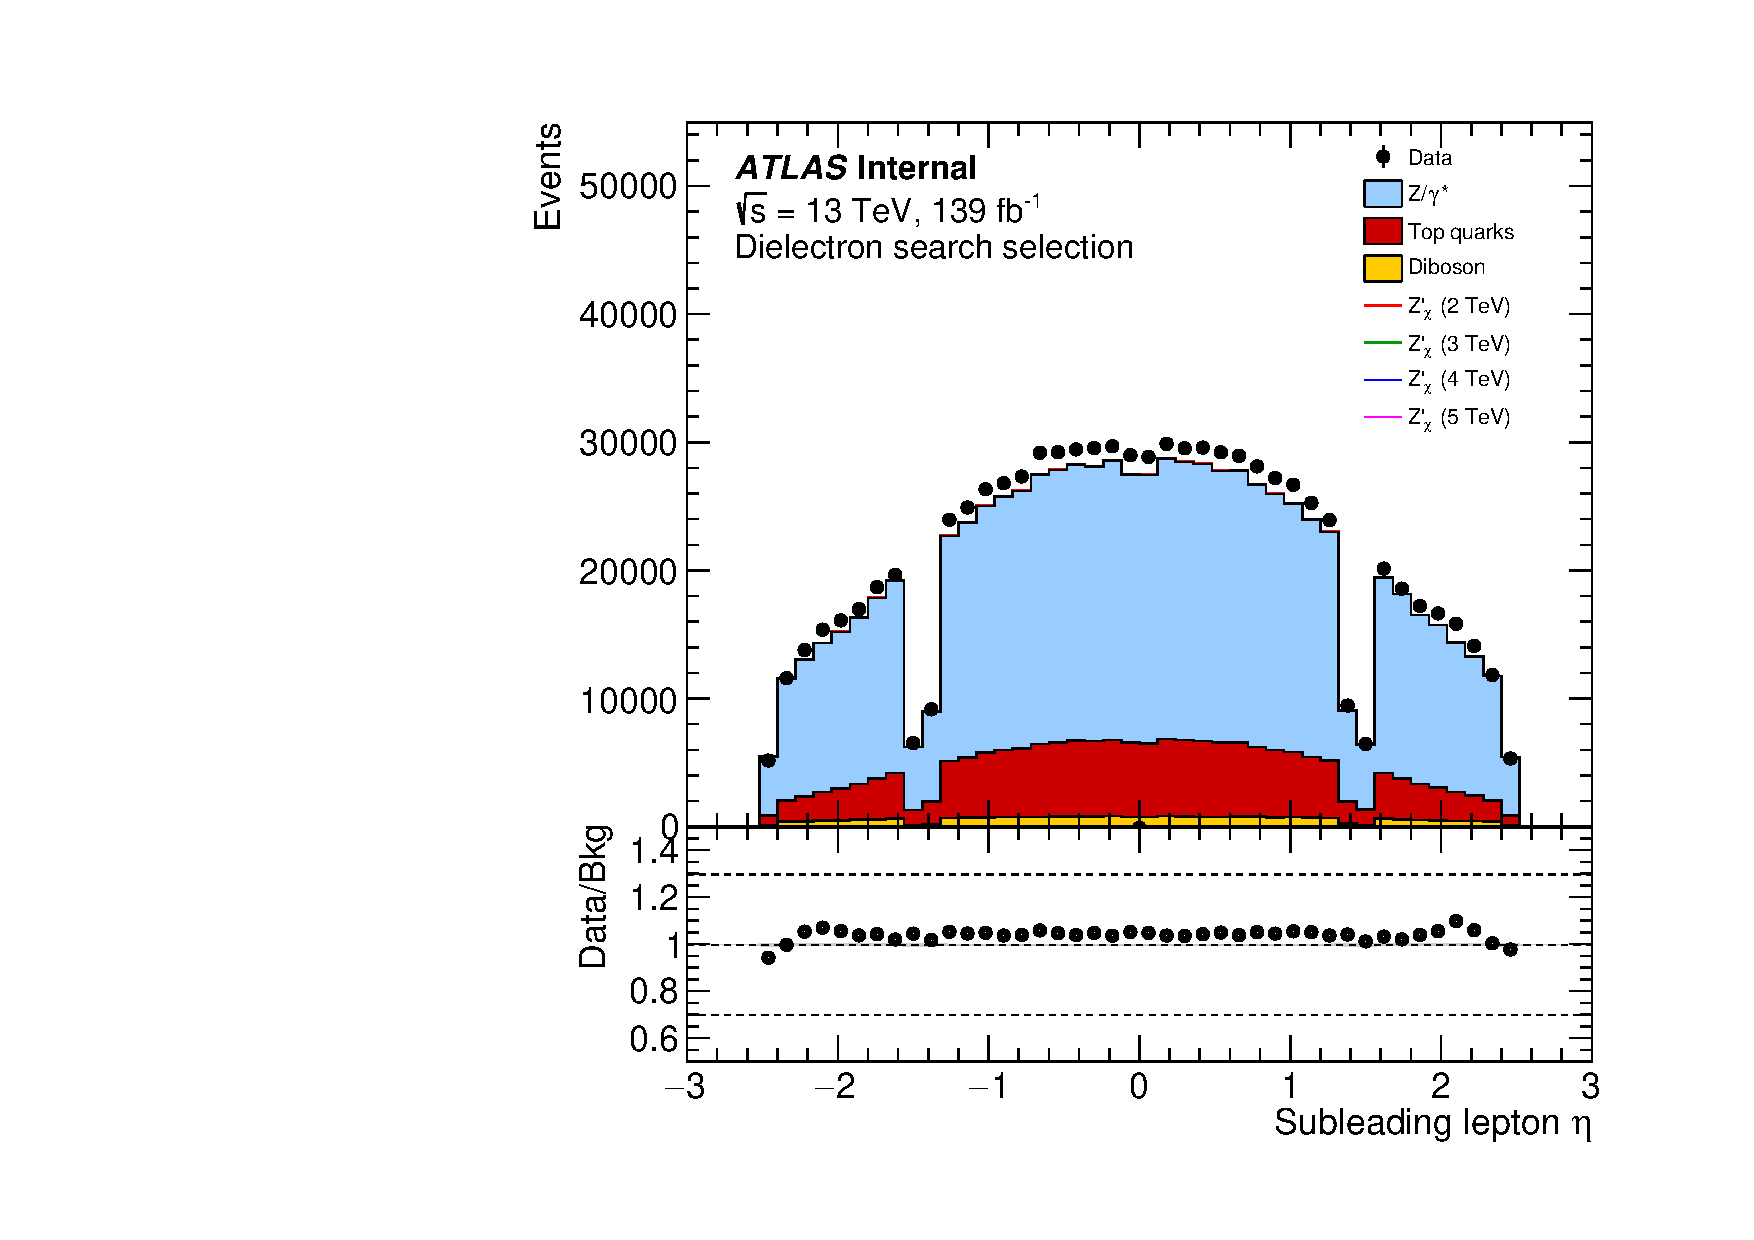
\includegraphics[width=1\textwidth]{figures/ci/dataMc/stacks_mc16e_2015-2018_ee_eta2.pdf}
%     \subcaption{}
% \end{minipage}\\
% \begin{minipage}[b]{.45\linewidth}
%     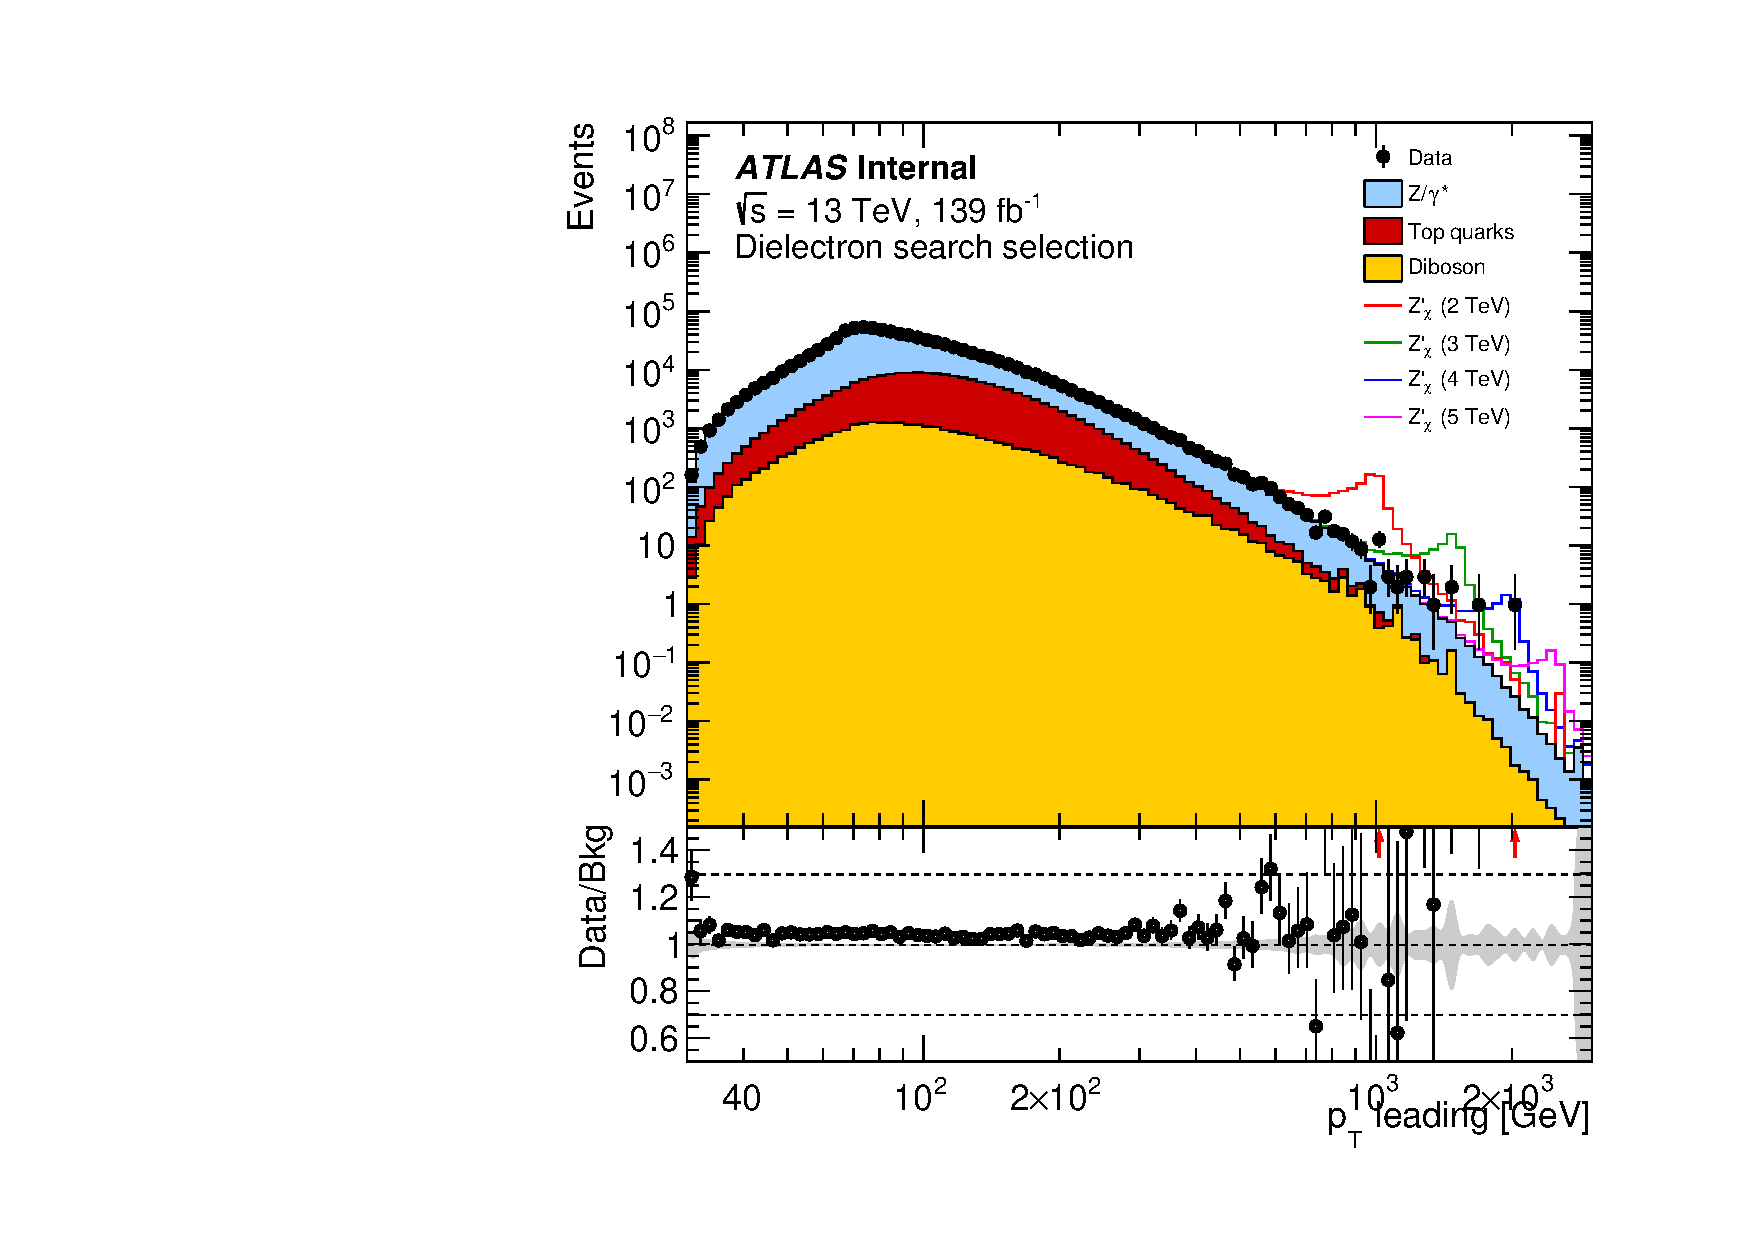
\includegraphics[width=1\textwidth]{figures/ci/dataMc/stacks_mc16e_2015-2018_ee_pt1_log100.pdf}
%     \subcaption{}
% \end{minipage}
% \begin{minipage}[b]{.45\linewidth}
%     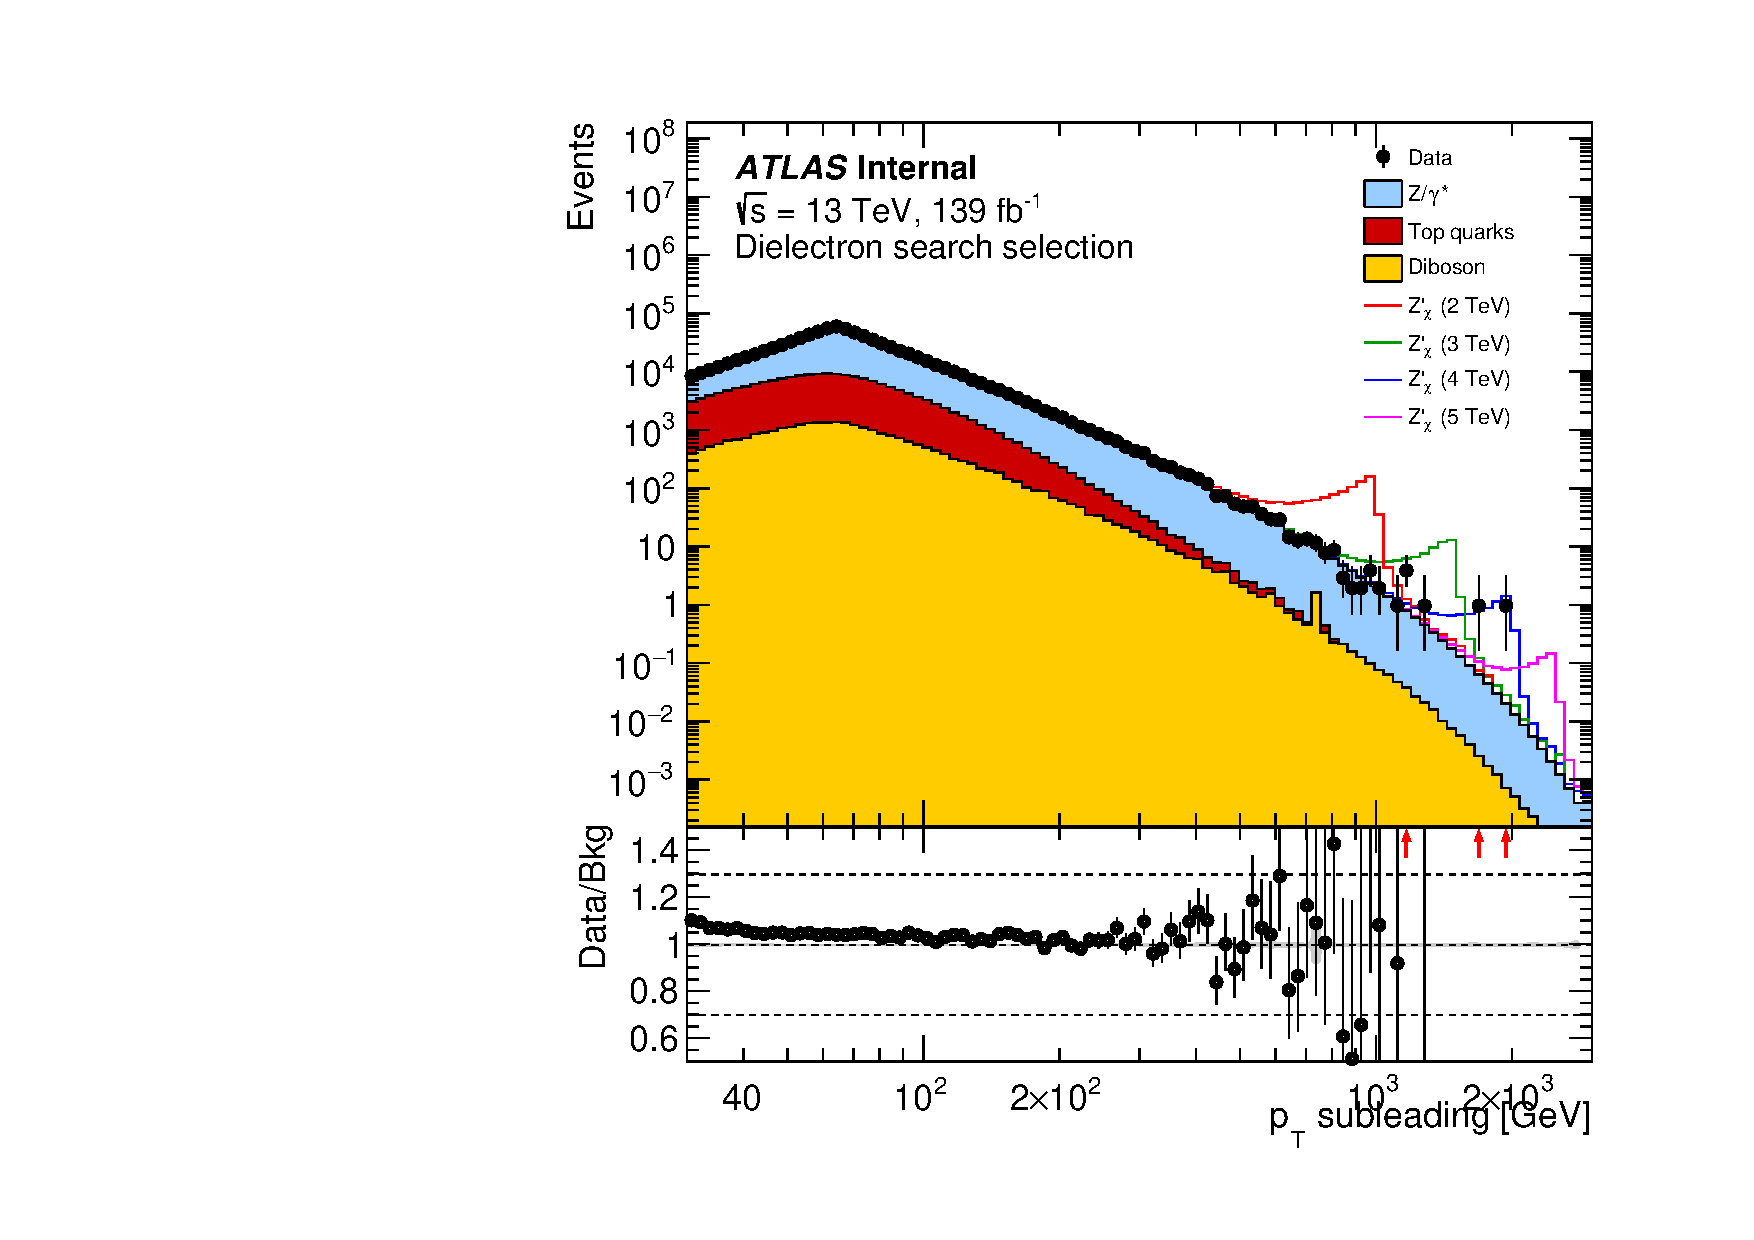
\includegraphics[width=1\textwidth]{figures/ci/dataMc/stacks_mc16e_2015-2018_ee_pt2_log100.pdf}
%     \subcaption{}
% \end{minipage}
% \caption{Kinematic distributions in the $ee$ channel. (a) leading electron $\eta$, (b) subleading electron $\eta$, leading electron \pt, and subleading electron \pt.}
% \label{fig:}
% \end{figure}
% \clearpage
% }

% \afterpage{
% \begin{figure}[h!]
% \captionsetup[subfigure]{position=b}
% \centering
%  \begin{minipage}[b]{.45\linewidth}
%     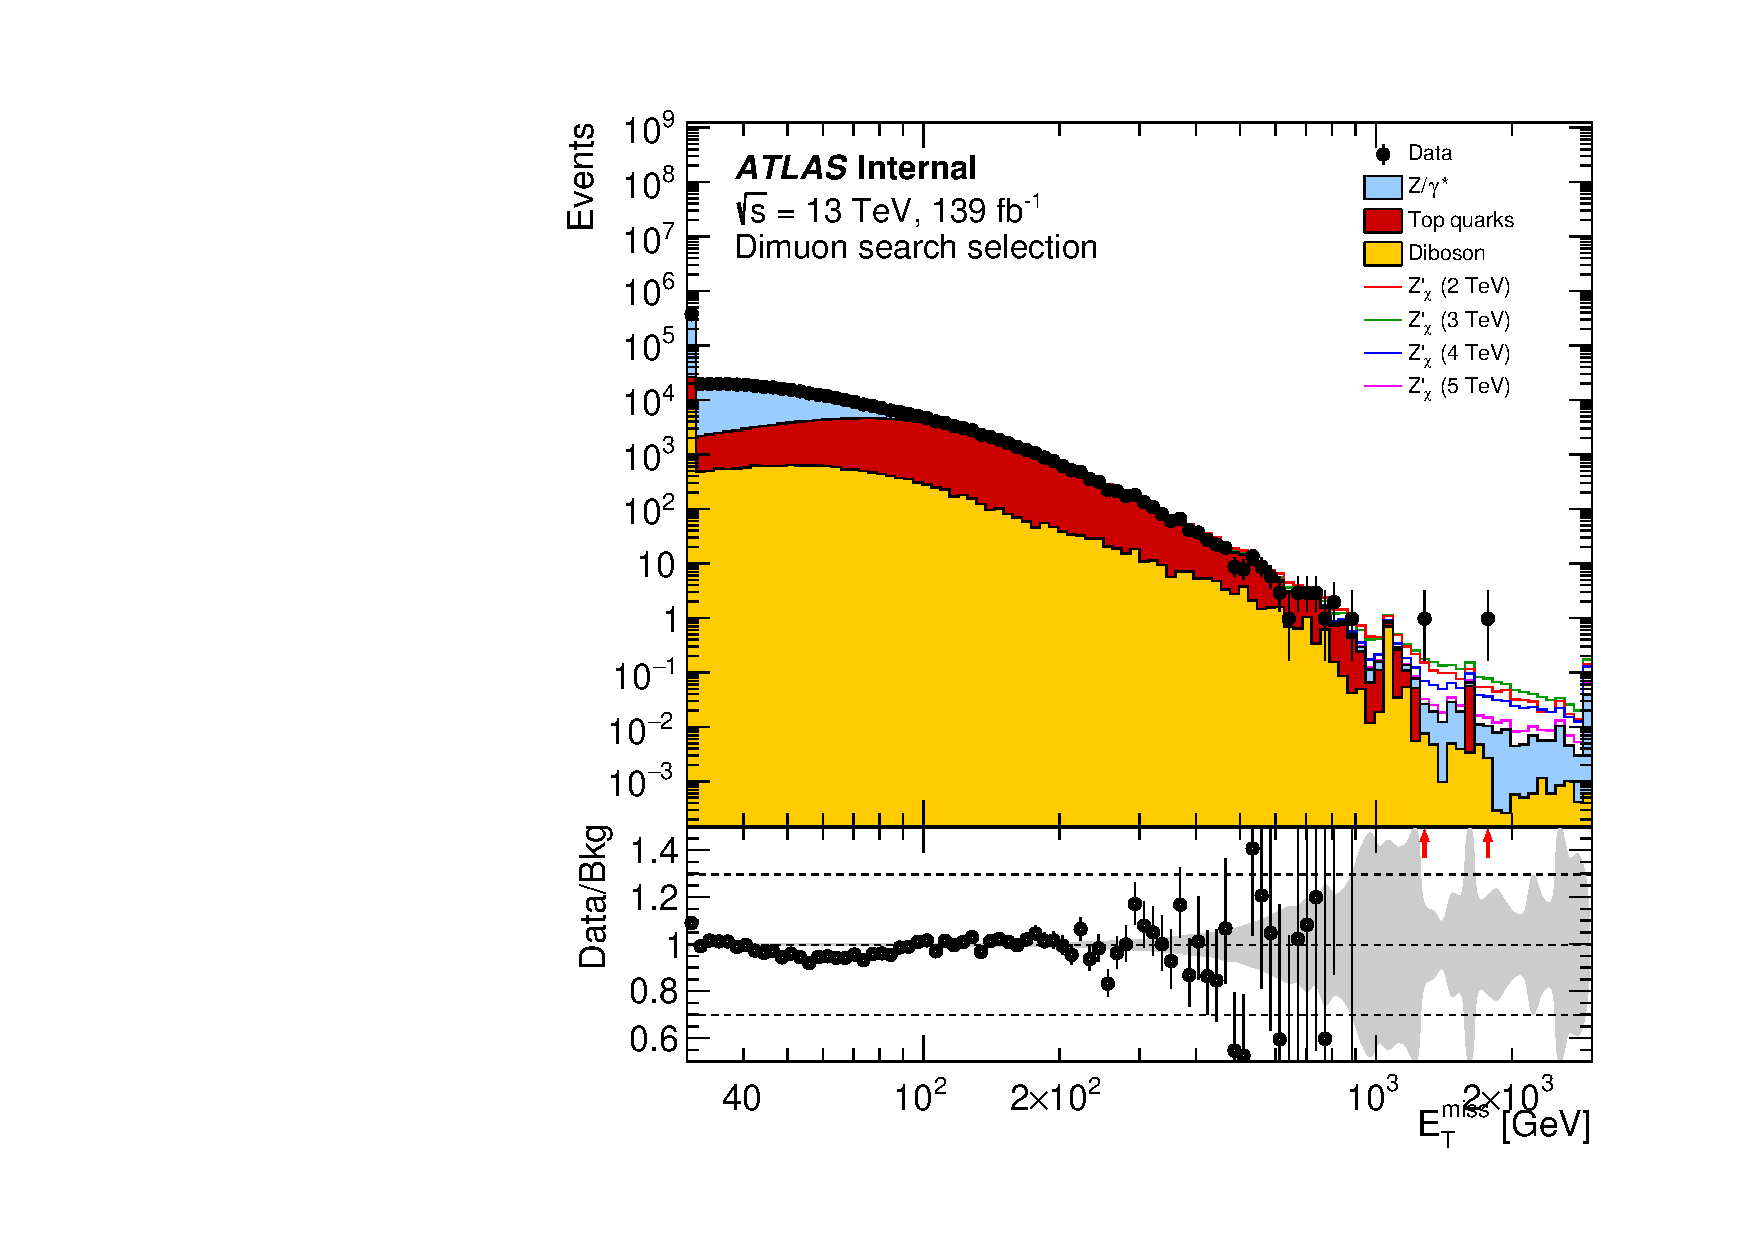
\includegraphics[width=1\textwidth]{figures/ci/dataMc/stacks_mc16e_2015-2018_uu_met_log100.pdf}
%     \subcaption{}\label{fig:1a}
% \end{minipage}
% \begin{minipage}[b]{.45\linewidth}
%     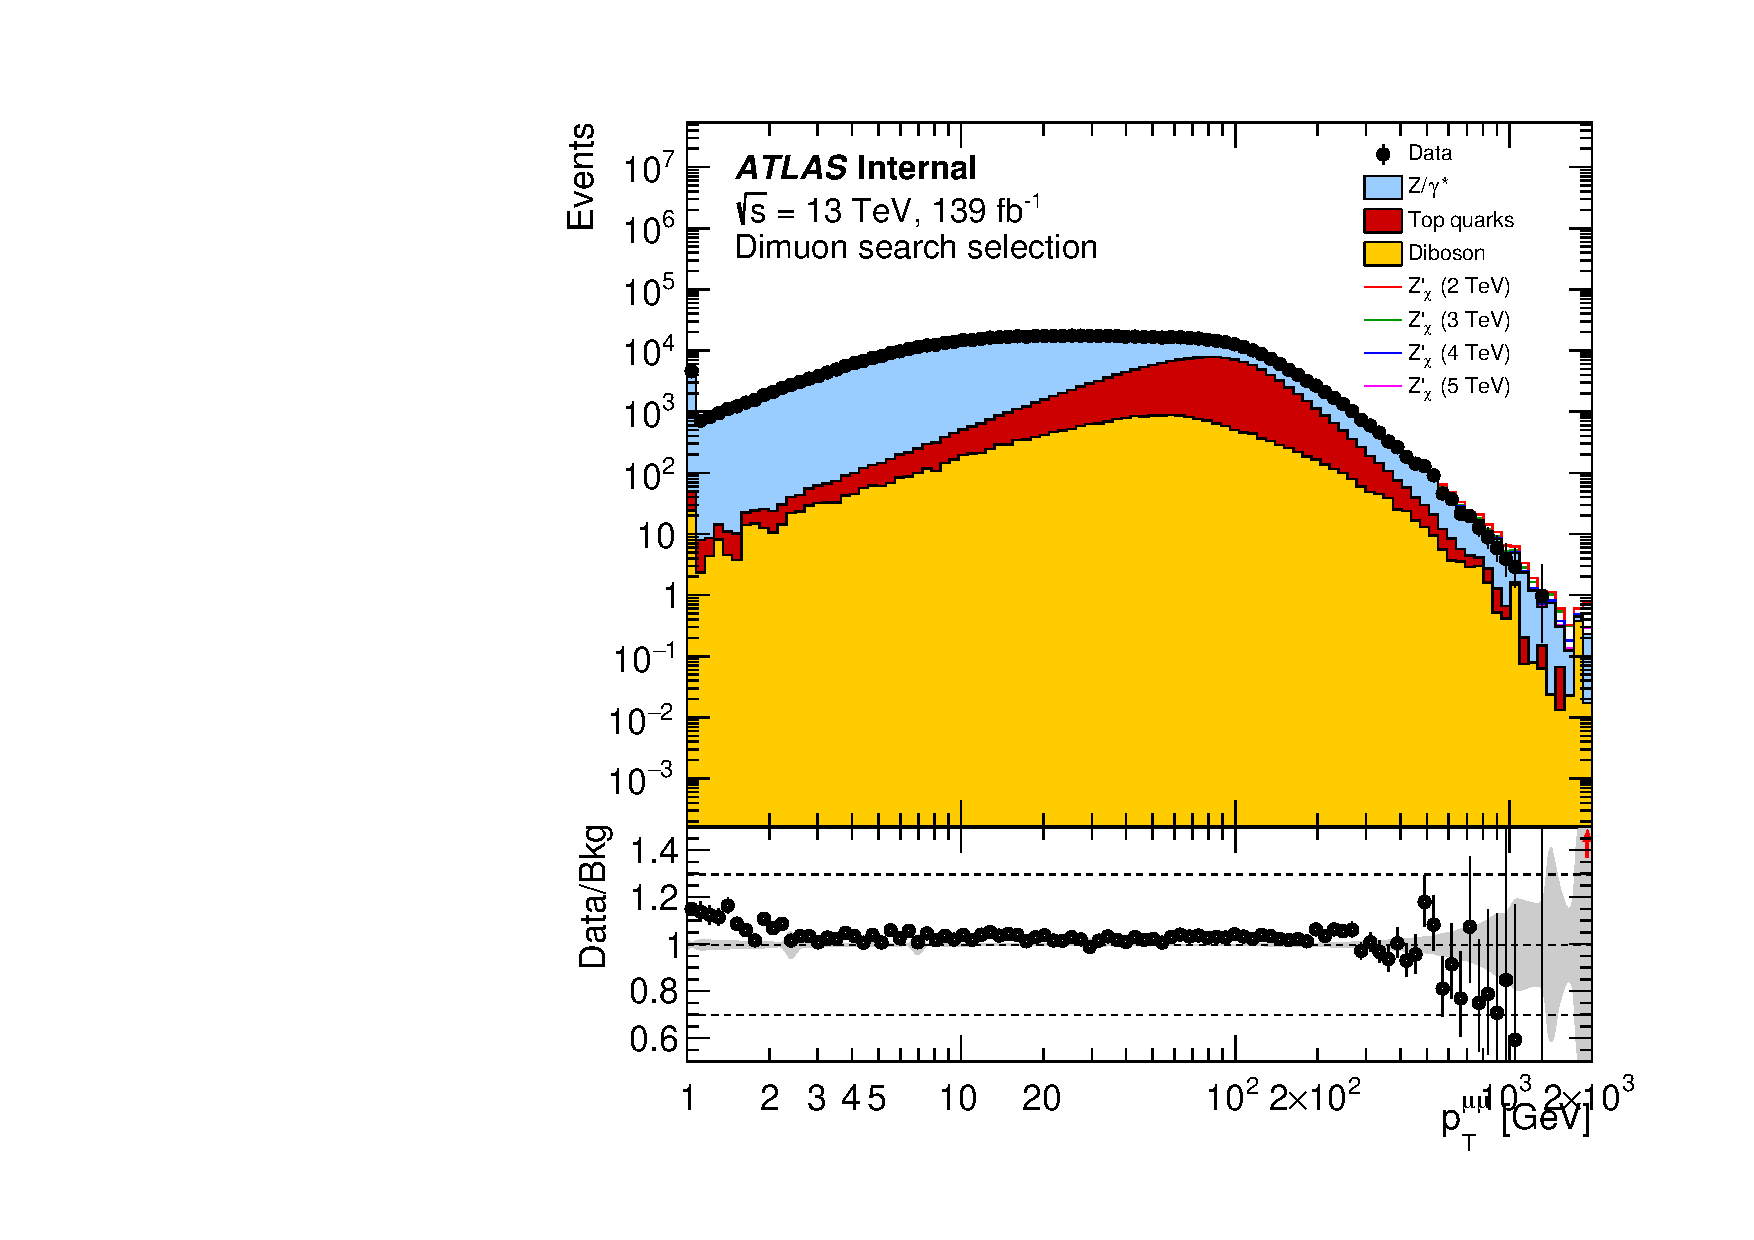
\includegraphics[width=1\textwidth]{figures/ci/dataMc/stacks_mc16e_2015-2018_uu_ptll_log100.pdf}
%     \subcaption{}
% \end{minipage} \\
% \begin{minipage}[b]{.45\linewidth}
%     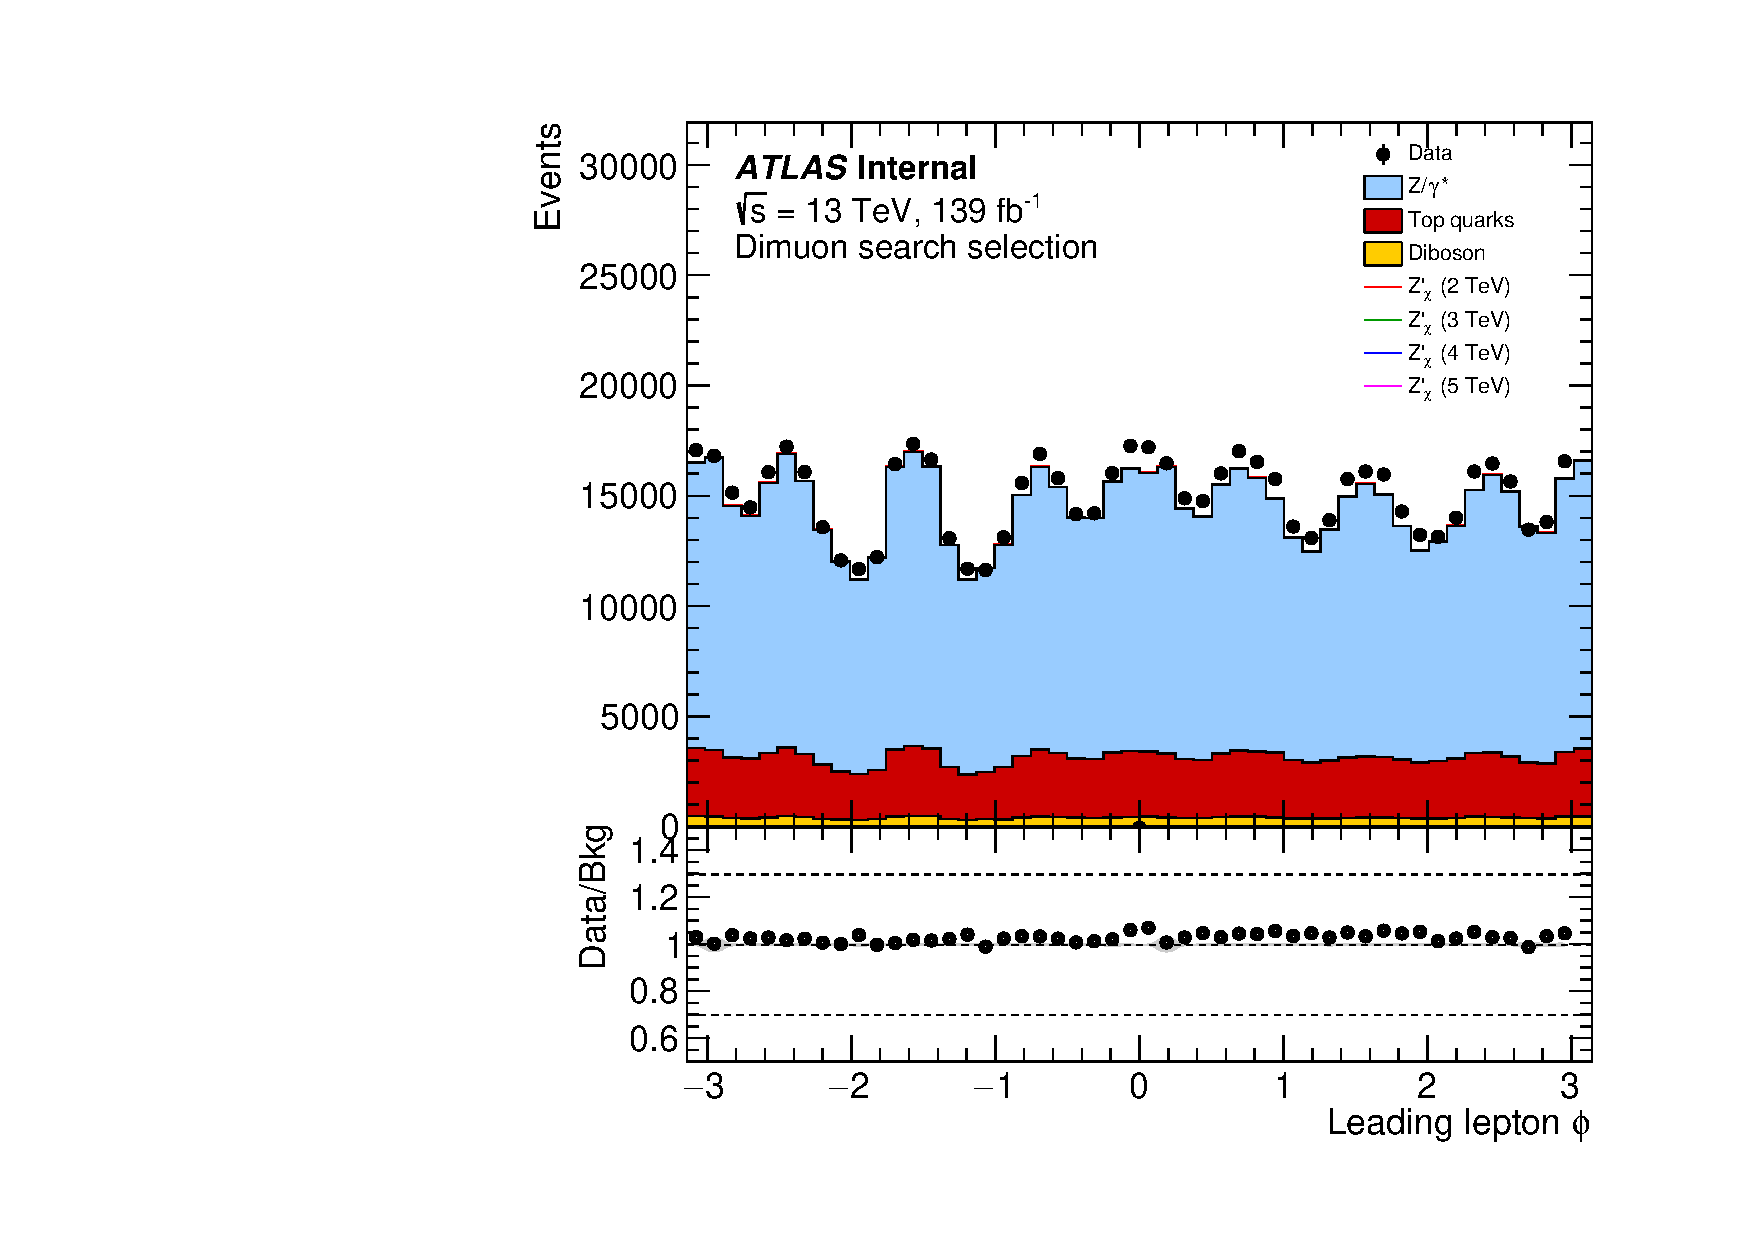
\includegraphics[width=1\textwidth]{figures/ci/dataMc/stacks_mc16e_2015-2018_uu_phi1.pdf}
%     \subcaption{}
% \end{minipage}
% \begin{minipage}[b]{.45\linewidth}
%     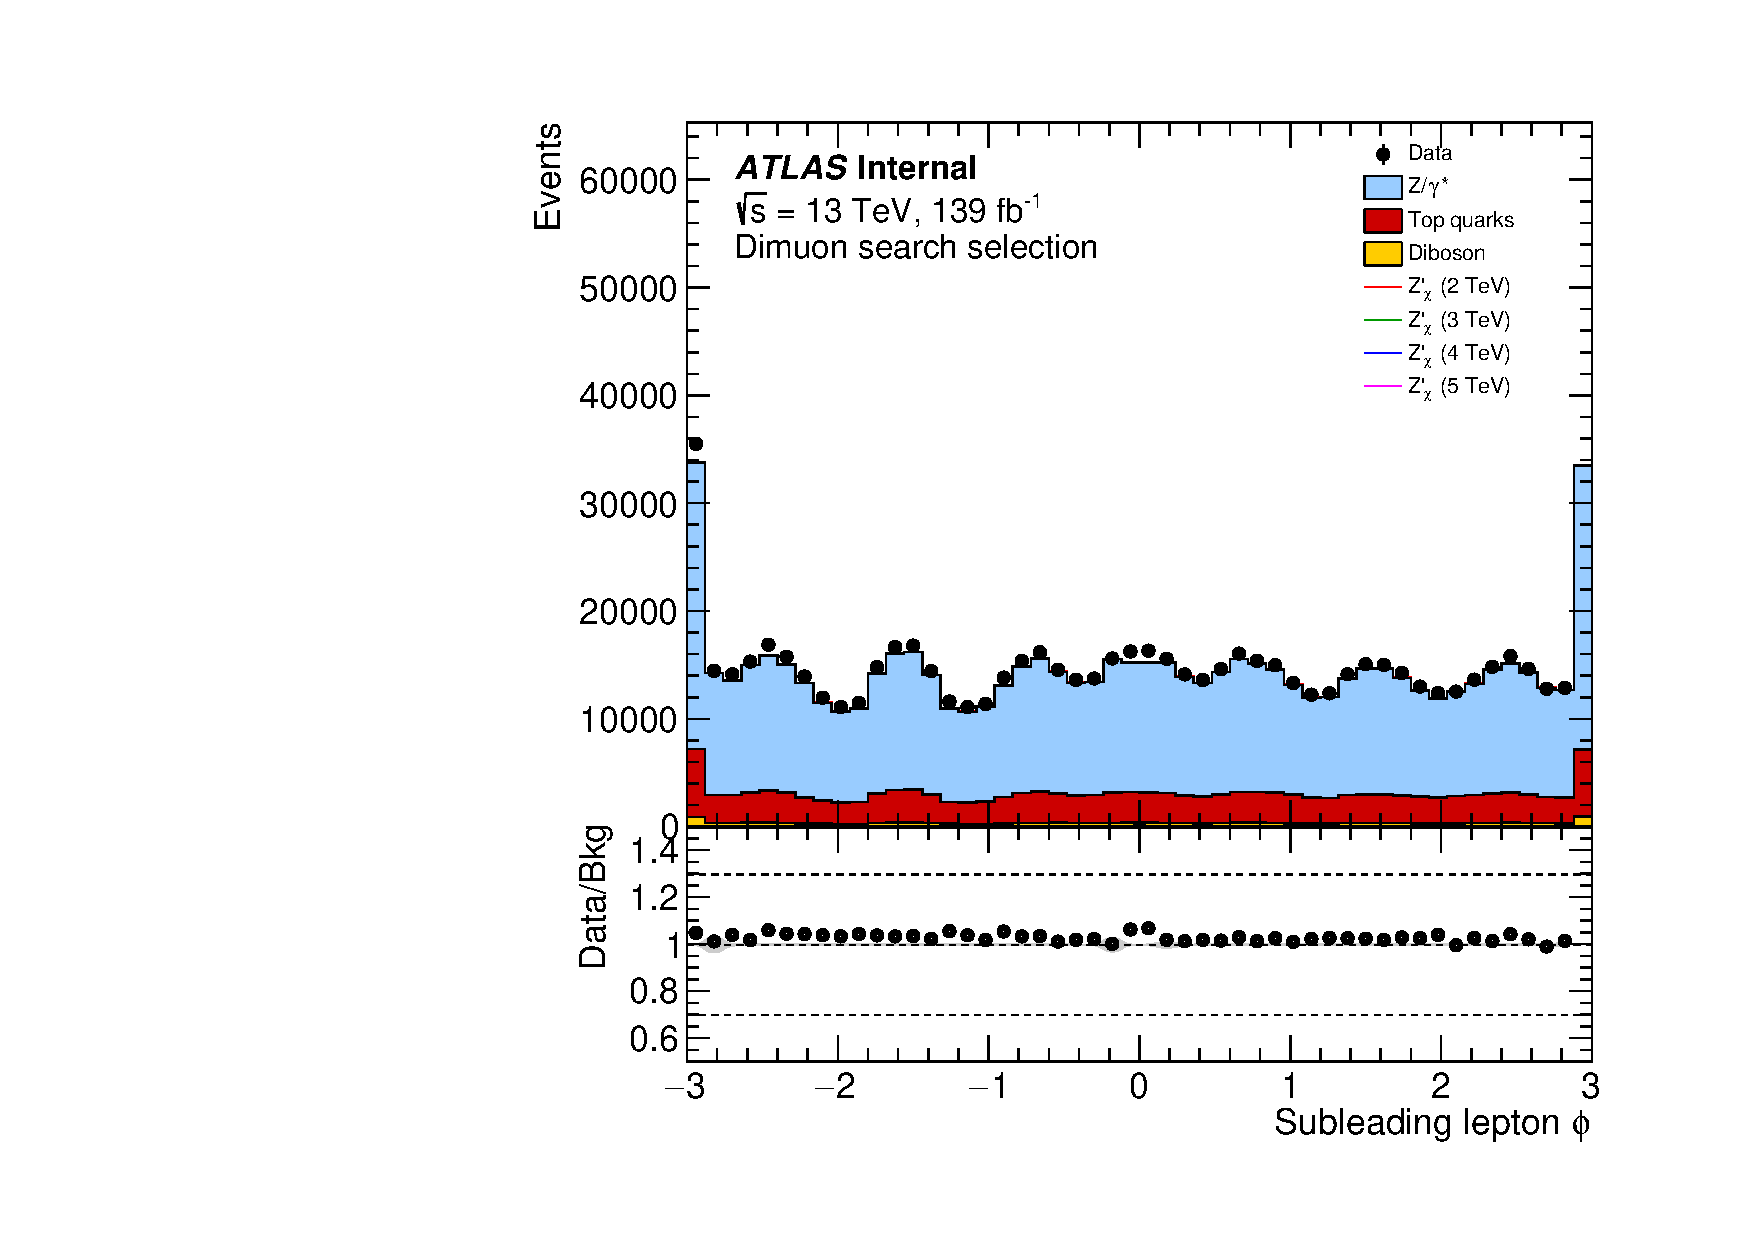
\includegraphics[width=1\textwidth]{figures/ci/dataMc/stacks_mc16e_2015-2018_uu_phi2.pdf}
%     \subcaption{}
% \end{minipage}
% \caption{Kinematic distributions in the $\mu\mu$ channel. (a) $E_T^\text{miss}$, (b) dielectron \pt, leading muon $\phi$, and subleading muon $\phi$.}
% \label{fig:}
% \end{figure}
% \clearpage
% }

% \afterpage{
% \begin{figure}[h!]
% \captionsetup[subfigure]{position=b}
% \centering
% \begin{minipage}[b]{.45\linewidth}
%     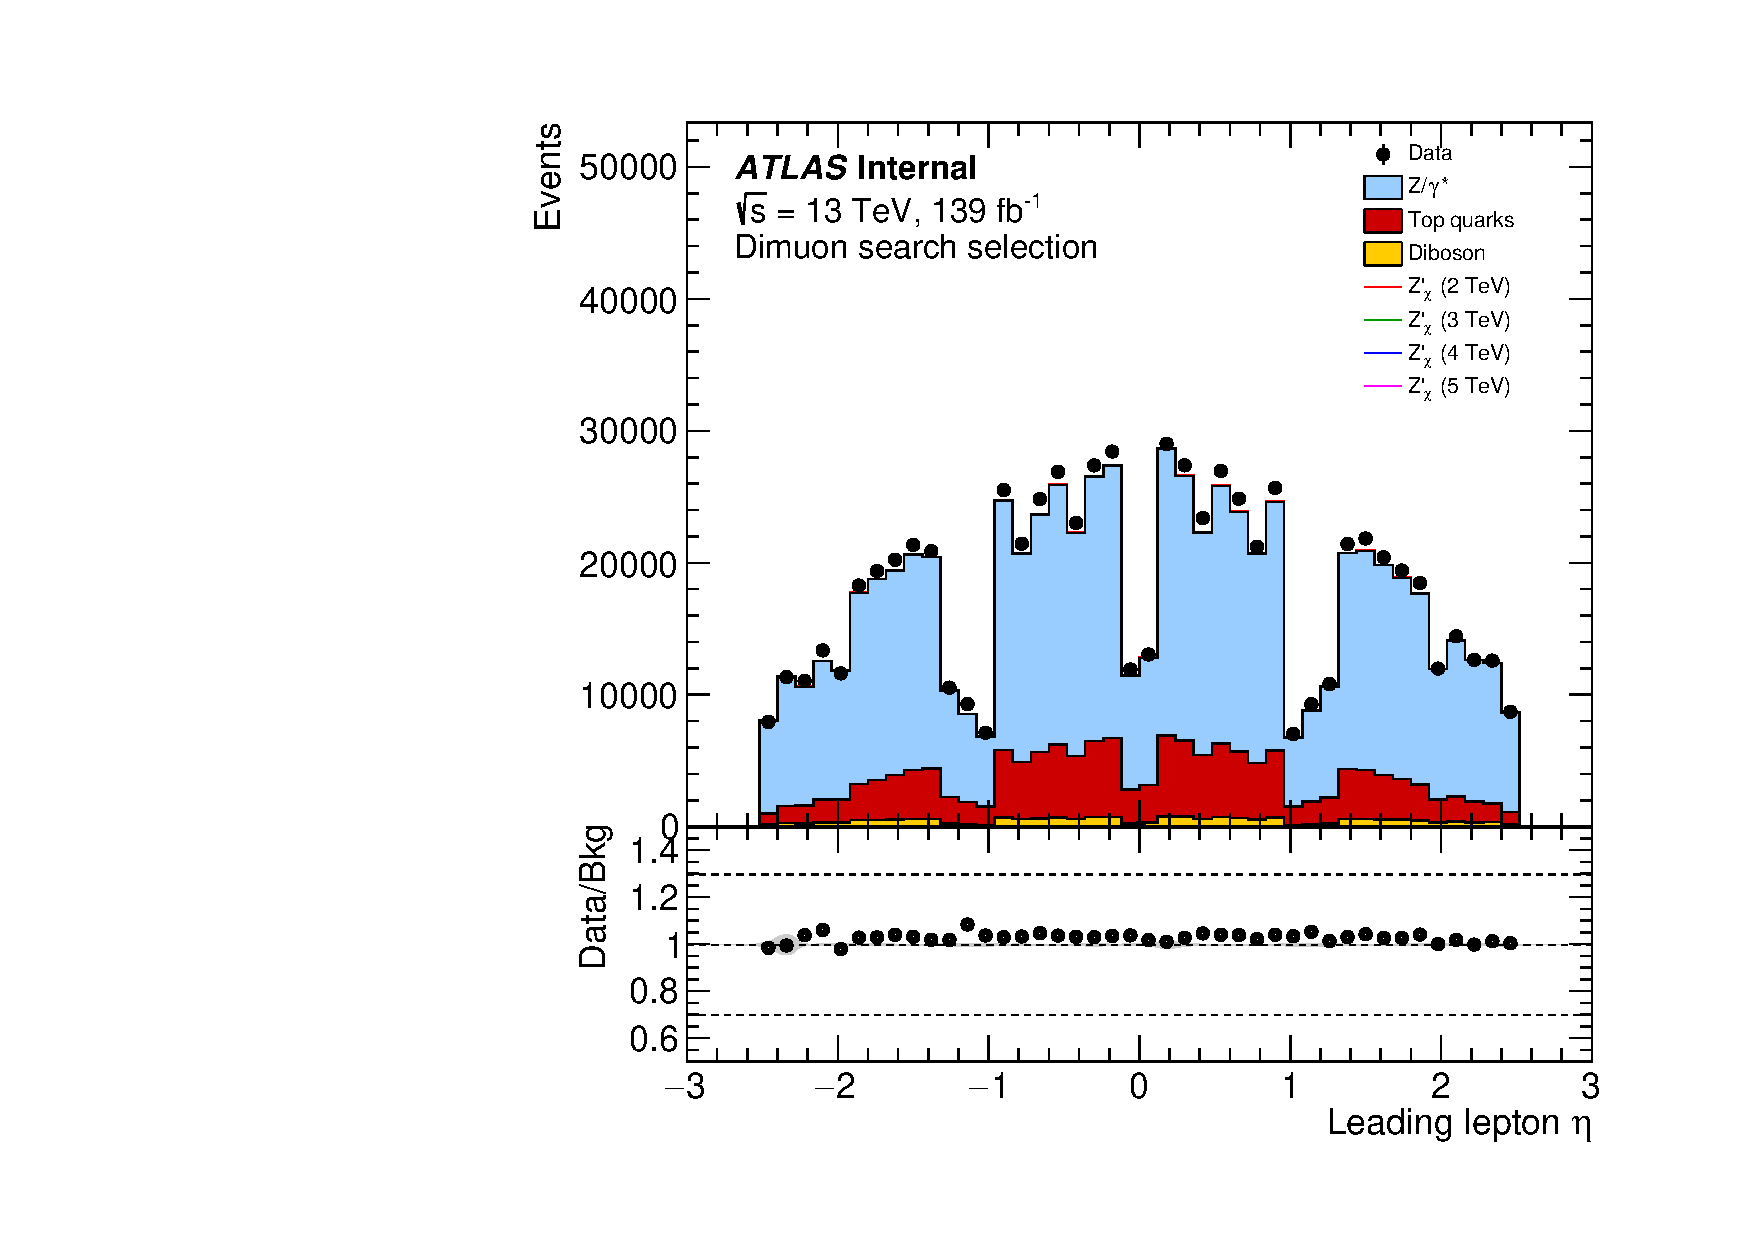
\includegraphics[width=1\textwidth]{figures/ci/dataMc/stacks_mc16e_2015-2018_uu_eta1.pdf}
%     \subcaption{}
% \end{minipage} 
% \begin{minipage}[b]{.45\linewidth}
%     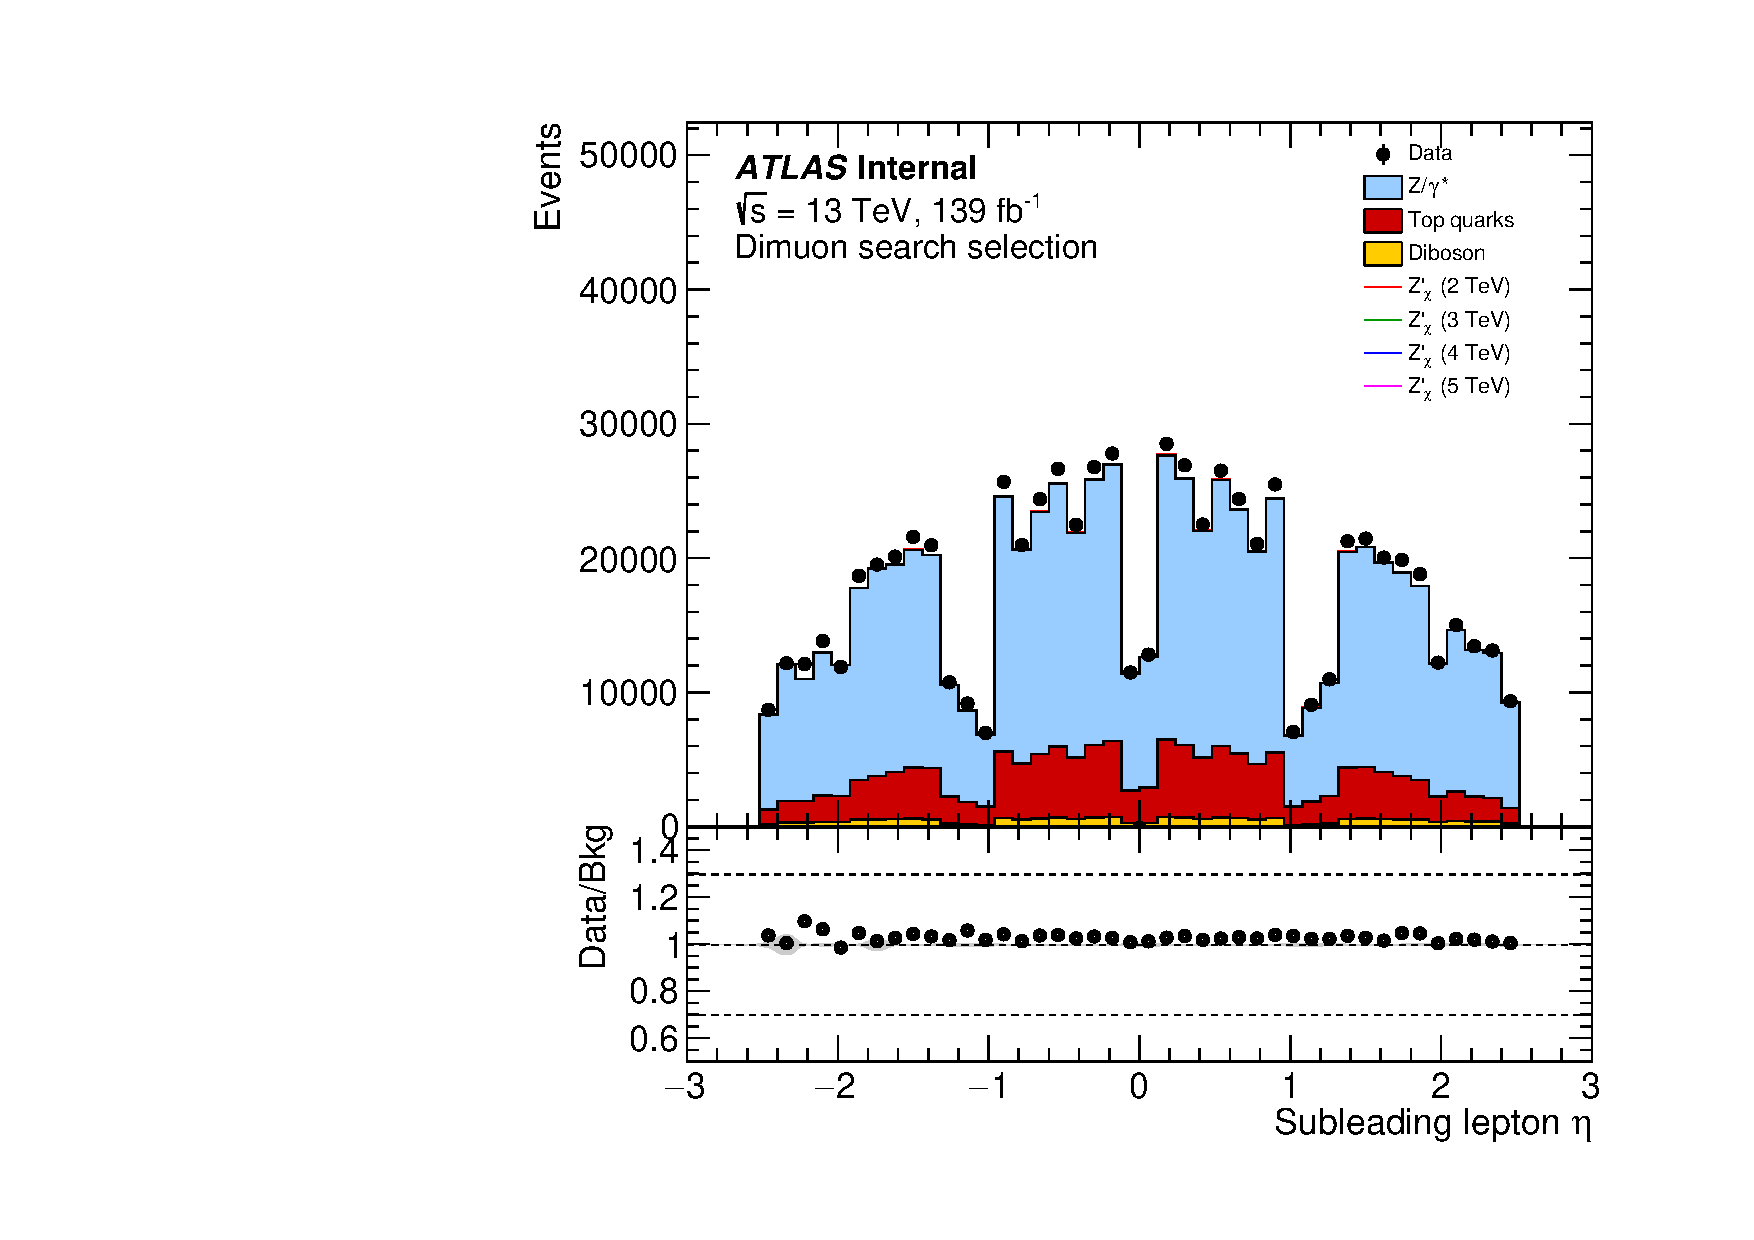
\includegraphics[width=1\textwidth]{figures/ci/dataMc/stacks_mc16e_2015-2018_uu_eta2.pdf}
%     \subcaption{}
% \end{minipage}\\
% \begin{minipage}[b]{.45\linewidth}
%     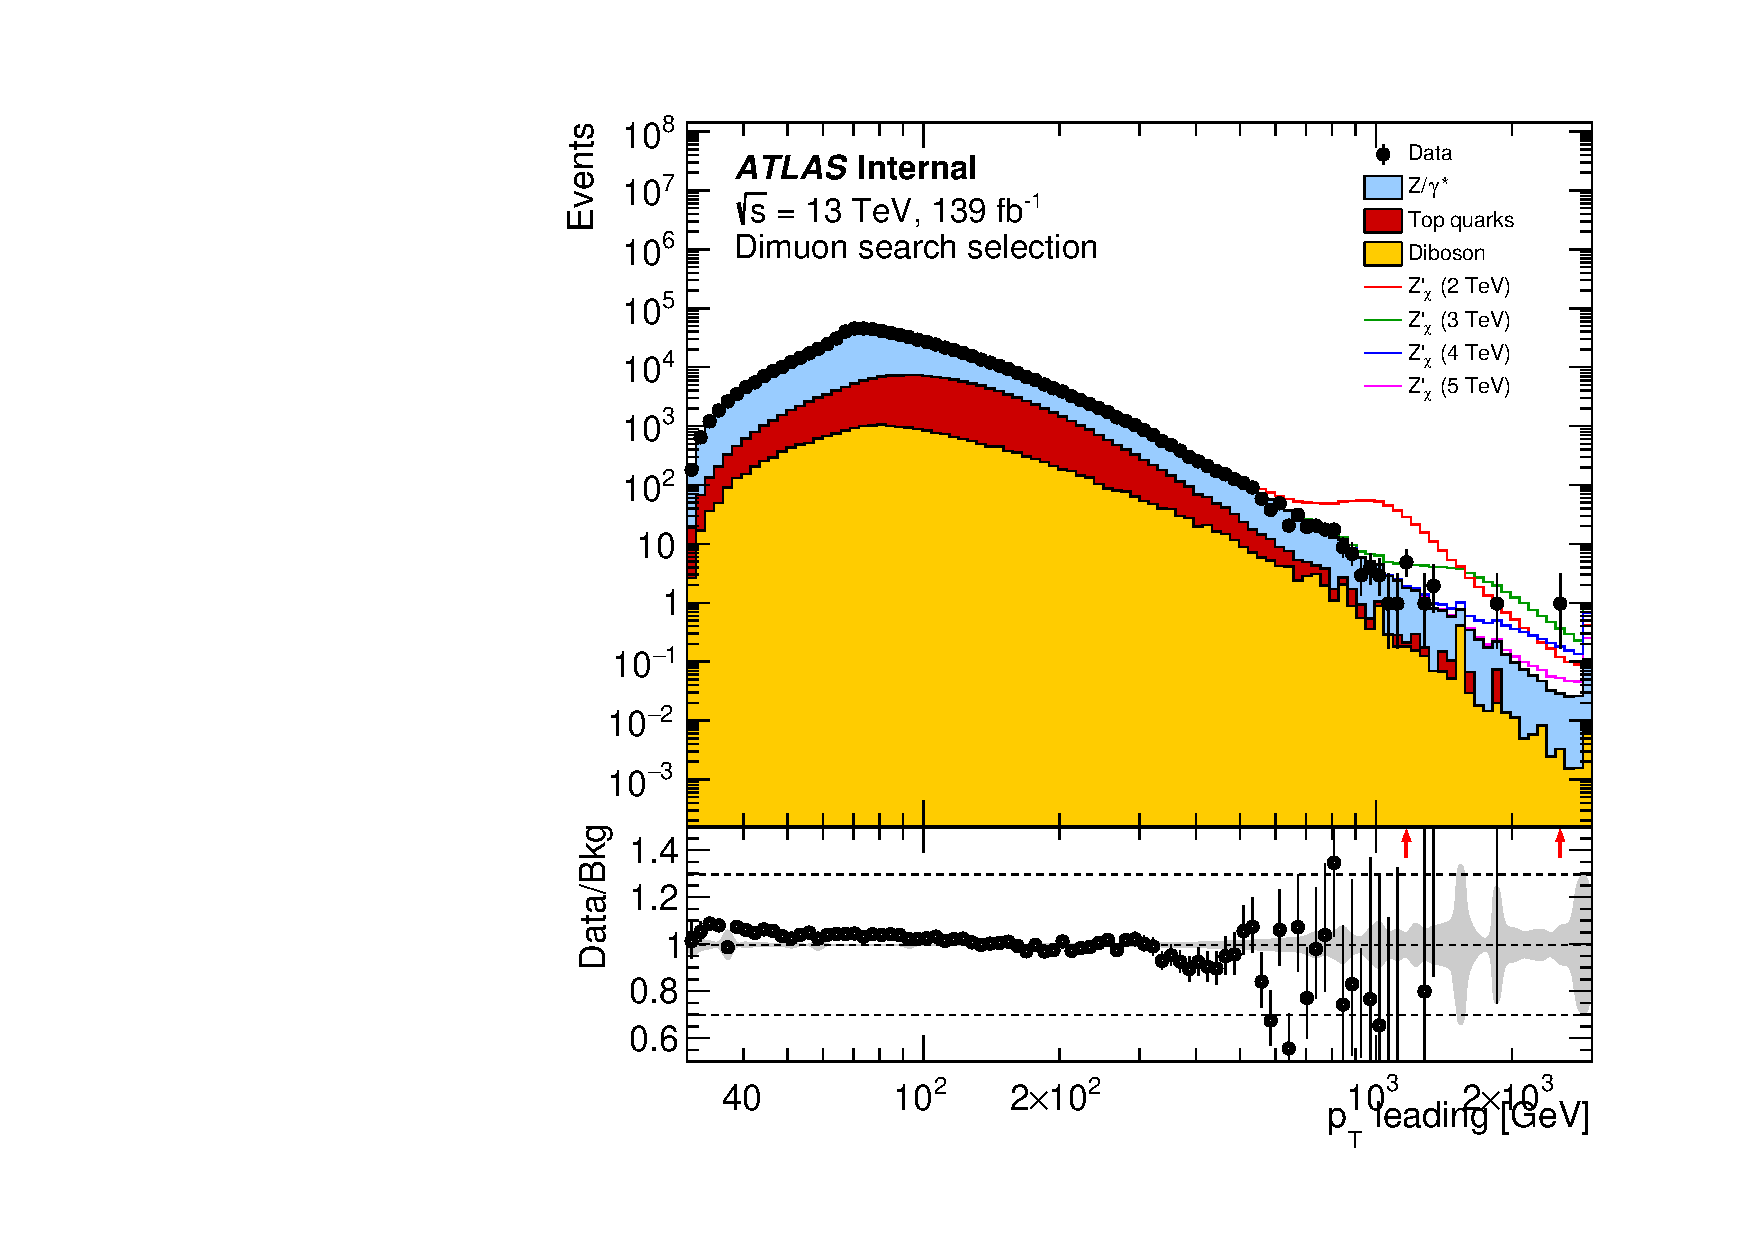
\includegraphics[width=1\textwidth]{figures/ci/dataMc/stacks_mc16e_2015-2018_uu_pt1_log100.pdf}
%     \subcaption{}
% \end{minipage}
% \begin{minipage}[b]{.45\linewidth}
%     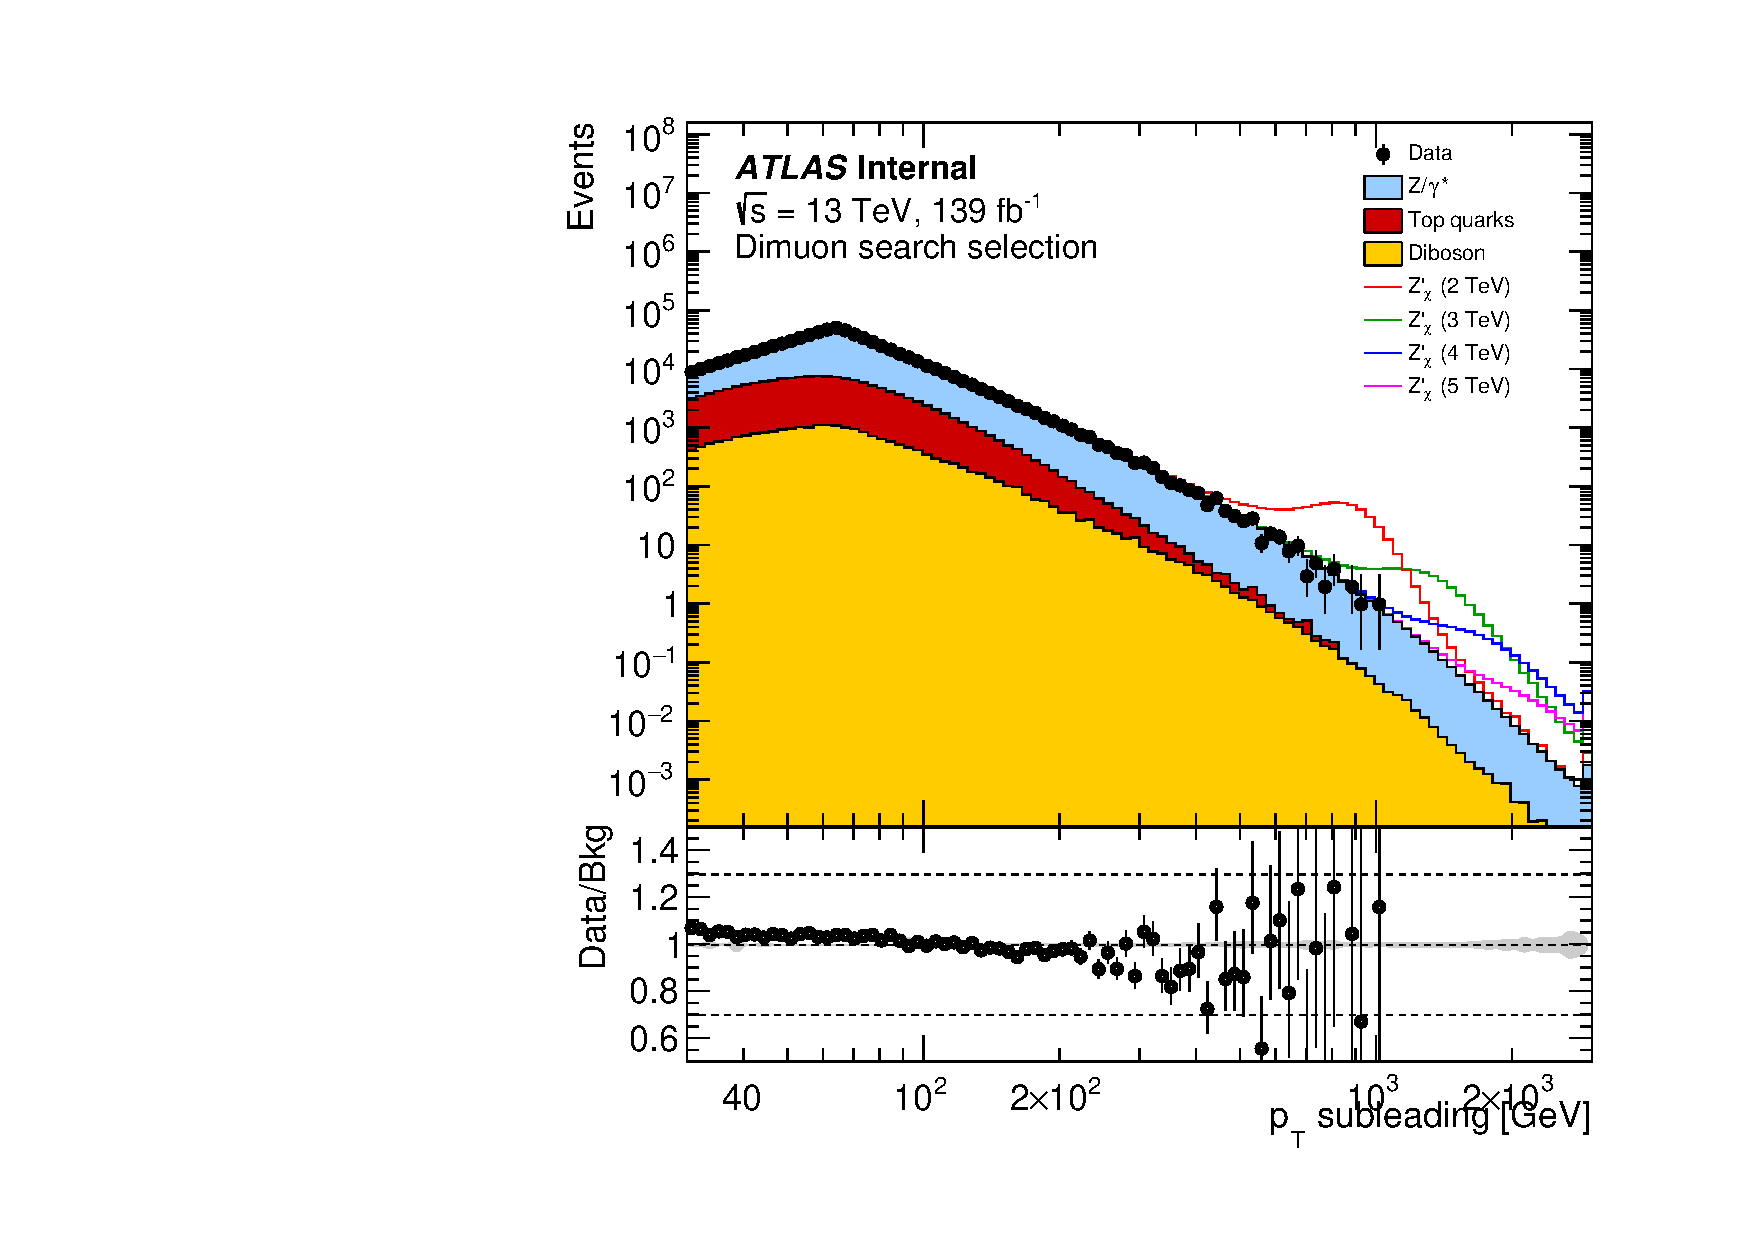
\includegraphics[width=1\textwidth]{figures/ci/dataMc/stacks_mc16e_2015-2018_uu_pt2_log100.pdf}
%     \subcaption{}
% \end{minipage}
% \caption{Kinematic distributions in the $\mu\mu$ channel. (a) leading muon $\eta$, (b) subleading muon $\eta$, leading muon \pt, and subleading electron \pt.}
% \label{fig:}
% \end{figure}
% \clearpage
% }

% \clearpage

\section{Background Modeling}\label{sec:ciBkg}

An expectation of the number of events under the background-only hypothesis is needed for each of the four signal regions.
This raises the question of what exactly is meant by \emph{background}.
In the full mass range, the observed data are considered to have been produced according to some PDF.
If the PDF does not contribute from a signal-like production mechanism, then this is a background-PDF.
This is emphatically not the same thing as the physical truth-PDF that has generated the collected data.
The background-only hypothesis predicts that the event yield in each signal region equals the yield predicted by the background-PDF, normalized to match the integrated luminosity.
Of course, this background-PDF is not explicitly known, and therefore a methodology for estimating it's predicted yield is needed.
This section describes how this is done using an estimate in the CR.

This search uses a functional form fit to the shape of the data in a low mass control region and extrapolated into the high mass signal region, where it is integrated.
In principle, any functional form is acceptable, as long as the uncertainties on the background estimate in the SR are properly measured.
In practice, to produce competitive results, it is necessary to select a functional form that well models the underlying distribution that has generated the background component of the data.

The functional form was chosen from an extensive list of candidates, drawn from similar studies, for its stability during extrapolations and the ability to model the simulated background. Here, stability refers to the function not to tend to behave nonphysically.
The procedure to determine the functional form of the background is as follows.
The smooth functional form used to model the background is chosen from about 50 candidate functions.
Each function is fit to the dilepton mass background template, consisting of the sum of all the simulated background contributions, in a variety of CRs, and extrapolated to the respective SRs.
The data and simulation are both fit using a binned-likelihood maximization with a bin width of 1~GeV.
The distribution of the pulls, defined as (fit--simulation)/fit for each bin, is obtained for each potential configuration of CR and SR.
A function that results in pulls below three across all the ranges considered (CRs and SRs) is marked as acceptable.
This requirement is particularly important in the SRs to veto functions that exhibit unphysical behavior at the tail.
Additionally, it is important to ensure a good description of the simulated background template in the CRs.
Out of about 50 initial functions, five are found to satisfy this requirement equally well.
The residual mis-modeling by the selected function is measured later and taken as an uncertainty.
The functions that were found to best satisfy these criteria are given in Equations \ref{eqn:ciBkgEe} and \ref{eqn:ciBkgMm} for $ee$ and $\mu\mu$ channels respectively.

\begin{equation}\begin{split} \label{eqn:ciBkgEe}
f_\textrm{b}(\mee) &= f_{\mathrm{BW},Z}(\mee) \cdot \left(1 - x\right)^{b} \cdot x^{\sum_{i=0}^3 p_i\log(x)^i} \\
\end{split}\end{equation} 

\begin{equation}\begin{split}\label{eqn:ciBkgMm}
f_\textrm{b}(\mee) &= f_{\mathrm{BW},Z}(\mee) \cdot \left(1 - x^{1/3}\right)^{b} \cdot x^{\sum_{i=0}^3 p_i\log(x)^i} \\
\end{split}\end{equation} 

Here, $x = m_{\ell\ell}/\sqrt{s}$.
The first term, $f_{\mathrm{BW},Z}(m_{\ell\ell})$, is a non-relativistic Breit--Wigner function with $m_Z = 91.1876$~GeV and $\Gamma_Z = 2.4952$~GeV.
This primarily dictates the function shape in the low-mass regime of the control region.
The second term, $(1-x^{c})^{b}$, shapes the high-mass behavior of the function by ensuring that the background shape evaluates to zero at $x\to 1$.
The parameter $b$ is fixed to values obtained from fits to the simulated background.
In the third term, the parameters $p_i$ with $i=0,..,3$ are left free in the fits.
The function $f_\textrm{b}(m_{\ell\ell})$ is treated as a probability density function in the fits performed in the CR.
This function is then normalized in the CR to $N_\textrm{CR}$, the number of events in the CR in data (or simulation where applicable), where it is assumed that the CR is completely dominated by background events.

The fits are performed using a binned likelihood maximization using the MINUIT algorithm \cite{minuit}.
The functional forms of Equations \ref{eqn:ciBkgEe} and \ref{eqn:ciBkgMm} are fit to a \emph{template}, which may is a histogram filled by either data or simulated data.
In this process, the total log-likelihood of the template is calculated as the sum of the log-likelihood of each template bin to have been generated by the functional form.
Then, each of the flexible parameters of the functional forms is adjusted with MINUIT until the total log-likelihood has reached a maximum.
The functional form with these parameter fitted values is the function with the highest likelihood to generate the observed data.

% Definitions of function vs ''background model''
It is worth explicating some nomenclature. 
The normalized and fitted functions of Equations \ref{eqn:ciBkgEe} and \ref{eqn:ciBkgMm} describe well the differential shape of the data in each CR.
To a lesser extent, these forms also describe the differential shape of the data in each SR.
The background estimate that is used for the purpose of this analysis, however, is the integral of these functions in the SR.

This number is interpreted as the mean number of events to expect in the SR under the background-only hypothesis.
This differs from the true prediction of that hypothesis on three counts.
First, the assumption of particular forms of Equations \ref{eqn:ciBkgEe} and \ref{eqn:ciBkgMm} implicitly assumes these match the shape of the background-PDF.
Second, the fits are performed to the finite data in the CR, not to the underlying PDF.
This means that statistical fluctuations in the CR influence the shape of the fitted function, and therefore background estimate.
Third, the fit performed in the CR is data generated by the truth-PDF, not the background-PDF. 
This implicitly assumes that no signal process contributes to the events in the CR. 
These three assumptions mean that the background estimate described here is, in fact, an approximation of the true underlying background yield in each SR.
The accuracy of this approximation is described by systematic uncertainties on the background estimate.

\section{Signal Modeling}\label{sec:ciSig}

Although the results of this search can be interpreted for multiple signal models, the model of most interest is that of the \llqq contact interactions.
Contact interactions are described by the Lagrangian in Equation \ref{eqn:ciLagrangian}.
There are five free parameters: the characteristic energy scale \lam, and the parameters $\eta_\text{LL}$, $\eta_\text{RR}$, $\eta_\text{LR}$, and $\eta_\text{RL}$.
The model is simplified by selecting one $\eta_{ij}=\pm1$ for $i,j\in[\text{L,R}]$, and setting the rest as zero.
This describes a model where only one chiral coupling is present, dubbed ``$ij$''.
Furthermore, if $\eta_{ij}=-1$ then the interference of the coupling with the Standard Model is constructive, while if $\eta_{ij}=+1$, it is destructive.
Therefore, eight signal models are considered: four chiral combinations, times two interference patterns, as shown in the table below.
\begin{center}
\begin{tabular}{l l l}
  \toprule
  Lepton channel & Interference & Chirality \\
  \midrule
  $ee$ & Constructive & LL, RL, LR, RR \\
  $ee$ & Destructive & LL, RL, LR, RR \\
  $\mu\mu$ & Constructive & LL, RL, LR, RR \\
  $\mu\mu$ & Destructive & LL, RL, LR, RR \\
  \bottomrule
\end{tabular}
\end{center}


% Generating the TH1 histograms
Signal shapes for the full \mll distribution are modeled using a matrix-element reweighting~\cite{EXOT-2016-05} of the leading-order (LO) DY samples.
This reweighting includes the full interference between the non-resonant signal and the background DY process.
The weight function is the ratio of the analytical matrix-elements of the full CI (including the DY component) and the DY process only, both at LO.
It takes as an input the generated dilepton mass at Born level before FSR, the incoming quarks' flavor and the CI model parameters (\lam, chirality states, and the interference structure).
These weights are applied to the LO DY events to transform these into the CI signal shapes, in steps of $2$~TeV between $\Lambda=12$~TeV and $\Lambda=100$~TeV.
Dilepton mass-dependent higher-order QCD production corrections for the signals are computed with the same methodology as for the DY background, correcting from LO to NNLO.
Similarly, electroweak corrections for the signals are applied in the CI reweighting along with the interference effects, correcting from LO to NLO.
% The ratios of the CI reweighted \mll distributions to the nominal \mll shape are shown for LL chirality in Figure \ref{fig:ciSignalRatiosToNominal}.
The CI component of the signal shape (direct production and interference) is referred to as the \emph{signal}. This is produced by subtracting the LO DY shape from the combined DY+CI shape.
The full \mll signal shapes are shown along with the background function in Figure \ref{fig:ciSignalShape}.

\afterpage{
\begin{figure}[hb]
\begin{center}
\subfloat[][]{{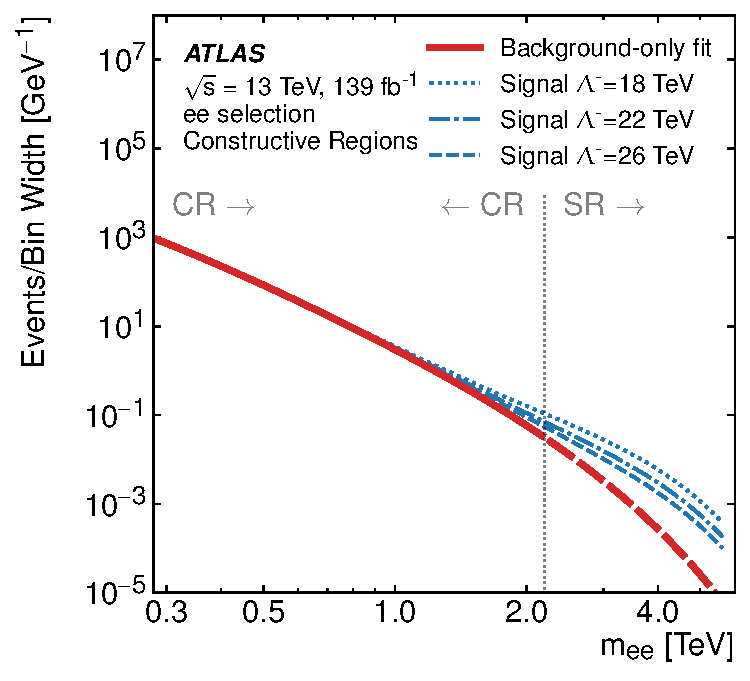
\includegraphics[width=0.45\textwidth]{figures/ci/sigRatio/figaux_01a.pdf}}}
\subfloat[][]{{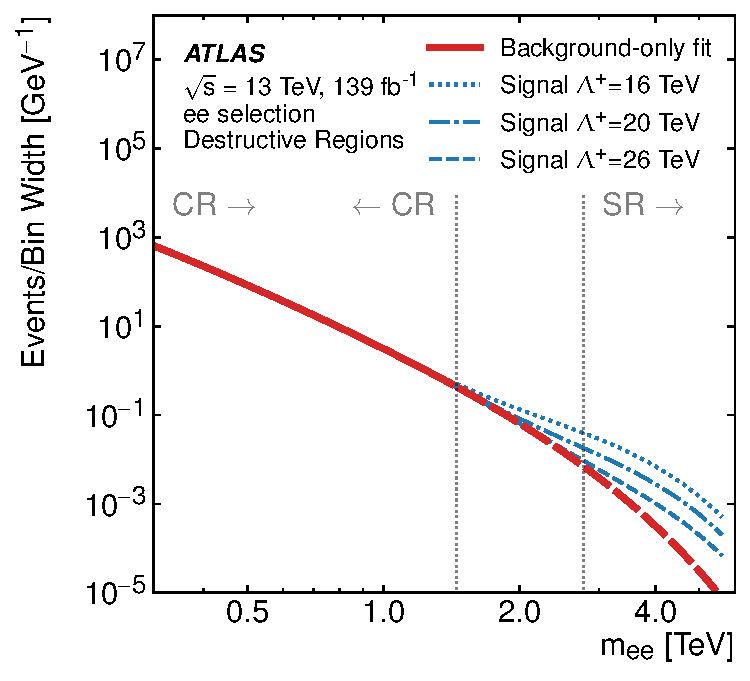
\includegraphics[width=0.45\textwidth]{figures/ci/sigRatio/figaux_01b.pdf}}} \\
\subfloat[][]{{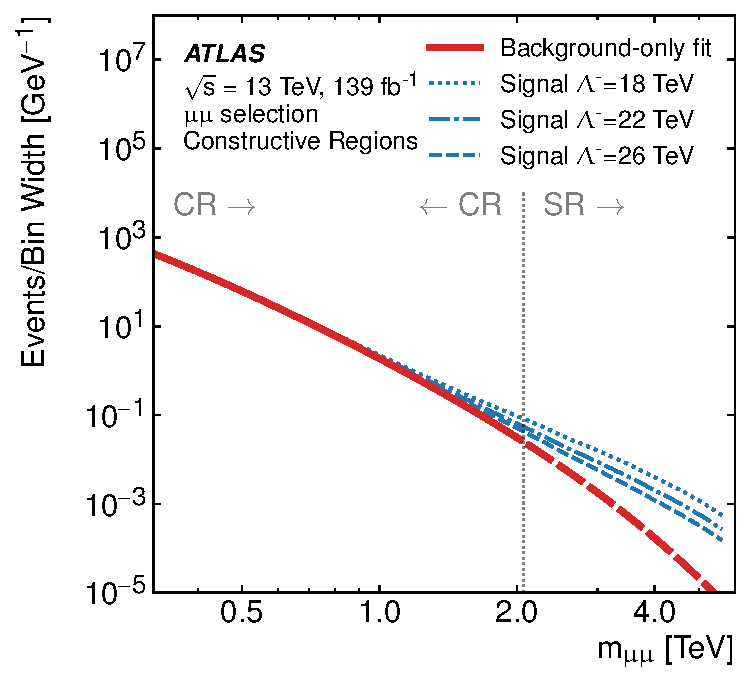
\includegraphics[width=0.45\textwidth]{figures/ci/sigRatio/figaux_02a.pdf}}}
\subfloat[][]{{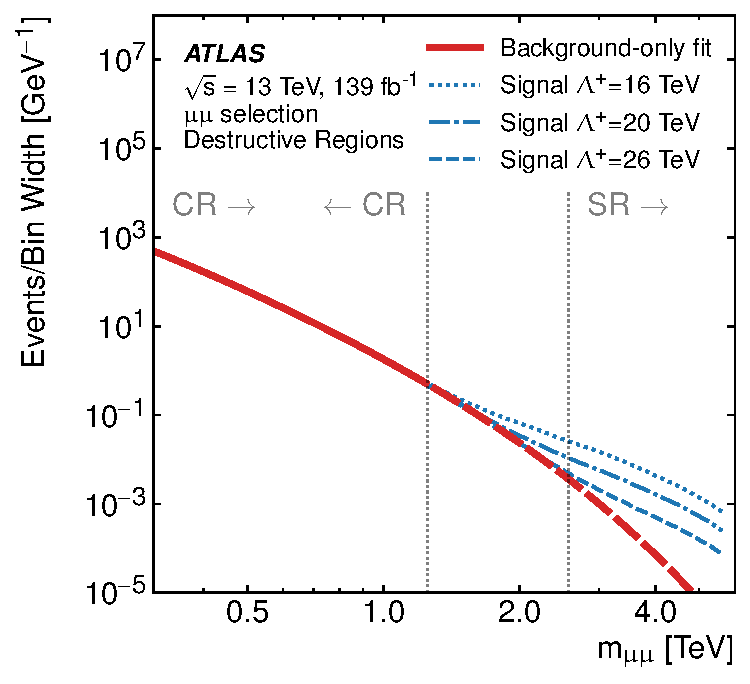
\includegraphics[width=0.45\textwidth]{figures/ci/sigRatio/figaux_02b.pdf}}}
\caption{Signal and background only shapes for the \ee channel (top) and \mm channel (bottom). Constructive signal shapes are shown on the left, and destructive signal shapes are shown on the right. The background shape is derived from a fit of the background model's functional form to the data in the control region. The signal shapes are signal shapes described in the text, added to the background model fit to data.}
\label{fig:ciSignalShape}
\end{center}
\end{figure}
\clearpage
}

% Morphing
The CI signal samples are generated in discrete steps, but it is useful to have a continuous signal description for arbitrary \lam.
Several RooFit classes were developed to interpolate between the generated CI samples smoothly.
\begin{itemize}
    \item A PDF class handles the shape, depending on \lam. This takes a number of input histograms. It interpolates between the histograms' bins to the nearest \mll and between the closest histograms to a particular \lam.
    \item A normalization class handles the normalization of the signal shape, depending on \lam.
\end{itemize}
The advantage of this implementation is that the signal model is compatible with all the fitting and limit setting operations performed with RooFit.
The \lam parameter can be adjusted by RooFit, resulting in a smoothly changing PDF and normalization.

% Morphing interpolations
The PDF class performs two interpolations.
First, a linear interpolation is made between the histogram bin values.
This is used to prevent RooFit from getting stuck while calculating the integral of the PDF (when RooFit sees a discontinuity, it tends to get stuck looking for a delta function).
The second interpolation is between \lam values for different histograms.
This procedure is called \emph{morphing}.

As opposed to a model with a floating signal strength $\mu$, the utility of this morphed model is clear in these plots.
For constructive cases, the signal shapes are roughly the same for different \lam.
In this case, there is an approximate relationship between $\mu$ and \lam, so a fit using a fixed $\Lambda=20$ TeV where $\mu$ is adjusted could represent, for example, $\Lambda=30$ TeV.
This is not the case for the destructive case, as seen in the figures.
The cross over where the signal contribution becomes negative changes with \lam, while it would not change when scaling a given model by $\mu$.
In fact, there are also subtle differences between the constructive signal shapes.
Using the model in terms of \lam makes the constructive signal model more accurate.

Another motivation for using \lam as the parameter-of-interest (POI) in the S+B model is that this maps more directly onto the physics of the problem.
When searching for a resonance, it is natural that the POI be the signal strength $\mu$.
This is both the parameter dictating the strength of the signal and the  parameter on which limits are set.
Likewise, when searching for a contact interaction, the signal's strength is determined by \lam, and the analysis interest is in setting limits on \lam.
There is no physical motivation for a $\Lambda=20$ TeV model scaled by $\mu>1$ to try to represent $\Lambda=10$ TeV. Instead, the morphed signal model allows limits to be set on \lam directly.

Several examples of the morphed signal model are shown in Figures \ref{fig:ciSigModelTemplateCompConst} and \ref{fig:ciSigModelTemplateCompDest}, for constructive and destructive interference patterns respectively.

\afterpage{
\begin{figure}[htp]
\centering
\vspace{-1.0em}
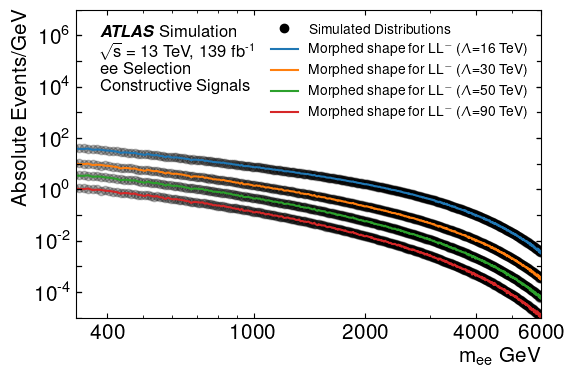
\includegraphics[width=0.45\textwidth]{figures/ci/morphedPdf/sigComp-const-LL-ee.png}
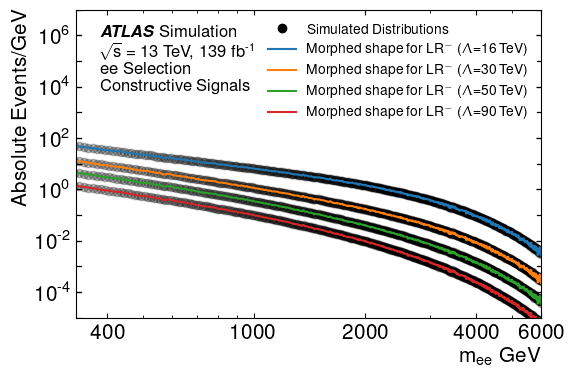
\includegraphics[width=0.45\textwidth]{figures/ci/morphedPdf/sigComp-const-LR-ee.png} \\
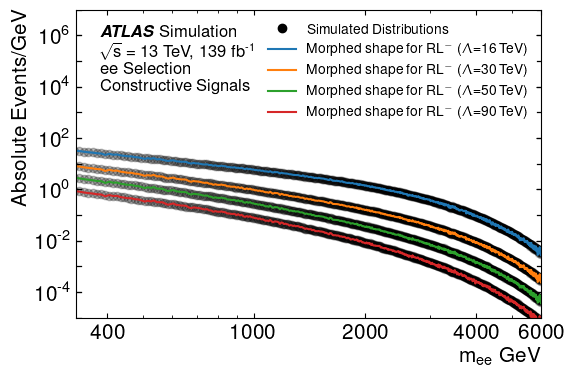
\includegraphics[width=0.45\textwidth]{figures/ci/morphedPdf/sigComp-const-RL-ee.png} 
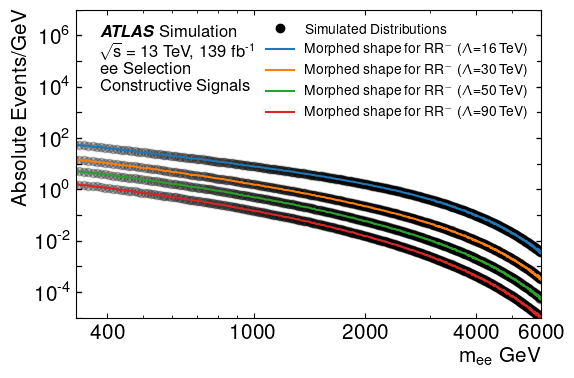
\includegraphics[width=0.45\textwidth]{figures/ci/morphedPdf/sigComp-const-RR-ee.png} \\
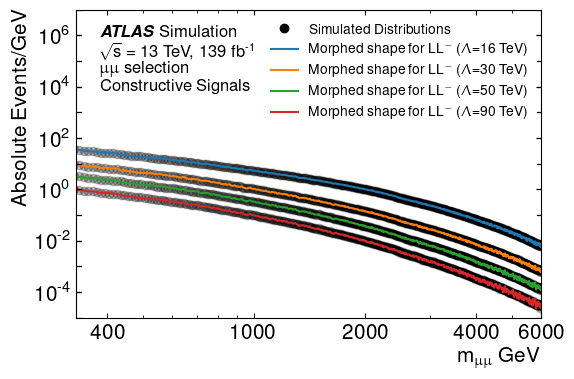
\includegraphics[width=0.45\textwidth]{figures/ci/morphedPdf/sigComp-const-LL-mm.png}
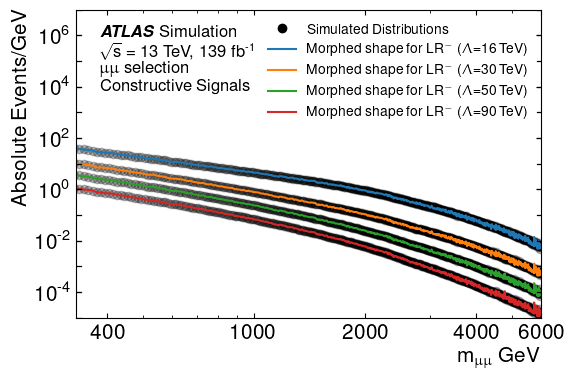
\includegraphics[width=0.45\textwidth]{figures/ci/morphedPdf/sigComp-const-LR-mm.png} \\
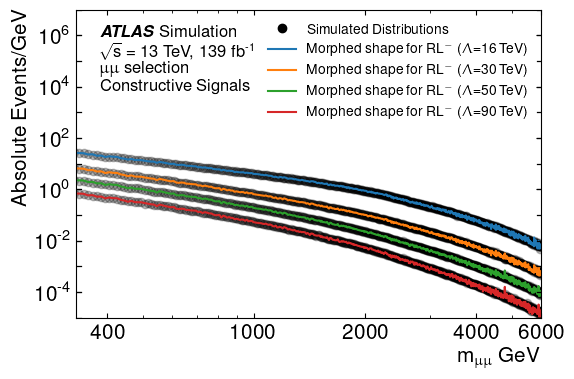
\includegraphics[width=0.45\textwidth]{figures/ci/morphedPdf/sigComp-const-RL-mm.png}
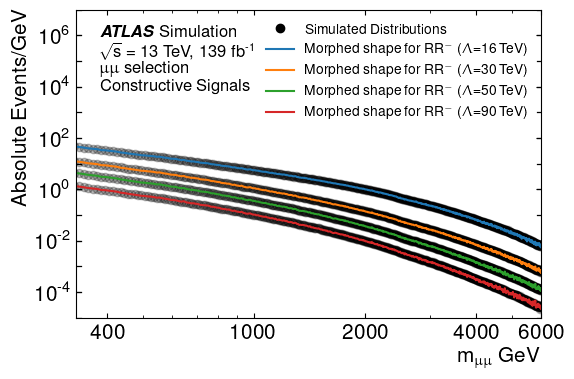
\includegraphics[width=0.45\textwidth]{figures/ci/morphedPdf/sigComp-const-RR-mm.png}
\caption{Comparison between the morphed signal model (colored) and the simulated distributions (black) they are based on.
These are shown for the \ee channel (top) and \mm channel (bottom) constructive interference signals.
}
\label{fig:ciSigModelTemplateCompConst}
\end{figure}
\clearpage
}

\afterpage{
\begin{figure}[htp]
\centering
\vspace{-1.0em}
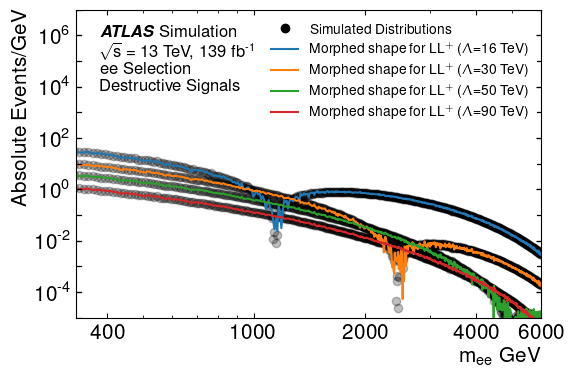
\includegraphics[width=0.45\textwidth]{figures/ci/morphedPdf/sigComp-dest-LL-ee.png}
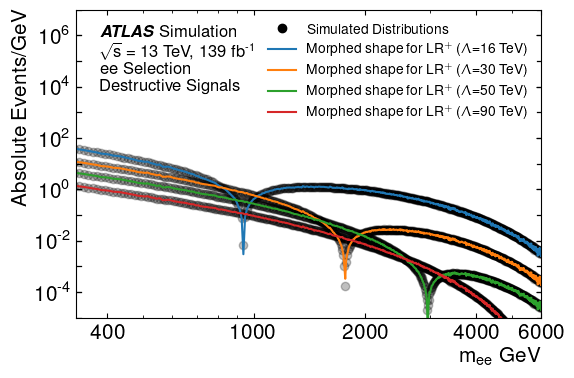
\includegraphics[width=0.45\textwidth]{figures/ci/morphedPdf/sigComp-dest-LR-ee.png} \\
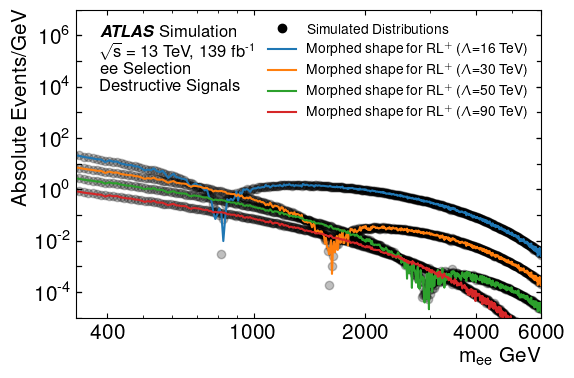
\includegraphics[width=0.45\textwidth]{figures/ci/morphedPdf/sigComp-dest-RL-ee.png} 
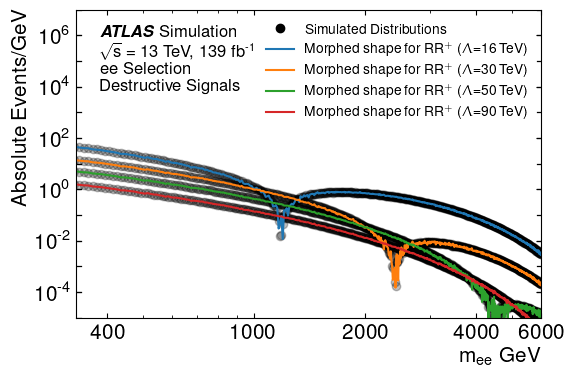
\includegraphics[width=0.45\textwidth]{figures/ci/morphedPdf/sigComp-dest-RR-ee.png} \\
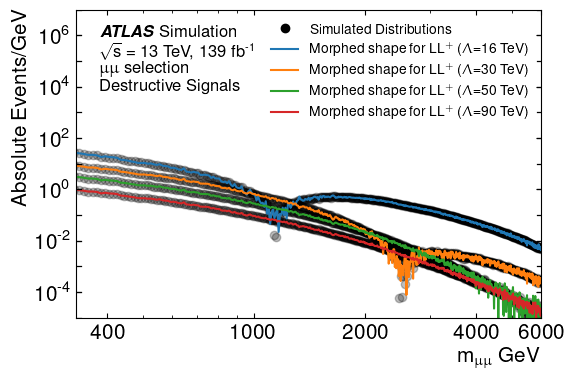
\includegraphics[width=0.45\textwidth]{figures/ci/morphedPdf/sigComp-dest-LL-mm.png}
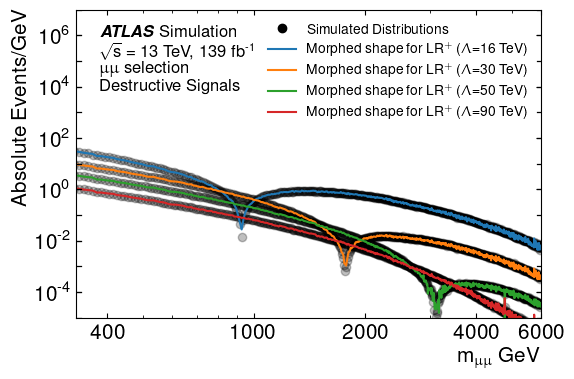
\includegraphics[width=0.45\textwidth]{figures/ci/morphedPdf/sigComp-dest-LR-mm.png} \\
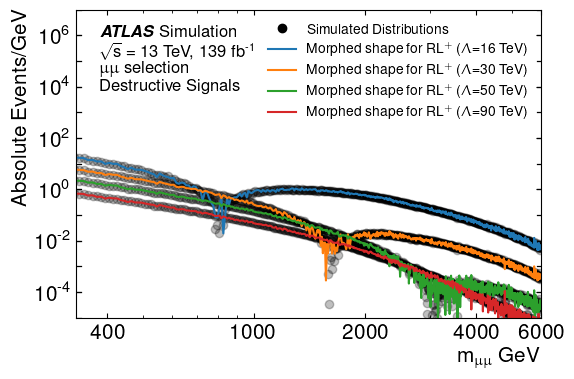
\includegraphics[width=0.45\textwidth]{figures/ci/morphedPdf/sigComp-dest-RL-mm.png}
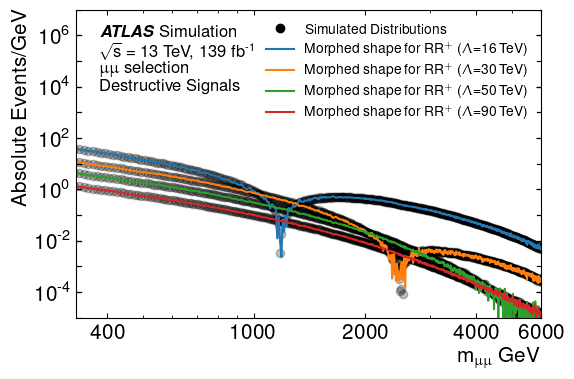
\includegraphics[width=0.45\textwidth]{figures/ci/morphedPdf/sigComp-dest-RR-mm.png}
\caption{Comparison between the morphed signal model (colored) and the simulated distributions (black) they are based on.
These are shown for the \ee channel (top) and \mm channel (bottom) destructive interference signals.
The absolute scale of the vertical axis causes a sharp plotting feature when the interference becomes predominantly destructive.
}
\label{fig:ciSigModelTemplateCompDest}
\end{figure}
\clearpage
}


% S+B model
The full signal shape is used in an extension of the background functions, Equations \ref{eqn:ciBkgEe} and \ref{eqn:ciBkgMm}.
A signal shape, based on the morphed CI signals, is added to the background-only shape, producing an S+B functional form:
\begin{align}
\label{eqn:ciSB}
f_\textrm{s+b}(m_{\ell\ell},\Lambda) = N_\textrm{b}\cdot f_\textrm{b}(m_{\ell\ell}) + N_\textrm{s}(\Lambda)\cdot f_\textrm{s}(m_{\ell\ell},\Lambda),
\end{align}
where $f_\textrm{s}(m_{\ell\ell},\Lambda)$ is the signal probability density function and $N_\textrm{s}(\Lambda)$ is the number of signal events in the CR.
Both $f_\textrm{s}(m_{\ell\ell},\Lambda)$ and $N_\textrm{s}(\Lambda)$ are determined by the morphed CI signals.
The parameter $N_\textrm{b}$ is the number of background events in the CR with the constraint $N_\textrm{b}+N_\textrm{s}(\Lambda)=N_\textrm{CR}$.
The functional form of Equation \ref{eqn:ciSB} is useful because, even in when a large signal is present in the CR, the $N_\textrm{s}(\Lambda)\cdot f_\textrm{s}(m_{\ell\ell},\Lambda)$ term absorbs it.
This leaves the background component undeflected by the presence of a signal.
This property is validated through signal-injection tests detailed in Appendix \ref{sec:ciLinearity}.
This makes Equation \ref{eqn:ciSB} a useful tool to constrain the degree to which the background-only functions (\ref{eqn:ciBkgEe} and \ref{eqn:ciBkgMm}) have been deflected by the presence of a signal in the CR.
This will be further discussed, along with other systematic uncertainties, in Section \ref{sec:ciSyst}.

% The real signal: integral in the SR's
The signal model described up until this point is the differential signal shape in the invariant-mass distribution.
However, the analysis of signal regions considers only the number of events in the region as a function of \lam.
Figure \ref{fig:ciNSigInSr} shows the number of events in each signal region, predicted by various interference and chirality models.
Of particular interest, the RR and LL models predict more events than the LR and RL models in the constructive case.
This pattern is reversed for constructive models.
This is due to the projection of the two chirality operators (Equation \ref{eqn:chiralOps}) hidden in the left and right-handed fermion fields of the Lagrangian (Equation \ref{eqn:ciLagrangian}).
The pattern of varying multiplicity seen in Figure \ref{fig:ciNSigInSr} will later manifest itself in the strength of limits on various CI models.

\afterpage{
\begin{figure}[htp]
\centering
\subfloat[][]{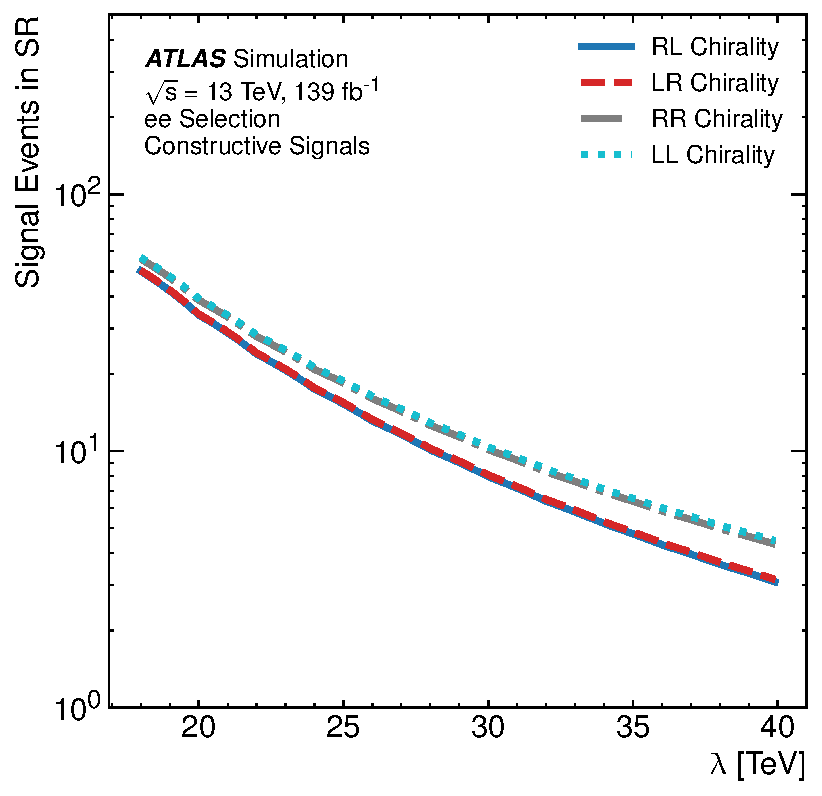
\includegraphics[width=0.449\textwidth]{figures/ci/signalInSr/nSigFunc-ee-const.pdf}}
\subfloat[][]{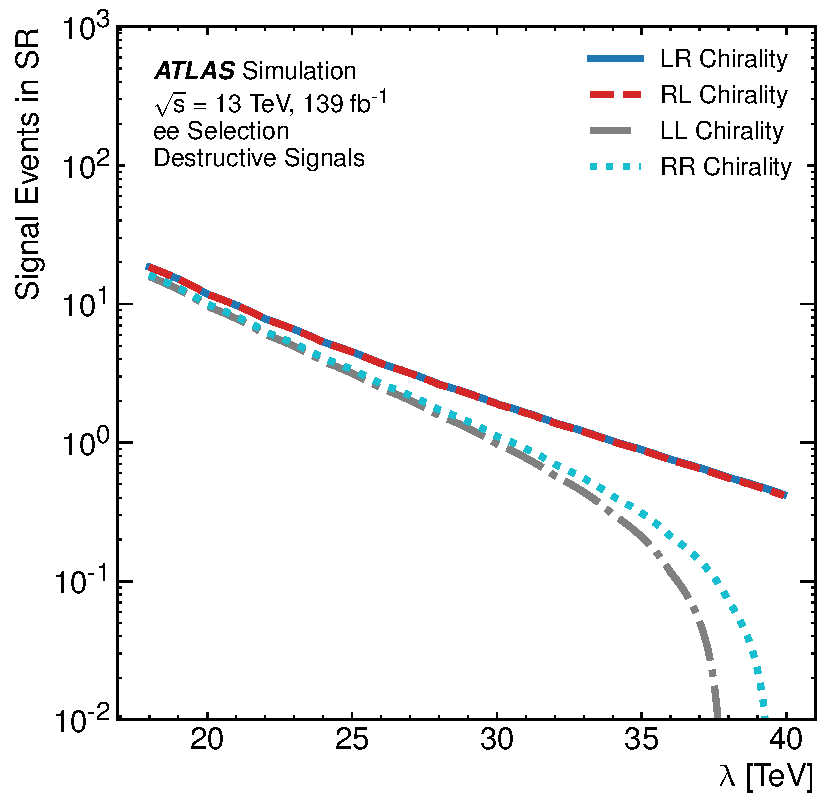
\includegraphics[width=0.449\textwidth]{figures/ci/signalInSr/nSigFunc-ee-dest.pdf}} \\
\subfloat[][]{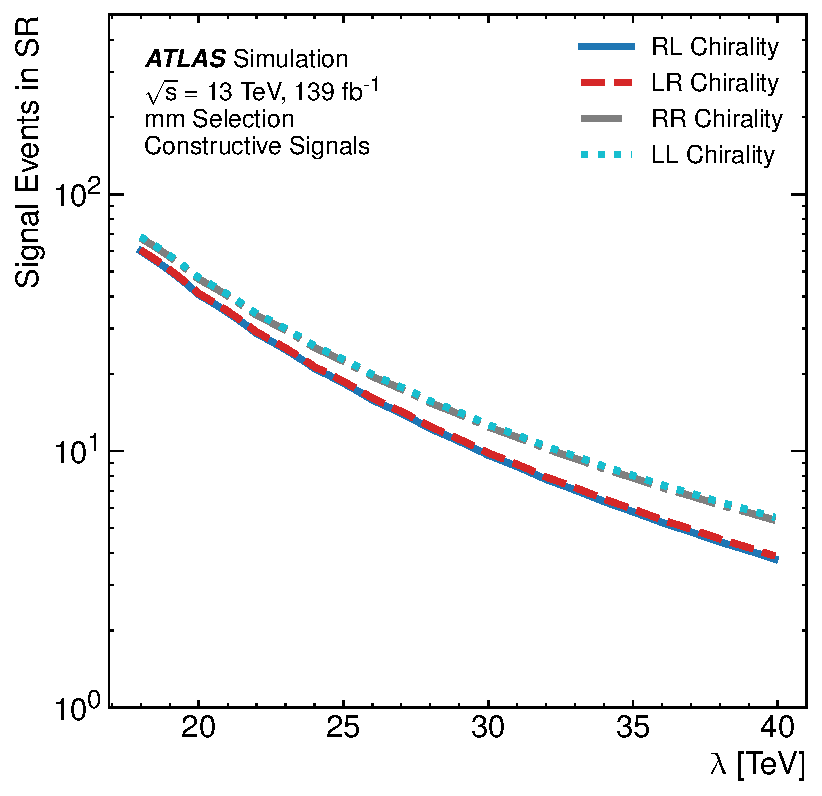
\includegraphics[width=0.449\textwidth]{figures/ci/signalInSr/nSigFunc-mm-const.pdf}}
\subfloat[][]{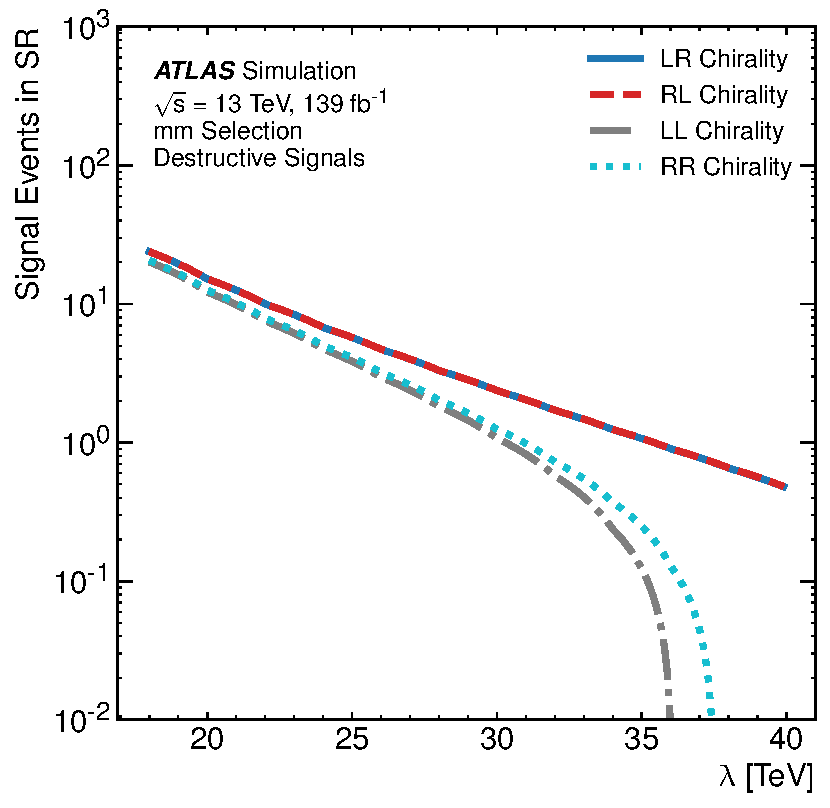
\includegraphics[width=0.449\textwidth]{figures/ci/signalInSr/nSigFunc-mm-dest.pdf}}
\caption{The number of signal events using the morphed model of signal events in each of the four SR's used in the analysis: $ee$-const, $ee$-dest, $\mu\mu$-const, $\mu\mu$-dest in a, b, c, d respectively. Each plot shows the number of signal events as a function of $\Lambda$ for the four chiralities.}
\label{fig:ciNSigInSr}
\end{figure}
\clearpage
}

\afterpage{
\begin{figure}[tb]
\begin{center}
\subfloat[][]{{\includegraphics[width=0.45\textwidth]{figures/ci/sigRatio/figaux_04a.pdf}}}
\subfloat[][]{{\includegraphics[width=0.45\textwidth]{figures/ci/sigRatio/figaux_04b.pdf}}} \\
\subfloat[][]{{\includegraphics[width=0.45\textwidth]{figures/ci/sigRatio/figaux_04c.pdf}}}
\subfloat[][]{{\includegraphics[width=0.45\textwidth]{figures/ci/sigRatio/figaux_04d.pdf}}}
\caption{Signal templates for the CI LL model with constructive (left) and destructive (right) interference for the  dielectron channel is presented for 4 \lam values. The reweighted templates are produced from the same DY sample, therefore the same statistical fluctuations of the underlying DY show up in the plots for each \lam. Also, while the ratio tends to blow up at high mass, this is due to the small number of events in the denominator (DY). In the destructive case, the $\Lambda=30$ TeV signal is still primarily destructive at 2 TeV, but it also has a constructive component at $\approx2.5$ TeV.}
\label{fig:ciSignalRatiosToNominal}
\end{center}
\end{figure}
\clearpage
}

\section{Uncertainties}\label{sec:ciSyst}

For each hypothesis test performed in this analysis, the null hypothesis is termed ``background-only,'' and the alternative hypothesis is termed ``signal+background''.
Both of these hypotheses predict an event yield in a signal region.
The background-only hypothesis is derived from the background model described in Section \ref{sec:ciSig}.
The uncertainties corresponding to its prediction are the uncertainties on the background model and are described in Section \ref{sec:ciSystBkg}.
Alternatively, the signal+background hypothesis also predicts a contribution to the event yield from a signal process.
The uncertainties corresponding to its prediction come both from the background model and the signal process; these are described in Sections \ref{sec:ciSystBkg} and \ref{sec:ciSystSig} respectively.
The groundwork for these uncertainties is described first in Section \ref{sec:ciSystVars}.

\subsection{Simulated Background Variations}\label{sec:ciSystVars}

A number of experimental and theoretical variations on the background shape are used in constructing the uncertainties on the background model and the signal processes.
The variations considered are due to theoretical and experimental uncertainties in the simulated background, as well as those due to the uncertainties in the backgrounds from multi-jet and $W$+jets processes.
The largest source of uncertainty in the simulated background is theoretical, and it is particularly large at the high end of the dilepton mass spectrum.
The second largest source of uncertainty in the simulated background is experimental and is mostly due to high-$p_\text{T}$ muon identification in the dimuon channel.
The third largest source is the uncertainty in the multi-jet and $W$+jets background components and is estimated from the data.
Together, these uncertainties are referred to as \emph{systematic variations} and are used to study the signal and background uncertainties.

\subsubsection{Theoretical Simulated Systematics}\label{sec:ciThySyst}


The following variations are considered for the theoretical uncertainties for the DY component only: the eigenvector variations of the nominal PDF set, variations of PDF scales, the strong coupling ($\alpha_{\textrm S}(M_Z)$), electroweak corrections, photon-induced corrections \cite{Martin:2005pi}, as well as the effect of choosing different PDF sets.
For all PDF variations, the modified DY component is used along with the other nominal background components.
These theoretical uncertainties are the same for both dilepton channels at generator level, but they result in different uncertainties at reconstruction level due to the different resolutions of the dielectron and dimuon channels.
% Further details of this procedure can be found in Ref.~\cite{EXOT-2016-05}.
The size of these uncertainties in the total simulated background is $\leq 19\%$ ($\leq 15\%$) below 4000~GeV for the dielectron (dimuon) channel.

\begin{figure}[htp]
\centering
\subfloat[][]{{\includegraphics[width=0.45\textwidth]{figures/ci/bkgVarRatios/pdfComp-ee.pdf}}}
\subfloat[][]{{\includegraphics[width=0.45\textwidth]{figures/ci/bkgVarRatios/pdfComp-mm.pdf}}}
\caption{Illustration of theory variation shapes, shown as a ratio to the nominal MC, for $ee$ channel (a) and $\mu\mu$ channel (b). Two things are clear from these plots: the impact of the uncertainty in the PDF on $m_{ll}$, and that the impact grows with mass.}
\label{fig:ciThyVar}
\end{figure}

The theoretical systematic uncertainties are used to produce variations on the invariant-mass spectra.
These are illustrated in Figure \ref{fig:ciThyVar}.


% \begin{table}[htp]
%     \centering
%     \begin{tabular}{c}
%     \toprule
%     PDF Variations \\
%     \midrule
%     ALPHAS \\
%     PDF EW \\
%     PI \\
%     PDF Eigenvector Variation 1 \\
%     PDF Eigenvector Variation 2 \\
%     PDF Eigenvector Variation 3 \\
%     PDF Eigenvector Variation 4 \\
%     PDF Eigenvector Variation 5 \\
%     PDF Eigenvector Variation 6 \\
%     PDF Eigenvector Variation 7 \\
%     SCALE Z \\
%     REDCHOICE NNPDF30 \\
%     CHOICE HERAPDF20  \\
%     CHOICE NNPDF30 \\
%     SCALE Z 1up \\
%     Without Run2 FakesTemplate \\
%     Run2 FakesTemplate x3 \\
%     Run2 FakesTemplate x2 \\
%     \bottomrule
%     \end{tabular}
%     \caption{Breakdown of variations of the nominal background included in the calculation of the ISS. These include the fake template variations, PDF choice, eigenvector and scale variations.}
%     \label{tab:ISSBreakdown}
% \end{table}

\subsubsection{Experimental Uncertainty}\label{sec:ciExpSyst}

Uncertainty about the response and performance of the detector leads to systematic experimental uncertainties.
Among the experimental uncertainty sources in the dielectron channel, the dominant ones are the electron identification at low dielectron masses ($\leq 5\%$, below $\sim2000$~GeV) and the uncertainty in the electromagnetic energy scale at higher dielectron masses ($\leq 15\%$).
In the muon channel, the dominant experimental uncertainties arise from the muon reconstruction efficiency at low dimuon masses ($\leq 20\%$, below $\sim4000$~GeV) and from the identification of high-\pt muons at higher dimuon masses ($\leq 50\%$).
The full set of experimental uncertainties are illustrated for the each channel in Figure \ref{fig:ciExpVar}.

\afterpage{
\begin{figure}[h!]
\captionsetup[subfigure]{position=b}
\centering
\includegraphics[width=0.95\textwidth]{figures/ci/bkgVarRatios/pdfComp-ee-det.pdf}\\
\includegraphics[width=0.95\textwidth]{figures/ci/bkgVarRatios/pdfComp-mm-det.pdf}
\caption{Ratio of the background variations to the nominal background estimate for the detector systematic variations in the (top) \ee and (bottom) \mm channels. The prominent variations are numbered.}
\label{fig:ciExpVar}
\end{figure}
\clearpage
}

% \begin{figure}[htp]
% \centering
% \begin{overpic}[width=1\textwidth]{figures/ci/bkgVarRatios/pdfComp-ee-det.pdf}\put(85,0){}\end{overpic}
% \caption{Ratio of the background variations to the nominal background estimate for the detector systematic variations in the electron channel. The prominent variations are numbered.}
% \label{fig:ciExpVarEe}
% \end{figure}

% \begin{figure}[htp]
% \centering
% \begin{overpic}[width=1\textwidth]{figures/ci/bkgVarRatios/pdfComp-mm-det.pdf}\put(85,0){}\end{overpic}
% \caption{Ratio of the background variations to the nominal background estimate for the detector systematic variations in the muon channel. The prominent variations are numbered.}
% \label{fig:ciExpVarMm}
% \end{figure}

\subsubsection{Multijet Electron Background}

The relative uncertainty of the simulated background due to the multi-jet and $W$+jets component rises from $\sim1\%$ at 1~TeV to $\sim10\%$ at 4~TeV.
For the multi-jet and $W$+jets component variations, the modified shape is used each time along with the other nominal background components from the simulation.
This contribution is the smallest amongst all other variations in the CR.

\subsection{Background Estimate}\label{sec:ciSystBkg}
The background estimate described in Section \ref{sec:ciBkg} predicts an event yield in the signal region, based on a functional form fit to the events observed in a control region.
Several assumptions are made in order to interpret this estimate as the prediction of the background hypothesis.
Each assumption is made with a degree of uncertainty.
This is quantified by the three systematic uncertainties described here: the extrapolation uncertainty, the induced spurious-signal (ISS) uncertainty, and the function bias (FB) uncertainty.

The extrapolation and ISS uncertainties are the dominant uncertainties on the background estimate.
These are both measured using statistical ensembles.

\subsubsection{Extrapolation Uncertainty}
\begin{figure}[h!]
\captionsetup[subfigure]{position=b}
\centering
\subfloat[][]{{\includegraphics[width=0.25\textwidth]{figures/ci/iss/fitSs-ee-const.pdf}}} 
\subfloat[][]{{\includegraphics[width=0.25\textwidth]{figures/ci/iss/fitSs-ee-const.pdf}}} 
\subfloat[][]{{\includegraphics[width=0.25\textwidth]{figures/ci/iss/fitSs-ee-const.pdf}}} 
\subfloat[][]{{\includegraphics[width=0.25\textwidth]{figures/ci/iss/fitSs-ee-const.pdf}}} 
\caption{Distributions of the differences between fits to the nominal dataset, and the toy datasets, for each SR.}
\label{fig:ciBkgEuSyst}
\end{figure}

The leading uncertainty on the estimated background is named the extrapolation uncertainty.
The functional form is fit in the CR to data collected in that region.
Since many events occupy each CR ($\approx$72k muons and $\approx$54k electrons), the shape of the \mll data distribution approximates the shape of the underlying truth-PDF that generated it.
However, this approximation is not perfect due to statistical fluctuations in the CR.
The extrapolation uncertainty quantifies the degree to which statistical fluctuations in the CR may lead to varying background estimates in the SR.

This sort of uncertainty is present in other searches and is sometimes called a ``function choice'' uncertainty.
Previously this has been estimated by comparing the result of choosing different functional forms to fit to the data \cite{wprime}.
It is also possible to estimate this impact by looking at the constraints on and covariance of individual parameters of the functional form.
The procedure detailed here forgoes these estimates for a more direct measurement of the impact of statistical fluctuations on the estimated background.

To measure this impact, the background functional form is fit to the data in each CR.
This produces a smooth, \emph{nominal-PDF} that is the best available estimate of truth-PDF.
The background estimate from this fit in the SR defines $N_\text{bkg}^\text{Fit Nominal}$.
The nominal-PDF is used to generate an ensemble of \emph{pseudo-experiments}: toy datasets in the CR invariant-mass region with a multiplicity matching the dataset.
\footnote{There is no uncertainty as to the multiplicity of the actual dataset, and so this exactly determines the toy dataset multiplicity. An alternative option would be to allow $\sqrt{N}$ fluctuation of the multiplicity of each toy. In this case, the toy datasets correspond to the thought experiment: ``if Run 2 had been repeated, lasting for the same duration, what dataset may have been collected?'' This is not the precise thought experiment of interest. Instead, because a fixed number of events have already been sampled from the truth-PDF, it is asked: ``if an alternative sampling of the truth-PDF had taken place, what dataset may have been collected?''}
Each toy dataset is then fit using the background functional form and the resulting function is extrapolated to the SR to provide a toy background estimate $N_{\text{bkg},i}^\text{Fit Toy}$.
A comparison is made between the background estimate from the fit to the toy dataset and the nominal fit for each toy $i$:
\begin{equation*}
    \Delta_i^\text{stat}=N_{\text{bkg},i}^\text{Fit Toy}-N_\text{bkg}^\text{Fit Nominal}.
\end{equation*}
This defines the degree, $\Delta_i^\text{stat}$, to which statistical effects in the CR have altered the background estimate.


This procedure is repeated with an ensemble of 2,000 toy datasets.
The distribution of $\Delta_i^\text{stat}$ values is built from each fit. These are shown in Figure \ref{fig:ciBkgEuSyst} for each SR.
The standard deviation of these distributions is taken to define the systematic error on the background expectation due to the extrapolation uncertainty.

\subsubsection{Induced Spurious-Signal}



% What needs to be measured
The sub-leading uncertainty on the background estimate is called the induced spurious-signal (ISS) uncertainty.
This quantifies the systematic difference between the background model and the true underlying background-only distribution in the SR.
The ISS how well the background model can be expected to model the underlying physical distribution from which the data has been sampled.
If the background functional form were to fit the true background-PDF, then the difference between the fitted function and normalized PDF in the CR is the ISS.
Since any mis-modeling of the background, on average, leads to the identification of a signal even in the background-only scenario, this mis-modeling is called a \emph{spurious-signal}.

% Challenge with measuring it
The ISS can not be measured directly, since the background-PDF is unknown.
Furthermore, it is inaccurate to use the simulated background-only dataset to measure the ISS because this makes the improper assumption that the nominal simulation matches the shape of the true background-PDF.
Instead, a new methodology called the \emph{statistical background ensemble} was developed to measure the ISS.
The general theoretical motivation for the methodology is described in Appendix \ref{sec:backgroundEnsamble}.
The method seeks to measure the ISS from an ensemble of possible background shapes, each weighted by a prior likelihood.
The prior likelihoods are derived from the systematic variations discussed in Section \ref{sec:ciSystVars}.

The space of all plausible background shapes is described by linear combinations of the $n$ systematic variations.
Each of these is identified by a corresponding $n$-vector $\vec{\theta}$.
Each choice of $\vec{\theta}$ corresponds to a background shape $B'$:
\begin{equation}\begin{split}
    B'(\mll,\vec{\theta}) = B_\text{Nominal}(\mll) + \sum_{i=1}^n \omega_i(\mll)*\theta_i,
\end{split}\end{equation} 
where $\omega_i$ correspond to the shapes of the systematic variations.
The $\omega_i$ shapes can be normalized to correspond to $1\sigma$ deviations from the nominal shape.
In this case, $\theta_i=1$ corresponds to a $+1\sigma$ deviation, while $\theta_i=-1$ corresponds to a $-1\sigma$ deviation.
Several toy background shapes are illustrated in Figure \ref{fig:bkgToyEnsamble}.


If the systematic variations are taken to define prior probabilities for nuisance parameters $\theta_i$, then the prior probability of $\vec{\theta}$ corresponding to the true background shape is:
\begin{equation}\begin{split}
    P(\vec{\theta})=\prod_{i=1}^n \text{G}(\theta_i),
\end{split}\end{equation} 
where $\text{G}(\theta_i)$ are standard normal functions.

In many cases, the systematic uncertainty shape is measured separately for upward and downward fluctuations.
For these systematics, the two shapes $\omega^+_i$ and $\omega^-_i$ are used as appropriate depending on whether $\theta_i$ is positive or negative.

\begin{figure}[h!]
\captionsetup[subfigure]{position=b}
\centering
\subfloat[][]{{\includegraphics[width=0.5\textwidth]{figures/ci/systToys/toy-ee-0-0.pdf}}}
\subfloat[][]{{\includegraphics[width=0.5\textwidth]{figures/ci/systToys/toy-mm-6-6.pdf}}}
\caption{Illustration of four toy backgrounds, $B'$, for the \ee (a) and \mm (b) channel systematics. The nominal background is shown in black, while two toys corresponding to $\vec{\theta}$ and $-\vec{\theta}$ are shown in red and blue. In the upper frames, these are offset by a shift to distinguish the lines.}
\label{fig:bkgToyEnsamble}
\end{figure}

Ideally, the ISS could be measured across the full space of $\vec{\theta}$.
This can be approximated numerically using an ensemble of backgrounds drawn from space of $\vec{\theta}$ randomly weighted by their prior likelihood.
For each of the $n$ systematic variations, a standard Gaussian PDF is sampled to determine the corresponding element of $\vec{\theta}$. \footnote{At the request of the ATLAS Publications Committee, the Gaussians are restricted to $[-1,1]$. This restriction is not impactful.}
The result is that each $\vec{\theta}$ of the ensemble is drawn with a probability proportional to the prior probability of the corresponding background shape.
Then, the background shapes $B'(\mll,\vec{\theta})$ and $B'(\mll,-\vec{\theta})$ are constructed.
The use of both $\vec{\theta}$ and $-\vec{\theta}$ forces a symmetric sampling of the space of $\vec{\theta}$. 
This reduces the size of the ensemble required to sample the vector space.

\begin{figure}[h!]
\captionsetup[subfigure]{position=b}
\centering
\subfloat[][]{{\includegraphics[width=0.25\textwidth]{figures/ci/toyUncert/toyNSSDist-ee-const-all-noGaus.pdf}}}
\subfloat[][]{{\includegraphics[width=0.25\textwidth]{figures/ci/toyUncert/toyNSSDist-ee-dest-all-noGaus.pdf}}} 
\subfloat[][]{{\includegraphics[width=0.25\textwidth]{figures/ci/toyUncert/toyNSSDist-mm-const-all-noGaus.pdf}}}
\subfloat[][]{{\includegraphics[width=0.25\textwidth]{figures/ci/toyUncert/toyNSSDist-mm-dest-all-noGaus.pdf}}}
\caption{Distributions of the Induced Spurious-Signal measured by enables of 2,000 pseudo-experiments. The grey lines show the envelope that contains all spurious-signals measured on individual systematic variations.}
\label{fig:ciBkgIssSyst}
\end{figure}

This process is repeated to build an ensemble of background shapes used to create 2,000 Asimov toy datasets.
Each toy dataset is fit with the nominal background functional form.
A comparison is made between SR yields of the fitted function and the Asimov dataset for each toy $i$:
\begin{equation*}
    \Delta_i^\text{ISS}=N_{\text{bkg},i}^\text{Fit}-N_\text{bkg}^\text{Asimov}.
\end{equation*}
The distribution of $\Delta_i^\text{ISS}$ is built up through 2,000 background shape toys for each SR, as shown in Figure \ref{fig:ciBkgIssSyst}.
The mean of these distributions defines the measurement of the ISS of the background model in each SR.
The width of these distributions is the uncertainty corresponding to that measurement.
The mean and standard deviation of the distribution are added in quadrature as the estimate of the ISS for the underlying background-PDF.

\subsubsection{Function Bias Uncertainty}

The remaining uncertainty on the background estimate is the function bias (FB) uncertainty.
This uncertainty describes the degree to which a signal, if present in the CR, may potentially bias the background expectation in the SR.
The function bias uncertainty is measured using the background expectations derived from the S+B functional form Equation \ref{eqn:ciSB}.
This is compared to the analogous background expectation from the B-only functional form from Equations \ref{eqn:ciBkgEe} and \ref{eqn:ciBkgMm}.
Each functional forms is fit to the observed data in each control region.
The difference between the background estimates from the S+B and B-only fits defines the function bias uncertainty.
For each lepton flavor channel and CI interference combination there are four S+B functional forms corresponding to the LL, LR, RL, and RR chiralities.
Since the FB uncertainties measured for each chirality are observed to have similar magnitudes, the largest FB is used for each lepton channel and interference combination.

The motivation for the FB uncertainty is based on the flexibility of the S+B model to adapt to cases where a signal is present in the CR.
This property is illustrated in Appendix \ref{sec:ciLinearity}.
As a result, the FB uncertainty is taken to constrain the degree to which, if present in the CR, a signal shape may distort the background expectation from the B-only functional form.

The FB uncertainty is small by construction.
If, when measured on data for a given control region, the value had been significant compared to extrapolation and ISS uncertainties, then this would have invalidated the choice of CR by indicating the presence of a signal-like feature.
A procedure was defined before any observation of data to handle this eventuality.
The high-mass limit of the CR would be lowered until the bias vanished, with no adjustment to the SR. 
Because the non-resonant signals of interest vanish towards low-mass, reducing the upper limit of the CR would eventually remove the contribution from such a signal.

In the observed data, none of the function bias measurements are significant compared to the dominant uncertainties on the background model.
Indeed, the impact on the expected sensitivity is under 2\%.
This uncertainty is only considered for the limits on the contact interaction energy scale \lam since it depends on the shape of those signals.

% The results of the function bias measurement are shown in Figure \ref{fig:ciFuncBias}.
% This measurement is repeated for each SR and each chirality model.
% A conservative choice of the largest bias for any given chirality is selected.

% \afterpage{
% \begin{figure}[!htb]
% \begin{center}
% \subfloat[][]{{\includegraphics[width=0.24\textwidth]{figures/ci/bkgCompat-final/nbkg-LL-const-ee.png}}}
% \subfloat[][]{{\includegraphics[width=0.24\textwidth]{figures/ci/bkgCompat-final/nbkg-LR-const-ee.png}}}
% \subfloat[][]{{\includegraphics[width=0.24\textwidth]{figures/ci/bkgCompat-final/nbkg-RL-const-ee.png}}}
% \subfloat[][]{{\includegraphics[width=0.24\textwidth]{figures/ci/bkgCompat-final/nbkg-RR-const-ee.png}}} \\
% \subfloat[][]{{\includegraphics[width=0.24\textwidth]{figures/ci/bkgCompat-final/nbkg-LL-dest-ee.png}}}
% \subfloat[][]{{\includegraphics[width=0.24\textwidth]{figures/ci/bkgCompat-final/nbkg-LR-dest-ee.png}}}
% \subfloat[][]{{\includegraphics[width=0.24\textwidth]{figures/ci/bkgCompat-final/nbkg-RL-dest-ee.png}}}
% \subfloat[][]{{\includegraphics[width=0.24\textwidth]{figures/ci/bkgCompat-final/nbkg-RR-dest-ee.png}}} \\
% \subfloat[][]{{\includegraphics[width=0.24\textwidth]{figures/ci/bkgCompat-final/nbkg-LL-const-mm.png}}}
% \subfloat[][]{{\includegraphics[width=0.24\textwidth]{figures/ci/bkgCompat-final/nbkg-LR-const-mm.png}}}
% \subfloat[][]{{\includegraphics[width=0.24\textwidth]{figures/ci/bkgCompat-final/nbkg-RL-const-mm.png}}}
% \subfloat[][]{{\includegraphics[width=0.24\textwidth]{figures/ci/bkgCompat-final/nbkg-RR-const-mm.png}}} \\
% \subfloat[][]{{\includegraphics[width=0.24\textwidth]{figures/ci/bkgCompat-final/nbkg-LL-dest-mm.png}}}
% \subfloat[][]{{\includegraphics[width=0.24\textwidth]{figures/ci/bkgCompat-final/nbkg-LR-dest-mm.png}}}
% \subfloat[][]{{\includegraphics[width=0.24\textwidth]{figures/ci/bkgCompat-final/nbkg-RL-dest-mm.png}}}
% \subfloat[][]{{\includegraphics[width=0.24\textwidth]{figures/ci/bkgCompat-final/nbkg-RR-dest-mm.png}}}
% \caption{Background estimate compared in the SR, for B-only and S+B fits to data in each channel. (a-d) show constructive \ee fits for LL, LR, RL, and RR chiralities. (d-h) show the same for destructive \ee. (i-l) show the same for constructive \mm, and (m-p) show the same for destructive \mm.}
% \label{fig:ciFuncBias}
% \end{center}
% \end{figure}
% \clearpage
% }


\subsection{Signal Model}\label{sec:ciSystSig}
The signal models used in this analysis are more traditional than the background model, and therefore the corresponding systematic uncertainties are fairly standard.
There are both experimental and theoretical uncertainties to consider.
The experimental uncertainties, described in Section \ref{sec:ciSigExpSyst}, are applied similarly to the CI signal model and the model-independent signal production.
The theoretical uncertainties, described in Section \ref{sec:ciSigThySyst}, must be considered differently.
The hypothesis test performed by this analysis compares the background hypothesis to the signal+background hypothesis.
The choice of the signal model unambiguous: there is no uncertainty in which signal model is being tested.
Theoretical variations, like the PDF choice and $\alpha_s$ scale, are part of this signal model choice.
Different theoretical choices describe different signal models.
Therefore, these different signal models are tested for in separate hypothesis tests.

\subsubsection{Experimental}\label{sec:ciSigExpSyst}

The experimental uncertainties under consideration are described in Section \ref{sec:ciExpSyst}.
These are produced as functions of invariant-mass \mll.
The impact of each systematic on the CI signal model is the convolution of the CI shape in \mll and the systematic shape in \mll, but this is relatively independent of the signal shape.
For different contact interactions, the impact of experimental systematics generally varies by less than 1\%.
Thus, for simplicity, these are calculated for the LO DY shape in the CR and applied equally for each CI model.
The experimental uncertainties are listed for the \ee channel in Table \ref{tab:ciExpVariationBonanzaEe} and the \mm channel in Table \ref{tab:ciExpVariationBonanzaMm}.
The sum in quadrature of the experimental uncertainties is used to constrain the signal prediction.
The experimental uncertainties of the signal are $\leq 9\%$ for the electron channel and $\leq 22\%$ for the muon channel.


\afterpage{
\begin{table}[]
\begin{center}
\caption{Impact of experimental uncertainties on NLO DY yield in CI signal regions. The total is calculated as the sum in quadrature including contributions from sources of impact $\geq 1\%$.}
\begin{tabular}{c l c c c c}
\toprule
SR &  Source & Uncertainty \\
\midrule
\multirow{9}{*}{\begin{sideways}\ee Destructive\end{sideways}} & EG\_RES & $\sim 0.0\% \ \sim 0.0\%$ \\
& EG\_SCALE & $+ 5.9\% \   -5.8\%$ \\
& EL\_ChargeID & $\sim 0.0\% \ \sim 0.0\%$ \\
& EL\_ID & $+ 5.9\% \   -5.8\%$ \\
& EL\_Iso & $+ 0.8\% \   -0.8\%$ \\
& EL\_Reco & $+ 0.4\% \   -0.4\%$ \\
& EL\_TRIG\_EFF & $\sim 0.0\% \ \sim 0.0\%$ \\
& EL\_TRIG\_TOTAL & $\sim 0.0\% \ \sim 0.0\%$ \\
& PRW & $\sim 0.0\% \   -0.1\%$ \\
 & Total & $+ 8.4\% \   -8.2\%$ \\
\midrule
\multirow{9}{*}{\begin{sideways}\ee Constructive\end{sideways}} & EG\_RES & $\sim 0.0\% \ \sim 0.0\%$ \\
& EG\_SCALE & $+ 5.2\% \   -4.9\%$ \\
& EL\_ChargeID & $\sim 0.0\% \ \sim 0.0\%$ \\
& EL\_ID & $+ 5.9\% \   -5.8\%$ \\
& EL\_Iso & $+ 0.8\% \   -0.8\%$ \\
& EL\_Reco & $+ 0.4\% \   -0.4\%$ \\
& EL\_TRIG\_EFF & $\sim 0.0\% \ \sim 0.0\%$ \\
& EL\_TRIG\_TOTAL & $\sim 0.0\% \ \sim 0.0\%$ \\
& PRW & $\sim 0.0\% \ \sim 0.0\%$ \\
 & Total & $+ 7.9\% \   -7.6\%$ \\
\bottomrule
\end{tabular}
\label{tab:ciExpVariationBonanzaEe}
\end{center}
\end{table}
\clearpage
}

\afterpage{
\begin{table}[]
\begin{center}
\caption{Impact of experimental uncertainties on NLO DY yield in CI signal regions. The total is calculated as the sum in quadrature including contributions from sources of impact $\geq 1\%$.}
\begin{tabular}{c l c c c c}
\toprule
SR &  Source & Uncertainty \\
\midrule
\multirow{16}{*}{\begin{sideways}\mm Destructive\end{sideways}} & MUON\_BADMUON\_STAT & $\sim 0.0\% \ \sim 0.0\%$ \\
& MUON\_BADMUON\_SYS & $+ 7.8\% \   -7.6\%$ \\
& MUON\_ISO\_STAT & $+ 0.3\% \   -0.3\%$ \\
& MUON\_ISO\_SYS & $+ 0.4\% \   -0.4\%$ \\
& MUON\_RECO\_STAT & $+ 0.6\% \   -0.6\%$ \\
& MUON\_RECO\_SYS & $+ 21.7\% \   -19.4\%$ \\
& MUON\_TTVA\_STAT & $\sim 0.0\% \ \sim 0.0\%$ \\
& MUON\_TTVA\_SYS & $\sim 0.0\% \ \sim 0.0\%$ \\
& MUON\_TRIG\_STAT & $\sim 0.0\% \ \sim 0.0\%$ \\
& MUON\_TRIG\_SYS & $+ 0.1\% \   -0.1\%$ \\
& MUON\_ID & $+ 1.0\% \   -1.1\%$ \\
& MUON\_MS & $+ 4.6\% \   -3.7\%$ \\
& MUON\_SAGITTA\_RESBIAS & $+ 12.8\% \ + 5.5\%$ \\
& MUON\_SAGITTA\_RHO & $\sim 0.0\% \ \sim 0.0\%$ \\
& MUON\_SCALE & $  -0.4\% \ + 0.3\%$ \\
& PRW & $\sim 0.0\% \ \sim 0.0\%$ \\
& Total & $+ 26.7\% \   -21.9\%$ \\
\midrule
\multirow{16}{*}{\begin{sideways}\mm Constructive\end{sideways}} & MUON\_BADMUON\_STAT & $\sim 0.0\% \ \sim 0.0\%$ \\
& MUON\_BADMUON\_SYS & $+ 4.0\% \   -3.8\%$ \\
& MUON\_ISO\_STAT & $+ 0.3\% \   -0.2\%$ \\
& MUON\_ISO\_SYS & $+ 0.5\% \   -0.3\%$ \\
& MUON\_RECO\_STAT & $+ 0.6\% \   -0.5\%$ \\
& MUON\_RECO\_SYS & $+ 17.9\% \   -16.1\%$ \\
& MUON\_TTVA\_STAT & $+ 0.1\% \ \sim 0.0\%$ \\
& MUON\_TTVA\_SYS & $\sim 0.0\% \ \sim 0.0\%$ \\
& MUON\_TRIG\_STAT & $+ 0.2\% \ \sim 0.0\%$ \\
& MUON\_TRIG\_SYS & $+ 0.2\% \ \sim 0.0\%$ \\
& MUON\_ID & $+ 0.7\% \   -0.7\%$ \\
& MUON\_MS & $+ 2.7\% \   -2.2\%$ \\
& MUON\_SAGITTA\_RESBIAS & $+ 8.0\% \ + 1.8\%$ \\
& MUON\_SAGITTA\_RHO & $\sim 0.0\% \ \sim 0.0\%$ \\
& MUON\_SCALE & $  -0.4\% \ + 0.4\%$ \\
& PRW & $\sim 0.0\% \ + 0.2\%$ \\
& Total & $+ 20.2\% \   -16.8\%$ \\
\bottomrule
\end{tabular}
\label{tab:ciExpVariationBonanzaMm}
\end{center}
\end{table}
\clearpage
}

\subsubsection{Theoretical Uncertainty}\label{sec:ciSigThySyst}
The theoretical uncertainties under consideration are described in Section \ref{sec:ciThySyst}.
These are useful to provide alternative signal models that correspond to the $1\sigma$ limits on theoretical parameters.
The impact of the theoretical uncertainties on the signal yield is calculated in each SR.
It is equal to the sum in quadrature of the convolution of the theory systematic shapes with the LO DY shape.


\subsection{Summary of Uncertainties}

The numerical values of the uncertainties are given in Table \ref{tab:ciUncerts}.
For all cases, the relative uncertainties in the destructive SRs are larger than those in the constructive SRs.
This is due to both the smaller size of the SR leading to less background and larger relative uncertainty and the smaller size of the CR, leading to a weaker constraint on the background model.
For the background estimates, the leading uncertainty in each SR is the extrapolation uncertainty, followed by the ISS uncertainty.
Many of the experimental and theoretical systematics are measured separately for upward and downward fluctuations.


\begin{table}[!h]
\begin{center}
\caption{Summary of the relative uncertainties in the background estimate and signal in each SR, where EU is the `extrapolation uncertainty', ISS is the `induced spurious-signal uncertainty' and FB is the `function bias uncertainty'. Experimental and theoretical uncertainties are shown as well, with the latter averaged across CI chirality scenarios and quoted for $\Lambda=30$~TeV only.}
\begingroup
\setlength{\tabcolsep}{10pt} % Default value: 6pt
\renewcommand{\arraystretch}{1.5} % Default value: 1
{\small
% \begin{tabular}{l l | r r r | r r r r}
\begin{tabular}{l l | r r r | r@{}l r@{}l}
% \Xhline{2\arrayrulewidth}
\toprule
\multirow{2}{*}{Channel} & \multirow{2}{*}{Interference} & \multicolumn{3}{c|}{Background uncertainties} & \multicolumn{4}{c}{Signal uncertainties}\\
        &              & $\sigma_b^\text{EU}$ & $\sigma_b^\text{ISS}$ & $\sigma_b^\text{FB}$ & \multicolumn{2}{c}{$\sigma_s^\text{Experiment}$} & \multicolumn{2}{c}{$\sigma_s^\text{Theory}$} \\
\midrule
\ee     & Constructive & 14\% & 4\%  & 2\% & 8&\%                               & \makecell[r]{+11 \\ --10}&\makecell[l]{\% \\ \%} \\
\ee     & Destructive  & 34\% & 7\% & 1\%  & 8&\%                               & \makecell[r]{+14 \\ --13}&\makecell[l]{\% \\ \%} \\
$\mm$ & Constructive & 21\% & 6\%  & 2\% & \makecell[r]{+20 \\ --17}&\makecell[l]{\% \\ \%} & \makecell[r]{+10 \\ --9}&\makecell[l]{\% \\ \%} \\
$\mm$ & Destructive  & 58\% & 24\% & 4\% & \makecell[r]{+27 \\ --22}&\makecell[l]{\% \\ \%} & \makecell[r]{+13 \\ --12}&\makecell[l]{\% \\ \%} \\
% \Xhline{2\arrayrulewidth}
\bottomrule
\end{tabular}
}
\endgroup
\label{tab:ciUncerts}
\end{center}
\end{table}

\section{Statistical Analysis}\label{sec:ciStat}

Statistical methods are used to distill two types of information from the collected dataset.
First, to determine the probability that the observed data is incompatible with the background-only (B-only) hypothesis.
Second, to determine the smallest putative signal such that, if extant, would produce a signal+background (S+B) hypothesis that is incompatible with the observed data.
The former is answered by a significance test, described in Section \ref{sec:ciSigTest}, while the latter is answered by setting a limit, described in Section \ref{sec:ciLimitSetting}.

\subsection{Likelihood Ratio and CLs Method}

\begin{figure}[h!]
\captionsetup[subfigure]{position=b}
\centering
\subfloat[][]{\label{fig:ciClsNobs}{\includegraphics[width=0.5\textwidth]{figures/stats/stat-nobs.pdf}}}
\subfloat[][]{\label{fig:ciClsProfileLikelihood}{\includegraphics[width=0.5\textwidth]{figures/stats/stat-likel.pdf}}}
\caption{PDFs predicted by S+B and B-only hypotheses of test statistics (a) \nobs and (b) the likelihood ratio. Note the log scale of (b). In each case, the shaded regions mark the set of test statistic values for which each hypothesis would be more incompatible then with the observed value shown in grey.}
\label{fig:ciCls}
\end{figure}

% \begin{figure}[h!]
% \captionsetup[subfigure]{position=b}
% \centering
% \includegraphics[width=0.5\textwidth]{figures/ci/profileLikelihoodPlots/toys-n29-fc-lambda-ll-const-LL-nToy5000-nSteps50-seed8.png}
% \caption{}
% \label{fig:ciClsProfileLikelihood}
% \end{figure}

% Test statistic: likelihood ratio
The fundamental tool used to compare two hypotheses is the \emph{test statistic}, a quantity calculated from the observed data.
Each hypothesis predicts a probability density function (PDF) that describes the probability to observe values of the test statistic.
The PDF of the B-only hypothesis, $\mathcal{L}(\nobs)$, is a function of the test statistic \nobs.
Composite hypotheses are more useful and are defined by additional parameters, $\theta$, that may be estimated from the observation.
In general, a B-only hypothesis defined by $\theta_0$ predicts a PDF of $\mathcal{L}(\nobs|\theta_0)$, while an S+B hypothesis defined by $\theta_1$ predicts a PDF of $\mathcal{L}(\nobs|\theta_1)$.
For example, a B-only hypothesis may predict a Gaussian PDF with a mean that is smaller than the average predicted by an S+B hypothesis.
An illustration is shown in Figure \ref{fig:ciClsNobs}.
Here, the B-only hypothesis is more compatible with an observation of \nobs=500 than \nobs=1,000, while the converse is true of the S+B hypothesis.
The choice to accept or reject a hypothesis is made by a comparison of their respective PDFs.

While the test statistic may be any quantity calculated from data, an optimal choice for the test statistic may be made to resolve the difference between the two hypotheses.
A common choice is to use the ratio of the S+B and B-only hypotheses to define the \emph{likelihood ratio} in Equation \ref{eqn:ciLikelihoodTestStat}.
\begin{equation}\begin{split}\label{eqn:ciLikelihoodTestStat}
    \Lambda(\nobs)=\frac{\mathcal{L}(\nobs|\theta_1)}{\mathcal{L}(\nobs|\theta_0)},
\end{split}\end{equation} 
The Neyman-Person lemma states that the likelihood ratio test is the most likely to reject the B-only hypothesis, given that the S+B hypothesis is true \cite{eilam}

An example of the PDFs of the likelihood distributions, produced under the assumption of either the S+B or B-only hypotheses, is shown in figure \ref{fig:ciClsProfileLikelihood}.
Measurements of the likelihood ratio test statistic, $\Lambda(\nobs)$, can fall at different points on the horizontal axis.
As in the case of the earlier illustration, the two compatibility of the two hypothesis with the observation may then be assessed.
Data measured at larger values of $\Lambda(\nobs)$ are \emph{less compatible} with the background-only hypothesis.
Likelihood ratios can complicated functions; in practice they usually need be estimated computationally. 

% In practice, the quantity $-\ln{\Lambda(\nobs)}$ is used for computational simplicity.

% \begin{figure}[h!]
% \captionsetup[subfigure]{position=b}
% \centering
% \includegraphics[width=0.5\textwidth]{figures/ci/cls.png}
% \caption{}
% \label{fig:ciClsNobs}
% \end{figure}

% CLs
% The PDF of $\Lambda(\nobs)$ is defined under both the B-only and S+B hypotheses.
The \emph{CLs method} is a statistical convention used in particle physics to compare hypotheses.
Taking first the PDF under the B-only hypothesis, $\Lambda(\nobs|\theta_0)$.
The integral of the test statistic $\Lambda(\nobs|\theta_0)$ above a given observed value of $\nobs$ defines the \emph{p-value}, $p_0$, of the observation.
This is the probability, according to the B-only hypothesis, to observe a value of the test statistic that is less likely than the actual observed value.
The p-value is illustrated in the shaded blue areas of the plots in Figure \ref{fig:ciCls}.
The complement of the p-value, shown as the unshaded region under the blue curve, defines the value $\clb\equiv1-p_0$.
An analogous value, $\clsb$, is defined for the likelihood ratio under the S+B hypothesis, using the PDF $\Lambda(\nobs|\theta_1)$.
The value $p_1$ is the defined as the integral of $\Lambda(\nobs|\theta_1)$ above the observed value, and $\clsb\equiv1-p_1$.
Finally, the ratio of these two values defines the arbitrarily named value $\cls\equiv \clsb/\clb$.
This ratio is interpreted as the confidence in the S+B hypothesis compared to the B-only hypothesis \cite{read}.

\subsection{Statistical Model}\label{sec:ciStatModel}

Each statistical question is answered through the comparison of B-only and S+B hypotheses.
Three related tests are performed;
\begin{enumerate}
    \item the background-only hypothesis versus a generic model-independent hypothesis of signal events;
    \item the background-only hypothesis versus a contact interaction hypothesis involving either lepton channel;
    \item the background-only hypothesis versus a contact interaction hypothesis involving both lepton channels.
\end{enumerate}
Each of these hypotheses is described by one of the following likelihood functions.
The likelihood converts the hypothesis into an expression of the probability to observe a yield in an SR.
In each case, a \emph{parameter of interest} (POI) is used to define the signal hypothesis.
For the model-independent hypothesis of a generic signal production, the POI is the number of signal events produced in the SR, $N_s$.
For the contact interaction model, the POI is the energy scale \lam. Different values of \lam correspond to different S+B hypotheses.
Figure \ref{fig:ciNSigInSr} shows that, in the case of CI models, the number of signal events produced is a function of \lam: $N_s(\lam)$.
Comparisons of the model-independent results with the CI results provide a useful cross-check.

The first likelihoods describe the background-only hypothesis and a hypothesis predicting some number of signal events, $N_s$, to be reconstructed in the SR.
In this model, the POI is $N_s$.
The PDFs of the number of events to observe in the SR for each hypothesis are given in Equations \ref{eqn:ciNullLikelihoodNSig} and \ref{eqn:ciAltLikelihoodNSig}.
\begin{flalign}
\text{PDF}_\text{b}(\vec{\theta}) =& \text{Pois}((1+\theta_\text{b})\times N_b) \times \text{Gaus}(\theta_\text{b},\sigma_\text{b}) \label{eqn:ciNullLikelihoodNSig}\\
\text{PDF}_\text{s+b}(\vec{\theta}) =& \text{Pois}(N_s+(1+\theta_\text{b})\times N_b) \times \text{Gaus}(\theta_\text{b},\sigma_\text{b}) \label{eqn:ciAltLikelihoodNSig}
\end{flalign}
The functions $\text{Pois}(N_\text{exp})$ are Poisson probability distributions with medians $N_\text{exp}$.
In this case, $N_\text{exp}=(1+\theta_\text{b})\times N_b$, where $N_b$ is the expected background in the SR from the extrapolation procedure.
The parameter $\theta_\text{b}$ is a nuisance parameter that is fit to the data and corresponds to the measured uncertainty on $N_b$.
The functions $\text{Gaus}(\theta_\text{b},\sigma_\text{b})$ are Gaussian constraints on the nuisance parameter $\theta_\text{b}$. These have means centered at $\theta_\text{b}=0$, and standard deviations $\sigma_\text{b}$.
For these PDFs, which are constructed to be agnostic as to the form of the signal model, the uncertainty $\sigma_\text{b}$ is the sum in quadrature of the extrapolation uncertainty and the ISS.

Next are the PDFs for hypotheses describing contact interactions, limited to individual lepton channels.
Equations \ref{eqn:ciNullLikelihood} and \ref{eqn:ciAltLikelihood} give the probability distributions for B-only and S+B hypotheses, respectively.
\begin{flalign}
\text{PDF}_\text{b}(\vec{\theta}) =& \text{Pois}((1+\theta_\text{b})\times N_b) \times \text{Gaus}(\theta_\text{b},\sigma_\text{b}) \label{eqn:ciNullLikelihood}\\
\text{PDF}_\text{s+b}(\vec{\theta}) =& \text{Pois}((1+\theta_\text{s})\times N_s(\Lambda)+(1+\theta_\text{b})\times N_b) \times \notag \\
                                          & \text{Gaus}(\theta_\text{b},\sigma_\text{b}) \times \text{Gaus}(\theta_\text{s},\sigma_\text{s}) \label{eqn:ciAltLikelihood}
\end{flalign}
The standard deviations of the Gaussian constraints correspond to the uncertainties described in Section \ref{sec:ciSyst}. 
$\sigma_\text{s}$ is the experimental uncertainty on the signal yield.
$\sigma_\text{b}$ is the total uncertainty on the background yield, which consists of the sum in quadrature of the extrapolation, ISS, and the function bias uncertainties.
Each of these numbers is given in Table \ref{tab:ciUncerts}.
The nuisance parameters are seen to modify the signal and background expectations in the Poisson function via $(1+\theta)$ terms.
In these models, the parameter of interest, \lam, is used to determine the number of signal events expected in the SR.
This is performed with a smooth interpolation between the generated CI shapes to provide $N_s(\lam)$.
For each of the four signals, a set of PDFs is constructed for each chirality combination, leading to 16 total models.

Last are the hypotheses dealing with CI models in both lepton channels.
These hypotheses predict signal production in both \ee and \mm channels.
For each constructive or destructive SRs, the observations in both \ee and \mm SRs are mutually independent.
Therefore the combined likelihood is the product of the individual likelihoods for each lepton channel corresponding to Equations \ref{eqn:ciNullLikelihood} and \ref{eqn:ciAltLikelihood}.
The observations in the constructive and destructive SRs of the same lepton channel are not mutually independent and therefore are not combined.
Consequently, for each interference pattern, the likelihoods of observations in the two leptonic SRs are combined to produce a total likelihood.
This is repeated for each chirality, resulting in eight pairs of hypotheses.

For each B-only and S+B ($\text{PDF}_\text{b}$ or $\text{PDF}_\text{s+b}$) PDF given here, a corresponding likelihood ($\mathcal{L}(\nobs|\theta_0)$ or $\mathcal{L}(\nobs|\theta_1)$) exists.
In this form, the likelihood expresses the probability of observing $\nobs$ events given some nuisance parameters $\theta$.

% Frequintist throw toys
It is helpful in computing \cls values to have PDF shapes, under both B-only and S+B hypotheses, for the likelihood ratio test statistic given in Equation \ref{eqn:ciLikelihoodTestStat}.
The PDF's shape is determined straightforwardly from the B-only and S+B PDF shapes with a frequentist Monte-Carlo procedure.
A number of pseudo-observations are generated from each hypothesis PDF ($\text{PDF}_\text{b}$ or $\text{PDF}_\text{s+b}$).
The nuisance parameters are allowed to vary corresponding to the width of their corresponding Gaussian constraint.
The number of observed events is sampled from the Poisson term.

The test statistic is calculated for each pseudo-observation.
This is simply a matter of fitting nuisance parameters of the appropriate likelihood ($\mathcal{L}(\nobs|\theta_0)$ or $\mathcal{L}(\nobs|\theta_1)$) to the pseudo-observation, and noting the probability of that observation.
This leads to distributions of the test statistic under each hypothesis, as shown in Figure \ref{fig:ciClsProfileLikelihood}.

\subsection{Significance test}\label{sec:ciSigTest}

\begin{figure}[h!]
\captionsetup[subfigure]{position=b}
\centering
\subfloat[][]{{\includegraphics[width=0.24\textwidth]{figures/ci/nEventsTestStat/ee-const.png}}}
\subfloat[][]{{\includegraphics[width=0.24\textwidth]{figures/ci/nEventsTestStat/ee-dest.png}}}
\subfloat[][]{{\includegraphics[width=0.24\textwidth]{figures/ci/nEventsTestStat/mm-const.png}}}
\subfloat[][]{{\includegraphics[width=0.24\textwidth]{figures/ci/nEventsTestStat/mm-dest.png}}}
\caption{Predictions of the B-only hypotheses estimated using ensembles of pseudo-experiments. The p-value is indicated in the shaded red region of the distribution. (a) and (b) show \ee constructive and destructive predictions, while (d) and (e) show \mm constructive and destructive predictions.}
\label{fig:ciSignificance}
\end{figure}

The significance of the data, given the background-only hypothesis, is evaluated by considering the p-value.
While it is possible to use the likelihood test statistic in Equation \ref{eqn:ciLikelihoodTestStat}, the signal dependence is undesirable.
Instead, the number of events yielded in the SR, \nobs, is used as the test statistic.
The corresponding p-value is the probability of observing a yield at least as large as that seen in data.
Figure \ref{fig:ciSignificance} shows the distributions of the event yields predicted by the background-only hypotheses in each SR.
The observed number of events is illustrated, and the integral corresponding to the p-value is highlighted.

The PDF distributions of \nobs is produced using a frequentist approach.
The shape is approximated with one hundred thousand pseudo-experiments drawn from the B-only hypothesis likelihood given in Equation \ref{eqn:ciNullLikelihood}.

Probabilities of observations are often cited in terms of standard deviations from the mean with respect to the normal distribution.
The background \emph{significance} of a p-value is defined as the inverse of the cumulative distribution function of the upper tail of the standard normal distribution.
This is illustrated for each SR in Figure \ref{fig:ciSignificance}.

\subsection{Limit test}\label{sec:ciLimitSetting}

Limit tests are a generalization of the significance test. %, where a set of signal+background hypotheses are rejected due to their incompatibility with the data.
In this context, the B-only hypothesis is taken to be the signal+background hypothesis, and the S+B hypothesis is defined as the background-only hypothesis $\text{PDF}_\text{b}$.
The hypothesis test then seeks to reject the signal+background hypothesis in favor of the background-only hypothesis due to their incompatibility with the observed data.
Values of the POI describe the set of signal+background hypotheses to be considered.
For the purpose of this analysis, this means the goal of the limit setting procedure is to find the limiting POI value that predicts the smallest non-rejected signal contribution to the SR.
This is done using a series of hypothesis tests scanned over a range of POI values. \footnote{An animated illustration of these scans may be found: \url{http://hg8i.com/thesis/likelihoods/}.}
This value is reported as the \emph{limit} on the POI.
Values of the POI that predict larger signal contributions to the SR describe excluded signal models, while values of the POI that predict fewer signal events in the SR remain admissible.

The compatibility of hypotheses with respect to the observation is measured using the \cls method.
The value of \cls plays a similar role as would a p-value.
For a particular value of the POI, if the \cls value exceeds 0.95, then the signal+background hypothesis is considered rejected, and the value of the POI is considered excluded.

There are two types of hyperparameters of the limit setting procedure.
First is the range and resolution of values to consider in a scan over the POI.
A broader range with finer resolution adds accuracy but also computational expense to the resulting limit.
This reaches a point of diminishing returns when the accuracy of the limit exceeds the second-order uncertainties on the systematics.
When the limiting value of the POI falls between steps in the POI scan, an interpolation is performed between the steps.
In general, 30 to 50 steps are sufficient for the results reported here.

The second type of hyperparameters defines the number of pseudo-observations, or toys, to calculate the PDF shapes for the test statistic.
The likelihood ratio (Equation \ref{eqn:ciLikelihoodTestStat}) serves as the test statistic for all limit setting.
The reliability of the results is quite sensitive to the number of toys.
Noting the log scale of Figure \ref{fig:ciClsProfileLikelihood} illustrates this point; many toys are needed to sample the tails of the likelihood distributions smoothly.
In this analysis, the limits were found to converge to a relative accuracy of $10^{-2}$ between one and two hundred thousand toys.
This 
For the results of this analysis, four hundred thousand toys were used for each POI step.

\section{Results}\label{sec:ciResults}

This analysis inspects the high-mass tails of the \ee and \mm invariant mass spectra.
Four signal regions are considered, two each for \ee and \mm selections.
For each signal region, the differential mass distribution in a lower mass control region is fit to produce a background estimate in the signal region.
This section presents the statistical investigation performed on the observation in each signal region and their physical interpretation.

\subsection{Data}

The data collected and analyzed is presented here for each signal region. 
First Table \ref{tab:ciData} presents the data and background expectations, along with the significance of the background-only hypothesis in each SR.

\begin{table}[H]
    \centering
    \begin{tabular}{l   r r@{}l c }
    \toprule
    \multicolumn{1}{c}{SR} & Data & \multicolumn{2}{c}{Estimated Background} & Significance \\
    \midrule
    \ee   Constructive & 19 & 12.4 & $\pm1.9$ & ~~~1.28 \\
    \ee   Destructive  & 2  & 3.1  & $\pm1.1$  & --~0.72 \\
    \midrule
    \mm Constructive & 6  & 9.6  & $\pm2.1$  & --~0.99 \\
    \mm Destructive  & 1  & 1.4  & $\pm0.9$  & --~0.58 \\
    \bottomrule
    \end{tabular}
    \caption{The dielectron and dimuon event yields for the data, the expected background and the respective significance in the different SRs used in the analysis.  The p-value of each observation is defined as the probability, given the background-only hypothesis, of an observation at least as large as that seen in the data.  The significance is the Gaussian cumulative density function of the p-value, and negative significances correspond to deficits. }
    \label{tab:ciData}
\end{table}

Small deficits compared to the expected background, are seen in the \mm SRs and the \ee destructive SR.
A moderate excess is observed in the \ee constructive SR.
None of these significances are judged to be significant enough to reject the background-only hypothesis.

%\caption{
%Distributions of the invariant mass of dilepton pairs passing the full selection for dielectrons (left) and dimuons (right), and showing CR and SR for constructive interference (top) and destructive interference (bottom).
%Figures (c) and (d) show the region between the SR and CR, but the fit does not use this.
%The data points are plotted at the center of each bin as the number of events divided by the bin width, which is constant in $\log{(m_{\ell\ell})}$.
%The error bars indicate statistical uncertainties only.
%A few CI benchmark signal shapes are shown, scaled to the data luminosity, and superimposed by subtracting the LO DY component and adding the resulting shape to the background shape obtained from the fit.
%These signals have LL chirality with $\Lambda=$ 18, 22, and 26~TeV for the constructive case and $\Lambda=$16, 20, and $26$~TeV for the destructive case.
%The background-only fit is shown in solid red, with the light red area being its uncertainty.
%The boundaries of the CR and SR corresponding to the signals used are shown in dotted vertical lines for reference and marked by arrows.
%%In the destructive interference case, the signal shapes do not differ much on the scale used for these plots.
%The differences between the data and the fit results in units of standard deviations of the statistical uncertainty are shown in the bottom panels.
%}

\afterpage{
\begin{figure}[h!]
\centering
\includegraphics[width=0.7\textwidth]{figures/ci/results/newProp/fit-const-ee.pdf} \\
\includegraphics[width=0.7\textwidth]{figures/ci/results/newProp/fit-dest-ee.pdf} 
\caption{
Distributions of the invariant mass of dielectron pairs in the constructive (top) and destructive (bottom) interference CR/SR pairs.
The observed data is shown in black, and the fit to the data in the CR is shown in red. 
Simulated benchmark CI signal shapes with LL chirality are shown superimposed on top of the empirical fit.
The data points are plotted at the center of each bin as the number of events divided by the bin width, which is constant in $\log{(m_{\ell\ell})}$.
The rightmost bin in each plot shows the SR, with the background expectation and uncertainty shown in red, and the observation with Poisson statistical fluctuations shown in black.
The differences between the data and the fit results in units of standard deviations of the statistical uncertainty are shown in the bottom panels.
}
\label{fig:ciDist}
\end{figure}
\clearpage
}


\afterpage{
\begin{figure}[h!]
\centering
\includegraphics[width=0.7\textwidth]{figures/ci/results/newProp/fit-const-mm.pdf}\\
\includegraphics[width=0.7\textwidth]{figures/ci/results/newProp/fit-dest-mm.pdf}
\caption{
Distributions of the invariant mass of dimuon pairs in the constructive (top) and destructive (bottom) interference CR/SR pairs.
The observed data is shown in black, and the fit to the data in the CR is shown in red. 
Simulated benchmark CI signal shapes with LL chirality are shown superimposed on top of the empirical fit.
The data points are plotted at the center of each bin as the number of events divided by the bin width, which is constant in $\log{(m_{\ell\ell})}$.
The rightmost bin in each plot shows the SR, with the background expectation and uncertainty shown in red, and the observation with Poisson statistical fluctuations shown in black.
The differences between the data and the fit results in units of standard deviations of the statistical uncertainty are shown in the bottom panels.
}
\label{fig:ciDist}
\end{figure}
\clearpage
}

The signal regions and control regions are illustrated in the plots of Figure \ref{fig:ciDist}.
Several observations follow.
First, the agreement between the fitted background function and the data is consistent in each CR.
The agreement is also reasonable in the gap between the CR and destructive SRs.
Next, the excesses and deficits listed in Table \ref{tab:ciData} appear in the signal regions of the plots.
For comparison, the predictions of several CI signal models are imposed on top of the background estimate.

The parameters of the fitted background shape are given in Table \ref{tab:fitpars}.
\begin{table}[htp]
\centering
\caption{Parameters for the functional form given in Equations \ref{eqn:ciBkgEe} and \ref{eqn:ciBkgMm}. The uncertainties are statistical only.}
{\footnotesize
 \begin{tabular}{l  r@{}c@{}l r@{}c@{}l  r@{}c@{}l r@{}c@{}l }
\toprule
Parameter  &  \multicolumn{3}{c}{\ee Constructive} &  \multicolumn{3}{c}{\ee Destructive} &  \multicolumn{3}{c}{\mm Constructive} &  \multicolumn{3}{c}{\mm Destructive} \\
\midrule
 Normalization & \multicolumn{3}{c}{$(6.17 \pm 0.02)\times 10^\text{-3}$} & \multicolumn{3}{c}{$(7.87\pm 0.03)\times 10^\text{-3}$} & \multicolumn{3}{c}{$(6.90\pm 0.03)\times 10^\text{-6}$} & \multicolumn{3}{c}{$(4.39\pm 0.02)\times 10^\text{-7}$} \\
 b (fixed) & \multicolumn{3}{c}{6.1} & \multicolumn{3}{c}{6.1} & \multicolumn{3}{c}{1.3} & \multicolumn{3}{c}{1.3} \\
 % c (fixed) & \multicolumn{3}{c}{1/2} & \multicolumn{3}{c}{1/2} & \multicolumn{3}{c}{1/3} & \multicolumn{3}{c}{1/3} \\
 $p_0$ &  ~~~~-12.2   & $\pm$ & 0.1       & ~~~~~-12.1  &$\pm$& 0.1   & ~~~~~-14.9  &$\pm$& 0.2   & ~~~~~-17.0 &$\pm$& 0.2 \\
 $p_1$ &  ~~~~-4.14   & $\pm$ & 0.02      & ~~~~~-4.16  &$\pm$& 0.03  & ~~~~~-4.42 &$\pm$& 0.04  &  ~~~~~-4.70 &$\pm$& 0.04 \\
 $p_2$ &  ~~~~-0.948  & $\pm$ & 0.005     & ~~~~~-0.945 &$\pm$& 0.006 & ~~~~~-0.927 &$\pm$& 0.008 & ~~~~~-0.846 &$\pm$& 0.008 \\
 $p_3$ &  ~~~~-0.0840 & $\pm$ & 0.0008    & ~~~~~-0.082 &$\pm$& 0.001 & ~~~~~-0.081 &$\pm$& 0.001 & ~~~~~-0.064 &$\pm$& 0.001 \\
\bottomrule\end{tabular}}
\label{tab:fitpars}
\end{table}

Although the background expectations from the simulation are not used explicitly for hypothesis tests, they are provided in Table \ref{tab:ciMcVsFit} along with the nominal background expectations.
The systematic uncertainty on the simulated \nbkg takes into account experimental and theoretical uncertainties, however, and these are not well known in the SR.
No significant difference is observed between the nominal background estimate and the simulated background estimate.

\begin{table}[H]
\centering
\caption{Comparison between the background estimate in the SR, as derived from fitting the data ($N_\text{fit}$), and the estimation from simulated background ($N_\text{sim}$). The yields observed in data ($N_\text{obs}$) are also given. All systematic uncertainties are included.}
\begin{tabular}{l | r r r }\toprule
SR & $N_\text{sim}\pm\sigma_\text{sim}$ & $N_\text{fit}\pm\sigma_\text{fit}$ & $N_\text{obs}$ \\
\hline
\ee Constructive   & $13.3  \pm 1.9$  & $12.4 \pm 1.9$ & 19 \\
\ee Destructive    & $2.9   \pm 0.6$  & $3.1  \pm 1.1$ & 2  \\ % fixed ee
\mm Constructive & $11.9  \pm 2.8$  & $9.6  \pm 2.1$ & 6  \\
\mm Destructive  & $3.3   \pm 1.0$  & $1.4  \pm 0.9$ & 1  \\
\bottomrule\end{tabular}\\ %remember cline{1-2}
\label{tab:ciMcVsFit}
\end{table}


A further comparison of the background differential shapes made in Figure \ref{fig:ciCiFitVsMc}.
These plots show a comparison between the fitted background function and the simulated background distribution in both the CR and SR.
The fitted background function is produced using the fit to data, not the simulation.

\begin{figure}[!htpb]
\centering
\subfloat[][]{{\includegraphics[width=0.45\textwidth]{figures/ci/results/figaux_08a.pdf}}}
\subfloat[][]{{\includegraphics[width=0.45\textwidth]{figures/ci/results/figaux_08b.pdf}}} \\
\subfloat[][]{{\includegraphics[width=0.45\textwidth]{figures/ci/results/figaux_08c.pdf}}}
\subfloat[][]{{\includegraphics[width=0.45\textwidth]{figures/ci/results/figaux_08d.pdf}}}
\caption{Fits performed on data (red) are compared to the background simulation. The background simulation is used only to study performance and systematics. The uncertainties on the background simulation are theory only, and are provided as a rough estimate.
Shown for \ee constructive (a), \ee destructive (b), \mm constructive (c), and \mm destructive (d).}
\label{fig:ciCiFitVsMc}
\end{figure}




\subsection{Limits on signal events}\label{sec:limNSig}

\begin{figure}[h!]
\begin{center}
\includegraphics[width=0.5\linewidth]{figures/ci/results/fig_03a.pdf}
\end{center}
\vspace{-.4cm}
\caption{Limits on the number of signal events in the respective signal region for each model. }
\label{fig:ciCiLimNSig}
\end{figure}

In the absence of significant deviations of the data from the background expectation, the observations are used to set limits on signal production in each SR.
The limits in this section use the hypotheses defined in Equations \ref{eqn:ciNullLikelihoodNSig} and \ref{eqn:ciAltLikelihoodNSig}.
The parameter of interest is the number of signal events to pass the event selection, \nsig.
This is trivially converted to limits on the visible component of a signal production mechanism, \xsbr, with the division by the integrated luminosity.
The expected and observed upper limits on both \nsig and \xsbr at 95\% confidence level are given in Table \ref{tab:ciNsigLimits}.
Because these limits do not make strict assumptions about the signal production mechanism, they can be directly reinterpreted for different new physics models that predict dilepton production in the SRs.

\begin{table}[h!]
\begin{center}
\caption{The observed model-independent upper limit at 95\% CL on the visible cross-section times branching fraction \xsbr and the number of signal events $(N_\textrm{sig})$ in the dielectron and dimuon SRs used in the analysis.}
{
\begin{tabular}{l  c c  c d{1}  d{1} c d{1} c d{1} c}
% \Xhline{2\arrayrulewidth}
\toprule
\multicolumn{1}{c}{\multirow{2}{*}{SR}}           & \multicolumn{2}{c}{Limit on \xsbr [fb]} & \multicolumn{2}{c}{Limit on \nsig} \\
             &  {Exp.} & {Obs.}  & {Exp.} & \multicolumn{1}{r}{{Obs.}} \\
\midrule
\ee   Constructive & 0.067   & 0.115 & 9.3  & 16.0 \\
\ee   Destructive  & 0.036   & 0.032 & 5.0  & 4.4  \\
\midrule
\mm Constructive & 0.057   & 0.042 & 8.0 & 5.8   \\
\mm Destructive  & 0.029   & 0.027 & 4.0 & 3.8   \\
\bottomrule
\end{tabular}
}
\label{tab:ciNsigLimits}
\end{center}
\end{table}

The results in Table \ref{tab:ciNsigLimits} are illustrated and complemented by Figure \ref{fig:ciCiLimNSig}.
This plot shows the observed limits on \nsig in each SR.
The expected limits, which are the limits expected when the observed yield equals the background expectation, are shown.
Bands of $\pm1\sigma$ and $\pm2\sigma$ intervals are drawn around each expected limit, which contain 68\% and 95\% of the expected limits generated by pseudo-observations.

The excesses and deficits from Table \ref{tab:ciData} are seen to manifest themselves in this plot.
The excess of \ee events in the constructive SR has weakened the corresponding observed limit.
In the other limits, the deficits of events are seen to have allowed slightly stronger limits than expected.
None of the observed limits differ significantly from the expected limits. 
\footnote{This statement is, in fact, distinct from the statement given earlier that none of the observations are significantly different from the expected background. The limits are computed using \cls, while the earlier statement considers only the p-value of the background-only hypothesis. In any case, both statements share a consistent message.}

\begin{table}[h!]
\begin{center}
\caption{The expected yields for a few CI signal points (LL chirality only) are listed along with the signal acceptance times efficiency \acceff values for reference.}
{
% \begin{tabular}{l  c c  c d{1}  d{1} c d{1} c d{1} c}
% \begin{tabular}{c d{1} d{1} c d{1} d{1} c d{1} d{1} }
\begin{tabular}{c c c c c c c c c c c c c c}
% \Xhline{2\arrayrulewidth}
\toprule
\multicolumn{1}{c}{\multirow{2}{*}{SR}} &  \multicolumn{2}{c}{$\Lambda=20~$TeV} & & \multicolumn{2}{c}{$\Lambda=30~$TeV} & & \multicolumn{2}{c}{$\Lambda=40~$TeV} \\
\cline{2-3} \cline{5-6} \cline{8-9}
                 &  \nsig & \acceff & & \nsig & \acceff & & \nsig & \acceff \\
\midrule
\ee Constructive & 39.1 & 0.69 & & 10.3 & 0.69  & &  4.4  & 0.69 \\
\ee Destructive  & 9.6  & 0.70 & & 1.0  & 0.70  & & -0.1  & 0.69 \\
\midrule
\mm Constructive & 28.5 & 0.43 & & 7.7  & 0.43  & &  3.4  & 0.43 \\
\mm Destructive  & 7.1  & 0.43 & & 0.6  & 0.42  & & -0.2  & 0.44 \\
\bottomrule
\end{tabular}
}
\label{tab:ciYields_sig}
\end{center}
\end{table}

The limits in Table \ref{tab:ciNsigLimits} are placed in context with the signal yields for CI models in Table \ref{tab:ciYields_sig}.
The signal models that predict signal event yields above the corresponding limits on \nsig in Table \ref{tab:ciNsigLimits} are excluded.
Next to each \nsig yield is the product of the detector acceptance and efficiency: the fraction of produced signal events expected to be reconstructed in the SR.
% reinterpretation
Although these values are provided for CI signal shapes, an inspection of their variance shows that these are relatively shape-independent.
The number of \nsig events to appear in an SR for a new physics model may be approximated by multiplying the number of events produced according to the model by the corresponding \xsbr fraction given.
Then, this \nsig can be compared to the limits on \nsig to determine whether the observed data is incompatible with the model under consideration.

\subsection{Limits on $\Lambda$}
\label{sec:limLambda}

\begin{table}[h!]
\begin{center}
\caption{Expected and observed lower limits at 95$\%$ CL on $\Lambda$ in TeV for the dielectron and dimuon channels separately and the combined dilepton channel and for CI signal hypotheses with constructive and destructive interference and different chiralities.}
{\begin{tabular}{c c c c c c c c c c c c}\toprule
Int. & Channel & Exp./Obs. & LL & LR & RL & RR \\
\midrule
\multirow{3}{*}[-1.5em]{\begin{sideways}Constructive\end{sideways}} & \multirow{2}{*}{$ee$} & Expected & 31.1 & 28.9 & 28.7 & 30.9 \\
& & Observed & 26.1 & 24.7 & 24.6 & 26.0 \\
\cmidrule{2-7}
 & \multirow{2}{*}{$\mu\mu$} & Expected & 29.2 & 27.1 & 27.0 & 29.0 \\
& & Observed & 32.7 & 30.0 & 29.8 & 32.6 \\
\cmidrule{2-7}
 & \multirow{2}{*}{$\ell\ell$} & Expected & 37.6 & 34.0 & 33.7 & 37.3 \\
& & Observed & 35.8 & 32.5 & 32.3 & 35.5 \\
\midrule
\multirow{3}{*}[-1.5em]{\begin{sideways}Destructive\end{sideways}} & \multirow{2}{*}{$ee$} & Expected & 23.0 & 24.4 & 24.4 & 23.2 \\
& & Observed & 23.5 & 25.1 & 25.1 & 23.7 \\
\cmidrule{2-7}
 & \multirow{2}{*}{$\mu\mu$} & Expected & 22.0 & 23.6 & 23.6 & 22.2 \\
& & Observed & 22.3 & 23.9 & 23.9 & 22.5 \\
\cmidrule{2-7}
 & \multirow{2}{*}{$\ell\ell$} & Expected & 25.6 & 28.0 & 28.0 & 25.9 \\
& & Observed & 26.0 & 28.8 & 28.8 & 26.5 \\
\bottomrule\end{tabular}}
\label{tab:lambdaLimits1}
\end{center}
\end{table}

The observations in the signal regions are incompatible with many contact interaction models.
The following tables assess which signal models may be counted as excluded.
To this end, the hypotheses defined in \ref{eqn:ciNullLikelihood} and \ref{eqn:ciAltLikelihood} are compared to the observed data.
Both the single lepton channel hypotheses (\ee and \mm), as well as the dilepton combination (\ll), are considered.
The observed and expected limits set at 95\% confidence level on the contact interaction scale \lam are shown in Table \ref{tab:lambdaLimits1}.
The highest limit is the exclusion of \lam below 35.8~TeV for \ll constructive CI with left-left chirality.
This is an incredible energy scale, equivalent to the energy needed to transport an electron through a stack of AA batteries reaching from the earth to the sun, and then on past Jupiter.
Also notable is the exclusion of \lam below 28.8~TeV for \ll destructive CI with left-right and right-left chiralities.


The limits shown in table \ref{tab:lambdaLimits1} are set without theoretical uncertainty on the signal model.
The choice of the signal model corresponds to the choice of the signal+background hypothesis, and consequently, there is no uncertainty related to that definition.
Alternative signal models, corresponding to possible theoretical variations, may also be used to set limits on \lam.
These alternative models predict either enhanced or diminished signal event yields to the SR.
Two models are considered: one with $+1\sigma$ theoretical increase to the event yield, and one with $-1\sigma$ theoretical reduction to the event yield.
The limits set on these alternative models are given in Table \ref{tab:limits_on_lambda_theoryUp} for $+1\sigma$ Table \ref{tab:limits_on_lambda_theoryDn} for $-1\sigma$.

\afterpage{
\begin{minipage}{\textwidth}
% \begin{table}[htp]
\begin{center}
\label{tab:limits_on_lambda_theoryUp}
\captionof{table}{Expected and observed lower limits at 95$\%$ CL on $\Lambda$ in TeV where the CI signal hypothesis has been increased by $+1\sigma_\text{s}^\text{Theory}$.}
{\begin{tabular}{r c c c c c c c c c c c}\toprule
Int. & Channel & Exp./Obs. & LL & LR & RL & RR \\
\midrule
\multirow{3}{*}[-1.5em]{\begin{sideways}Constructive\end{sideways}} & \multirow{2}{*}{$ee$} & Expected & 31.9 & 29.4 & 29.4 & 31.7 \\
& & Observed & 26.8 & 25.2 & 25.2 & 26.6 \\
\cmidrule{2-7}
 & \multirow{2}{*}{$\mu\mu$} & Expected & 31.1 & 28.8 & 28.6 & 30.9 \\
& & Observed & 35.1 & 31.8 & 31.6 & 34.7 \\
\cmidrule{2-7}
 & \multirow{2}{*}{$\ell\ell$} & Expected & 39.6 & 35.6 & 35.4 & 39.3 \\
& & Observed & 38.6 & 34.7 & 34.4 & 38.2 \\
\midrule
\multirow{3}{*}[-1.5em]{\begin{sideways}Destructive\end{sideways}} & \multirow{2}{*}{$ee$} & Expected & 23.3 & 24.9 & 24.9 & 23.5 \\
& & Observed & 23.8 & 25.5 & 25.5 & 24.0 \\
\cmidrule{2-7}
 & \multirow{2}{*}{$\mu\mu$} & Expected & 23.2 & 25.2 & 25.1 & 23.5 \\
& & Observed & 23.5 & 25.4 & 25.4 & 23.7 \\
\cmidrule{2-7}
 & \multirow{2}{*}{$\ell\ell$} & Expected & 26.5 & 29.2 & 29.2 & 26.9 \\
& & Observed & 26.9 & 29.9 & 29.9 & 27.3 \\
\bottomrule\end{tabular}}\\
\vspace{1em}
\captionof{table}{Expected and observed lower limits at 95$\%$ CL on $\Lambda$ in TeV where the CI signal hypothesis has been reduced by $-1\sigma_\text{s}^\text{Theory}$.}
\label{tab:limits_on_lambda_theoryDn}
{\begin{tabular}{r c c c c c c c c c c c}\toprule
Int. & Channel & Exp./Obs. & LL & LR & RL & RR \\
\midrule
\multirow{3}{*}[-1.5em]{\begin{sideways}Constructive\end{sideways}} & \multirow{2}{*}{$ee$} & Expected & 30.3 & 28.1 & 28.0 & 30.0 \\
& & Observed & 25.5 & 24.0 & 24.0 & 25.3 \\
\cmidrule{2-7}
 & \multirow{2}{*}{$\mu\mu$} & Expected & 26.7 & 25.1 & 25.0 & 26.6 \\
& & Observed & 30.3 & 27.9 & 27.7 & 30.0 \\
\cmidrule{2-7}
 & \multirow{2}{*}{$\ell\ell$} & Expected & 35.4 & 32.1 & 31.9 & 35.0 \\
& & Observed & 32.7 & 30.1 & 30.0 & 32.5 \\
\midrule
\multirow{3}{*}[-1.5em]{\begin{sideways}Destructive\end{sideways}} & \multirow{2}{*}{$ee$} & Expected & 22.5 & 23.9 & 23.9 & 22.7 \\
& & Observed & 23.0 & 24.5 & 24.5 & 23.3 \\
\cmidrule{2-7}
 & \multirow{2}{*}{$\mu\mu$} & Expected & 18.7 & 18.3 & 18.3 & 18.7 \\
& & Observed & 20.7 & 21.8 & 21.7 & 20.8 \\
\cmidrule{2-7}
 & \multirow{2}{*}{$\ell\ell$} & Expected & 24.5 & 26.5 & 26.5 & 24.8 \\
& & Observed & 25.1 & 27.4 & 27.4 & 25.4 \\
\bottomrule\end{tabular}} \\
\end{center}
% \end{table}
\end{minipage}
\clearpage
}

The limits on \lam shown in Table \ref{tab:lambdaLimits1} are shown in the plots of Figure \ref{fig:limLamb}.
The plots (a) and (b) show the limits set in the \ee and \mm channels.
Four limits, corresponding to the four chirality combinations, are set in each SR.
Since each of these limits relies on the same observation, the pattern of the observed limits with respect to the expectation is the same in each SR.
For example, the excess of dielectron events in the \ee constructive SR leads to lower limits on the left side of Figure \ref{fig:limLamb} (a).
The deficits in the other SRs lead to slightly stronger limits on destructive \lam in plot (a), and also stronger \mm limits in plot (b).

Next, Figure \ref{fig:limLamb} (c) shows the limits on dilepton models using the statistical combination of both \ee and \mm channels.
The combination leads to higher expected limits for all chiralities and interferences.
Since both \ee and \mm destructive limits are stronger than expected, the dilepton combination for destructive limits is stronger as well.
This is not the case for the combined constructive limits, where the excess in the \ee SR works against the deficit in the \mm SR.
Here, the combined limit is weaker than the expectation.
This is a result of the relatively small systematic uncertainties for the \ee channel, which cause the dielectron observation to dominate the combination.

\afterpage{
\begin{figure}[h!]
\captionsetup[subfigure]{position=b}
\centering
\subfloat[][]{{\includegraphics[width=0.5\textwidth]{figures/ci/results/fig_04b.pdf}}}
\subfloat[][]{{\includegraphics[width=0.5\textwidth]{figures/ci/results/fig_04a.pdf}}} \\
\vspace{2em}
\subfloat[][]{{\includegraphics[width=0.5\textwidth]{figures/ci/results/fig_04c.pdf}}}
\vspace{1em}
\caption{Limits on the contact interaction scale \lam for the (a) the \ee channel, (b) the \mm channel, and (c) the statistical combination of both channels..
For each interference and chiral model shown in the bottom axis, the expected and observed limits are shown. The dotted line shows the expected limits, and the green and yellow error bars show the $1\sigma$ and $2\sigma$ uncertainty bands on the expectation. The black points show the observed limits.}
\label{fig:limLamb}
\end{figure}
\clearpage
}


\section{Summary}\label{sec:ciConclusion}

A search for new physics in non-resonant dilepton production via the dielectron and dimuon invariant-mass spectra has been presented.
This search made use of the full 139 fb$^{-1}$ of proton--proton collision data collected by ATLAS during Run~2 of the LHC at $\sqrt{s}=13$~TeV.
No significant excess in the collected data is observed above the expected background.
Upper limits are set on the \xsbr of new signal processes and lower limits on the CI scale \lam.
The limits on \xsbr are easily reinterpreted in terms of new physics models.
This is the first time such results have been made available.
\footnote{Precise values for the limits are publicly accessible: \url{https://www.hepdata.net/record/ins1802523}.}
The limits on \lam are the most robust frequentist limits ever set on contact interaction models.

\begin{figure}[htb]
\centering
\includegraphics[width=0.70\textwidth]{figures/ci/results/hist-lambda-ll-Lambda.pdf}
\caption{
Comparison the new observed limits on \lam, shown in black, with similar \ll observations by ATLAS and other experiments.
The ATLAS results listed use datasets $\sqrt{s}=13$~TeV 36.1 fb$^{-1}$ \cite{EXOT-2016-05}, $\sqrt{s}=13$~TeV 3.1 fb$^{-1}$ \cite{EXOT-2015-07}, $\sqrt{s}=8$~TeV 20 fb$^{-1}$ \cite{EXOT-2013-19}, and $\sqrt{s}=7$~TeV 5.0 fb$^{-1}$ \cite{EXOT-2012-17}.
The most recent CMS result $\sqrt{s}=13$~TeV 36 fb$^{-1}$ is shown in red \cite{cmsCi}.
Several older studies set limits on combined LR+RL chirality models, which are not comparable to those set in this work.
The older ZEUS \cite{zeusCi} and ALEPH \cite{alephCi} results appear at the bottom.
}
\label{fig:ciHistoricalLimits}
\end{figure}

% Improvements
A number of new techniques were developed in order to enable the production of this result.
% Data driven
Most significantly, the results make use of a background estimate derived from the data in a low mass control region.
This approach replaces theoretical and experimental uncertainties with well studied statistical uncertainties on the background estimate.
These uncertainties are measured directly and robustly.
In particular, a new method for measuring spurious signal has been introduced with the ISS procedure.
% Frequentest
Additionally, the limits on both \xsbr and \lam are set using a frequentist approach.
This eliminates arbitrary prior probabilities on signal models.
These techniques, along with the integrated luminosity of the full Run~2 dataset, allow this search to probe unprecedented energy and length scales.
The strongest limits are set on the combined left-left chirality constructive model.
These observed (expected) limits exclude this model for \lam up to 35.8 (27.6)~TeV at 95\% CL.


The results of this analysis are placed in a broader context with other studies in Figure \ref{fig:ciHistoricalLimits}.
This plot shows the most recent observed limits along with earlier results by the ATLAS, CMS, ZEUS, and ALEPH collaborations from the past two decades.
The new limits on \lam use new techniques and statistical interpretation to replicate prior exclusions.
The excluded region, illustrated by the shaded grey region, has been expanded and pushes the limit on \lam higher than any previous comparable limit.







